% -*- mode: Latex; fill-column: 120; -*-
\documentclass{article}\usepackage[]{graphicx}\usepackage[]{color}
%% maxwidth is the original width if it is less than linewidth
%% otherwise use linewidth (to make sure the graphics do not exceed the margin)
\makeatletter
\def\maxwidth{ %
  \ifdim\Gin@nat@width>\linewidth
    \linewidth
  \else
    \Gin@nat@width
  \fi
}
\makeatother

\definecolor{fgcolor}{rgb}{0.345, 0.345, 0.345}
\newcommand{\hlnum}[1]{\textcolor[rgb]{0.686,0.059,0.569}{#1}}%
\newcommand{\hlstr}[1]{\textcolor[rgb]{0.192,0.494,0.8}{#1}}%
\newcommand{\hlcom}[1]{\textcolor[rgb]{0.678,0.584,0.686}{\textit{#1}}}%
\newcommand{\hlopt}[1]{\textcolor[rgb]{0,0,0}{#1}}%
\newcommand{\hlstd}[1]{\textcolor[rgb]{0.345,0.345,0.345}{#1}}%
\newcommand{\hlkwa}[1]{\textcolor[rgb]{0.161,0.373,0.58}{\textbf{#1}}}%
\newcommand{\hlkwb}[1]{\textcolor[rgb]{0.69,0.353,0.396}{#1}}%
\newcommand{\hlkwc}[1]{\textcolor[rgb]{0.333,0.667,0.333}{#1}}%
\newcommand{\hlkwd}[1]{\textcolor[rgb]{0.737,0.353,0.396}{\textbf{#1}}}%
\let\hlipl\hlkwb

\usepackage{framed}
\makeatletter
\newenvironment{kframe}{%
 \def\at@end@of@kframe{}%
 \ifinner\ifhmode%
  \def\at@end@of@kframe{\end{minipage}}%
  \begin{minipage}{\columnwidth}%
 \fi\fi%
 \def\FrameCommand##1{\hskip\@totalleftmargin \hskip-\fboxsep
 \colorbox{shadecolor}{##1}\hskip-\fboxsep
     % There is no \\@totalrightmargin, so:
     \hskip-\linewidth \hskip-\@totalleftmargin \hskip\columnwidth}%
 \MakeFramed {\advance\hsize-\width
   \@totalleftmargin\z@ \linewidth\hsize
   \@setminipage}}%
 {\par\unskip\endMakeFramed%
 \at@end@of@kframe}
\makeatother

\definecolor{shadecolor}{rgb}{.97, .97, .97}
\definecolor{messagecolor}{rgb}{0, 0, 0}
\definecolor{warningcolor}{rgb}{1, 0, 1}
\definecolor{errorcolor}{rgb}{1, 0, 0}
\newenvironment{knitrout}{}{} % an empty environment to be redefined in TeX

\usepackage{alltt}

\usepackage[letterpaper,margin=1in]{geometry}
\usepackage[breaklinks=true,colorlinks=true,urlcolor=blue]{hyperref}
\usepackage{bookmark}
\usepackage{times}
\usepackage{amsmath}
%\usepackage{graphicx}\usepackage[]{color}  knitr adds these

%% see hack below which.snp.tables to see how this is patched via the .aux file:
\providecommand{\whichsnptables}{(re-run latex to see which.snp.tables())}
\IfFileExists{upquote.sty}{\usepackage{upquote}}{}
\begin{document}
\title{Fig 1 for paper; S6 for Supp.\\\large\whichsnptables}
\maketitle

\tableofcontents

\section{Intro}
Initially, this was a simple driver script to build fig 1 (n\'ee, fig 1b, later 3b, and now 1 again) for the paper: scatter-smooth of R-values for 2 strains, with marginal histograms, and the analogous Fig S6 for supp. There now is a fair bit of additional exploration of various options for it, and for strengthening our interpretation of it, primarily in response to Julie's concerns that ``same nonref fraction'' didn't equate to ``same fraction of the *same* nonref nucleotide.''

\section{Packages}

Perhaps package compactr needs to be loaded before wlr.R, so do it here; see note in section~\ref{sec:patches}.  (I'm still not sure what's going on with this; seems to be working now without obvious changes from me.  My latest grasped-at straw is that knitr cache is contributing to apparent flakiness.)

\begin{knitrout}\footnotesize
\definecolor{shadecolor}{rgb}{0.969, 0.969, 0.969}\color{fgcolor}\begin{kframe}
\begin{alltt}
\hlcom{# install.packages('compactr') # <-- this generally needs to be run only after upgrading R}

\hlcom{# Getting weird errors loading/using compactr package, so this is meant to chatter at me as to}
\hlcom{# whether it's installed/loaded/on search path.  R.utils is not used for anything else (& masks}
\hlcom{# some other function names), so change default param to F once this is working. Perhaps also}
\hlcom{# searchme to reduce chatter.  }
\hlstd{pack.debug} \hlkwb{<-}\hlkwa{function}\hlstd{(}\hlkwc{rutils}\hlstd{=}\hlnum{FALSE}\hlstd{,}\hlkwc{searchme}\hlstd{=}\hlnum{FALSE}\hlstd{)\{}
  \hlkwa{if}\hlstd{(rutils)\{}
    \hlkwd{cat}\hlstd{(}\hlstr{'Print(library(R.utils)):\textbackslash{}n'}\hlstd{)}
    \hlkwd{print}\hlstd{(}\hlkwd{library}\hlstd{(R.utils))}
    \hlkwd{cat}\hlstd{(}\hlstr{'isPackageLoaded("compactr"):'}\hlstd{,}\hlkwd{isPackageLoaded}\hlstd{(}\hlstr{'compactr'}\hlstd{),}\hlstr{'\textbackslash{}n'}\hlstd{)}
    \hlkwd{cat}\hlstd{(}\hlstr{'isPackageInstalled("compactr"):'}\hlstd{,} \hlkwd{isPackageInstalled}\hlstd{(}\hlstr{'compactr'}\hlstd{),} \hlstr{'\textbackslash{}n'}\hlstd{)}
  \hlstd{\}}
  \hlkwa{if}\hlstd{(searchme)\{}
    \hlkwd{cat}\hlstd{(}\hlstr{'search():\textbackslash{}n'}\hlstd{)}
    \hlkwd{print}\hlstd{(}\hlkwd{search}\hlstd{())}
  \hlstd{\}}
\hlstd{\}}
\hlkwd{pack.debug}\hlstd{()}
\hlkwd{print}\hlstd{(}\hlkwd{library}\hlstd{(compactr))} \hlcom{# prints silently returned package list}
\end{alltt}
\begin{verbatim}
## [1] "compactr"  "knitr"     "stats"     "graphics"  "grDevices" "utils"    
## [7] "datasets"  "methods"   "base"
\end{verbatim}
\begin{alltt}
\hlkwd{pack.debug}\hlstd{()}
\hlkwd{print}\hlstd{(}\hlkwd{library}\hlstd{(compactr))} \hlcom{# prints silently returned package list}
\end{alltt}
\begin{verbatim}
## [1] "compactr"  "knitr"     "stats"     "graphics"  "grDevices" "utils"    
## [7] "datasets"  "methods"   "base"
\end{verbatim}
\begin{alltt}
\hlkwd{pack.debug}\hlstd{()}
\end{alltt}
\end{kframe}
\end{knitrout}

\section{Preliminaries}

Load utility R code; do setup:
% latex font sizes: \tiny \scriptsize \footnotesize \small \normalsize \large \Large \LARGE \huge \Huge

% setup.my.knitr includes opts_chunk$set(size='footnotesize'), but needed 1st time.
\begin{knitrout}\footnotesize
\definecolor{shadecolor}{rgb}{0.969, 0.969, 0.969}\color{fgcolor}\begin{kframe}
\begin{alltt}
\hlkwd{source}\hlstd{(}\hlstr{'../../../R/wlr.R'}\hlstd{)} \hlcom{# load util code; path relative this folder or sibling in scripts/larrys }
\end{alltt}
\begin{verbatim}
## Running as: ruzzo @ recycle.cs.washington.edu; SVN Id, I miss you.  $Id: wlr.R  2017-07-21 or later $
\end{verbatim}
\begin{alltt}
\hlkwd{setup.my.wd}\hlstd{(}\hlstr{'paperfigs'}\hlstd{)} \hlcom{# set working dir; UPDATE if this file moves, or if COPY/PASTE to new file}
\hlstd{figdir} \hlkwb{<-} \hlstr{'Fig1-mscat-figs/'}
\hlkwd{generic.setup}\hlstd{(figdir)}
\hlkwd{setup.my.knitr}\hlstd{(figdir)}
\end{alltt}
\end{kframe}
\end{knitrout}

\begin{knitrout}\footnotesize
\definecolor{shadecolor}{rgb}{0.969, 0.969, 0.969}\color{fgcolor}\begin{kframe}
\begin{alltt}
\hlcom{# frequently need to add figpath to file name}
\hlstd{fpath} \hlkwb{<-} \hlkwa{function}\hlstd{(}\hlkwc{base}\hlstd{,} \hlkwc{suffix}\hlstd{=}\hlstr{'.pdf'}\hlstd{,} \hlkwc{dir}\hlstd{=figdir)\{}
  \hlkwd{return}\hlstd{(}\hlkwd{paste}\hlstd{(dir, base, suffix,} \hlkwc{sep}\hlstd{=}\hlstr{''}\hlstd{))}
\hlstd{\}}
\end{alltt}
\end{kframe}
\end{knitrout}

% latex font sizes: \tiny \scriptsize \footnotesize \small \normalsize \large \Large \LARGE \huge \Huge
\iffalse
\begin{knitrout}\footnotesize
\definecolor{shadecolor}{rgb}{0.969, 0.969, 0.969}\color{fgcolor}\begin{kframe}
\begin{alltt}
\hlcom{# attempt to calibrate print width in footnotesize (this chunk) and scriptsize, tiny (next 2)}
\hlcom{#        1         2         3         4         5         6         7         8         9         A}
\hlcom{#234567890123456789012345678901234567890123456789012345678901234567890123456789012345678901234567890}
\end{alltt}
\end{kframe}
\end{knitrout}

\begin{knitrout}\scriptsize
\definecolor{shadecolor}{rgb}{0.969, 0.969, 0.969}\color{fgcolor}\begin{kframe}
\begin{alltt}
\hlcom{#        1         2         3         4         5         6         7         8         9         A         B}
\hlcom{#2345678901234567890123456789012345678901234567890123456789012345678901234567890123456789012345678901234567890}
\end{alltt}
\end{kframe}
\end{knitrout}

\begin{knitrout}\tiny
\definecolor{shadecolor}{rgb}{0.969, 0.969, 0.969}\color{fgcolor}\begin{kframe}
\begin{alltt}
\hlcom{#        1         2         3         4         5         6         7         8         9         A         B         C         D         E         F         G}
\hlcom{#234567890123456789012345678901234567890123456789012345678901234567890123456789012345678901234567890123456789012345678901234567890123456789012345678901234567890}
\end{alltt}
\end{kframe}
\end{knitrout}
\fi

\section{Major Analysis/Performance Parameters.}
\label{sec:params}

Patterned after similar setup in shared-snps.rnw, choices set here alter how this file is processed, 
what data is analyzed, how fast it runs, etc.  
Set them carefully before running ``make.''  Major choices are:
\begin{enumerate}

  \item WHICH SNP TABLES ARE LOADED???  Flip T/F below to load the desired combination of qfiltered, 
    unqfiltered, full genome and/or just Chr1. Primary analysis is only performed on one of them, 
    but we can retain others, with separate names, in case we want more than one around for 
    comparison and/or debugging.  This is controlled by {\tt load.tb}, a vector of 4 Booleans, 
    in the  order
    %
      {\tt full.unfiltered, chr1.unfiltered, full.qfiltered,  chr1.qfiltered}.   
    %
    E.g., (T, F, T, F) loads \emph{full} tables for \emph{both} q- and un-qfiltered data.
    
  \item WHICH MAIN ANALYSIS???  If multiple tables are loaded, which is used for the main analysis 
    (generating scatter-smooth plots)?  Parameter {\tt pri} is a permutation of 1:4, corresponding to 
    {\tt load.tb}; the first loaded table in that order becomes the analysis focus.  The default 
    {\tt pri=c(3,4,1,2)} looks at q-filtered data in preference to un-q-filtered, and full tables 
    in preference to Chr1 within each group.  (See {\tt tset.picker} for for details.)

  \item CLEAR CACHE???  Set {\tt clear.cache} below to T/F to force Knitr cache removal (well, 
    actually a rename) at the start of the run.  This is especially important if you've changed 
    either of the previous parameters since the last run.

\end{enumerate}
The following code chunk sets all these parameters based on where it's run.  I typically prototype 
and debug on my laptop, so faster is better---running on Chr1 is sufficient; 
when run on the department servers, I typically want to do full genomes.  Just  
override them otherwise.

\begin{knitrout}\footnotesize
\definecolor{shadecolor}{rgb}{0.969, 0.969, 0.969}\color{fgcolor}\begin{kframe}
\begin{alltt}
\hlcom{# for Makefile, params can be command line args, else base on system; see wlr.r for details.}
\hlcom{# load.tb order: full.un, chr1.un, full.qfil,  chr1.qfil}
\hlcom{# I initially set this to run Chr1 on laptop, whole genome on server, but decided the Chr1 }
\hlcom{# plots are preferable, so now defaults to same in either case.}

\hlstd{params} \hlkwb{<-} \hlkwd{pick.params}\hlstd{(}
  \hlkwc{mac}   \hlstd{=} \hlkwd{list}\hlstd{(}\hlkwc{load.tb}\hlstd{=}\hlkwd{c}\hlstd{(F,F,F,T),} \hlkwc{pri}\hlstd{=}\hlkwd{c}\hlstd{(}\hlnum{3}\hlstd{,}\hlnum{4}\hlstd{,}\hlnum{1}\hlstd{,}\hlnum{2}\hlstd{),} \hlkwc{clear.cache}\hlstd{=T),}  \hlcom{# quick on lap}
  \hlkwc{linux} \hlstd{=} \hlkwd{list}\hlstd{(}\hlkwc{load.tb}\hlstd{=}\hlkwd{c}\hlstd{(F,F,F,T),} \hlkwc{pri}\hlstd{=}\hlkwd{c}\hlstd{(}\hlnum{3}\hlstd{,}\hlnum{4}\hlstd{,}\hlnum{1}\hlstd{,}\hlnum{2}\hlstd{),} \hlkwc{clear.cache}\hlstd{=T)}   \hlcom{# same on server}
\hlcom{# linux = list(load.tb=c(F,F,T,F), pri=c(3,4,1,2), clear.cache=T, trunc.tables=T) # full on server}
\hlstd{)}

\hlcom{# Alternatively, edit/uncomment the following to override the above as needed}
\hlcom{#params <- pick.params(default=list(load.tb = c(T,T,T,T), pri=1:4, clear.cache = T, trunc.tables=T))}
\hlkwd{print}\hlstd{(params)}
\end{alltt}
\begin{verbatim}
# $load.tb
# full.unf chr1.unf  full.qf  chr1.qf 
#    FALSE    FALSE    FALSE     TRUE 
# 
# $pri
# [1] 3 4 1 2
# 
# $clear.cache
# [1] TRUE
\end{verbatim}
\end{kframe}
\end{knitrout}

NOTE 2: A few code chunks use the knitr cache.  I do NOT check for consistency of cached data with 
code changes and I do NOT know to what extent/whether knitr does, either.  If in doubt, delete
directories ``cache'' (knitr's) and ``00common/mycache'' (mine) to force rebuild.  
%% *TODO* read about knitr cache dependency stuff.

CLEAR CACHE!!!  T/F set in params above will/won't force knitr cache removal (well, actually a rename):

\begin{knitrout}\footnotesize
\definecolor{shadecolor}{rgb}{0.969, 0.969, 0.969}\color{fgcolor}\begin{kframe}
\begin{alltt}
\hlkwd{decache}\hlstd{(params}\hlopt{$}\hlstd{clear.cache)}
\end{alltt}
\begin{verbatim}
# No cache to remove.
\end{verbatim}
\end{kframe}
\end{knitrout}

\section{Compactr Patches}
\label{sec:patches}
eplot in compactr v 0.1 has a bug: it ignores ``box'', but I fixed it below (lines marked ``wlr'').  (Source from https://github.com/carlislerainey/compactr/blob/master/R/eplot.R).  Also some problem with ``yaxislabels'' sometimes undefined?  And apparently a conflict between the eplot code below and the compactr library code for addxaxis relating to \verb|.compactrEnv$plotPar$tick.length|, so I'm importing that from github as well.  Later two issues may just relate to library vs this code.  I think order matters; do ``library(compactr)'' first, then function defs for eplot and addxaxis, *then* load wlr.r (which also contains ``library(compactr)'').  Hmmm.  The call in wlr.R is inside a conditional inside a function (nrf.6plus1), so I don't think load order for wlr.R should matter...

\begin{knitrout}\scriptsize
\definecolor{shadecolor}{rgb}{0.969, 0.969, 0.969}\color{fgcolor}\begin{kframe}
\begin{alltt}
\hlkwd{pack.debug}\hlstd{()}
\hlstd{eplot} \hlkwb{<-}
  \hlkwa{function}\hlstd{(}\hlkwc{xlim}\hlstd{,} \hlkwc{ylim}\hlstd{,} \hlkwc{xlab} \hlstd{=} \hlkwa{NULL}\hlstd{,} \hlkwc{ylab} \hlstd{=} \hlkwa{NULL}\hlstd{,}
           \hlkwc{main} \hlstd{=} \hlkwa{NULL}\hlstd{,} \hlkwc{text.size} \hlstd{=} \hlnum{1}\hlstd{,} \hlkwc{tick.length} \hlstd{=} \hlnum{0.02}\hlstd{,}
           \hlkwc{xpos} \hlstd{=} \hlopt{-}\hlnum{.7}\hlstd{,} \hlkwc{ypos} \hlstd{=} \hlopt{-}\hlnum{.5}\hlstd{,} \hlkwc{xat} \hlstd{=} \hlkwa{NULL}\hlstd{,} \hlkwc{yat} \hlstd{=} \hlkwa{NULL}\hlstd{,}
           \hlkwc{xticklab} \hlstd{=} \hlkwa{NULL}\hlstd{,} \hlkwc{yticklab} \hlstd{=} \hlkwa{NULL}\hlstd{,}
           \hlkwc{xlabpos} \hlstd{=} \hlnum{1.5}\hlstd{,} \hlkwc{ylabpos} \hlstd{=} \hlkwa{NULL}\hlstd{,}
           \hlkwc{annx} \hlstd{=} \hlnum{TRUE}\hlstd{,} \hlkwc{anny} \hlstd{=} \hlnum{TRUE}\hlstd{,}
           \hlkwc{box} \hlstd{=} \hlnum{TRUE}\hlstd{,} \hlkwc{log} \hlstd{=} \hlstr{""}\hlstd{) \{}

    \hlcom{#cat('[MYEPLOT... ') ##WLR}
    \hlcom{# create an empty plot}
    \hlkwd{plot}\hlstd{(}\hlkwa{NULL}\hlstd{,} \hlkwc{xlim} \hlstd{= xlim,} \hlkwc{ylim} \hlstd{= ylim,} \hlkwc{axes} \hlstd{= F,} \hlkwc{xlab} \hlstd{=} \hlnum{NA}\hlstd{,} \hlkwc{ylab} \hlstd{=} \hlnum{NA}\hlstd{,} \hlkwc{log} \hlstd{= log)}

    \hlcom{# add a box}
    \hlcom{### was: box() #       ---wlr}
    \hlkwa{if}\hlstd{(box)\{}\hlkwd{box}\hlstd{()\}} \hlcom{# my fix---wlr}

    \hlcom{# calculate adjustment factor for axis labels if the plot is a matrix}
    \hlstd{deflate} \hlkwb{<-} \hlnum{1}
    \hlkwa{if} \hlstd{(}\hlkwd{par}\hlstd{(}\hlstr{"mfg"}\hlstd{)[}\hlnum{3}\hlstd{]} \hlopt{==} \hlnum{2} \hlopt{&}
          \hlkwd{par}\hlstd{(}\hlstr{"mfg"}\hlstd{)[}\hlnum{4}\hlstd{]} \hlopt{==} \hlnum{2}\hlstd{) \{}
      \hlstd{deflate} \hlkwb{<-} \hlnum{0.83}
    \hlstd{\}}
    \hlkwa{if} \hlstd{(}\hlkwd{par}\hlstd{(}\hlstr{"mfg"}\hlstd{)[}\hlnum{3}\hlstd{]} \hlopt{>} \hlnum{2} \hlopt{|}
          \hlkwd{par}\hlstd{(}\hlstr{"mfg"}\hlstd{)[}\hlnum{4}\hlstd{]} \hlopt{>} \hlnum{2}\hlstd{) \{}
      \hlstd{deflate} \hlkwb{<-} \hlnum{0.66}
    \hlstd{\}}

    \hlcom{# Calculate the position of axis labels.}
    \hlkwa{if} \hlstd{(}\hlkwd{length}\hlstd{(xat)} \hlopt{==} \hlnum{0}\hlstd{) \{}
      \hlkwd{ifelse} \hlstd{(log} \hlopt{==} \hlstr{"x"} \hlopt{|} \hlstd{log} \hlopt{==} \hlstr{"xy"} \hlopt{|} \hlstd{log} \hlopt{==} \hlstr{"yx"}\hlstd{,}
        \hlstd{logxpar} \hlkwb{<-} \hlnum{TRUE}\hlstd{,}
        \hlstd{logxpar} \hlkwb{<-} \hlnum{FALSE}\hlstd{)}
      \hlstd{xat} \hlkwb{<-} \hlkwd{axTicks}\hlstd{(}\hlkwc{side} \hlstd{=} \hlnum{1}\hlstd{,} \hlkwc{log} \hlstd{= logxpar)}
    \hlstd{\}}
    \hlkwa{if} \hlstd{(}\hlkwd{length}\hlstd{(yat)} \hlopt{==} \hlnum{0}\hlstd{) \{}
      \hlkwd{ifelse} \hlstd{(log} \hlopt{==} \hlstr{"y"} \hlopt{|} \hlstd{log} \hlopt{==} \hlstr{"xy"} \hlopt{|} \hlstd{log} \hlopt{==} \hlstr{"yx"}\hlstd{,}
              \hlstd{logypar} \hlkwb{<-} \hlnum{TRUE}\hlstd{,}
              \hlstd{logypar} \hlkwb{<-} \hlnum{FALSE}\hlstd{)}
      \hlstd{yat} \hlkwb{<-} \hlkwd{axTicks}\hlstd{(}\hlkwc{side} \hlstd{=} \hlnum{2}\hlstd{,} \hlkwc{log} \hlstd{= logypar)}
    \hlstd{\}}

    \hlcom{# calculate the x axis tick locations}
    \hlkwa{if} \hlstd{(}\hlkwd{is.null}\hlstd{(xat)) \{}
     \hlstd{xat} \hlkwb{<-} \hlkwd{axis}\hlstd{(}\hlkwc{side} \hlstd{=} \hlnum{1}\hlstd{)}
    \hlstd{\}}

    \hlcom{# calculate the y axis tick locations}
    \hlkwa{if} \hlstd{(}\hlkwd{is.null}\hlstd{(yat)) \{}
      \hlstd{yat} \hlkwb{<-} \hlkwd{axis}\hlstd{(}\hlkwc{side} \hlstd{=} \hlnum{2}\hlstd{)}
    \hlstd{\}}

    \hlcom{# add the x axis}
    \hlkwa{if} \hlstd{(}\hlkwd{par}\hlstd{(}\hlstr{"mfg"}\hlstd{)[}\hlnum{1}\hlstd{]} \hlopt{==} \hlkwd{par}\hlstd{(}\hlstr{"mfg"}\hlstd{)[}\hlnum{3}\hlstd{]} \hlopt{&} \hlstd{annx} \hlopt{==} \hlnum{TRUE}\hlstd{) \{}
      \hlkwd{axis}\hlstd{(}\hlkwc{side} \hlstd{=} \hlnum{1}\hlstd{,} \hlkwc{at} \hlstd{= xat,} \hlkwc{labels} \hlstd{=} \hlnum{NA}\hlstd{,} \hlkwc{tck} \hlstd{=} \hlopt{-}\hlstd{tick.length,} \hlkwc{lwd} \hlstd{=} \hlnum{0}\hlstd{,} \hlkwc{lwd.ticks} \hlstd{=} \hlnum{1}\hlstd{)}
      \hlkwa{if} \hlstd{(}\hlopt{!}\hlkwd{is.null}\hlstd{(xticklab)) \{}
        \hlkwa{if} \hlstd{(}\hlkwd{is.character}\hlstd{(xticklab)} \hlopt{&} \hlkwd{length}\hlstd{(xticklab)} \hlopt{==} \hlnum{1}\hlstd{) \{}
          \hlkwa{if} \hlstd{(xticklab} \hlopt{==} \hlstr{"sci_notation"}\hlstd{) \{}
            \hlkwd{axis}\hlstd{(}\hlkwc{side} \hlstd{=} \hlnum{1}\hlstd{,} \hlkwc{at} \hlstd{= xat,} \hlkwc{tick} \hlstd{=} \hlnum{FALSE}\hlstd{,} \hlkwc{line} \hlstd{= xpos,} \hlkwc{cex.axis} \hlstd{=}  \hlnum{.9}\hlopt{*}\hlstd{text.size,}
                 \hlkwc{labels} \hlstd{=} \hlkwd{sci_notation}\hlstd{(xat))}
          \hlstd{\}}
        \hlstd{\}}
        \hlkwa{if} \hlstd{(}\hlkwd{is.character}\hlstd{(xticklab)) \{}
          \hlkwd{axis}\hlstd{(}\hlkwc{side} \hlstd{=} \hlnum{1}\hlstd{,} \hlkwc{at} \hlstd{= xat,} \hlkwc{tick} \hlstd{=} \hlnum{FALSE}\hlstd{,} \hlkwc{line} \hlstd{= xpos,} \hlkwc{cex.axis} \hlstd{=}  \hlnum{.9}\hlopt{*}\hlstd{text.size,}
               \hlkwc{labels} \hlstd{= xticklab)}
        \hlstd{\}}
      \hlstd{\}} \hlkwa{else} \hlstd{\{}
        \hlkwd{axis}\hlstd{(}\hlkwc{side} \hlstd{=} \hlnum{1}\hlstd{,} \hlkwc{at} \hlstd{= xat,} \hlkwc{tick} \hlstd{=} \hlnum{FALSE}\hlstd{,} \hlkwc{line} \hlstd{= xpos,} \hlkwc{cex.axis} \hlstd{=}  \hlnum{.9}\hlopt{*}\hlstd{text.size,}
             \hlkwc{labels} \hlstd{= xticklab)}
      \hlstd{\}}
      \hlkwd{mtext}\hlstd{(}\hlkwc{side} \hlstd{=} \hlnum{1}\hlstd{, xlab,} \hlkwc{line} \hlstd{= xlabpos,} \hlkwc{cex} \hlstd{=} \hlnum{1}\hlopt{*}\hlstd{text.size}\hlopt{*}\hlstd{deflate)}
    \hlstd{\}}

    \hlcom{# add the y axis}
    \hlkwa{if} \hlstd{(}\hlkwd{par}\hlstd{(}\hlstr{"mfg"}\hlstd{)[}\hlnum{2}\hlstd{]} \hlopt{==} \hlnum{1} \hlopt{&} \hlstd{anny} \hlopt{==} \hlnum{TRUE}\hlstd{) \{}
      \hlkwd{axis}\hlstd{(}\hlkwc{side} \hlstd{=} \hlnum{2}\hlstd{,} \hlkwc{at} \hlstd{= yat,} \hlkwc{las} \hlstd{=} \hlnum{1}\hlstd{,} \hlkwc{labels} \hlstd{=} \hlnum{NA}\hlstd{,} \hlkwc{tck} \hlstd{=} \hlopt{-}\hlstd{tick.length,} \hlkwc{lwd} \hlstd{=} \hlnum{0}\hlstd{,} \hlkwc{lwd.ticks} \hlstd{=} \hlnum{1}\hlstd{)}
      \hlkwa{if} \hlstd{(}\hlopt{!}\hlkwd{is.null}\hlstd{(yticklab)) \{}
        \hlkwa{if} \hlstd{(}\hlkwd{is.character}\hlstd{(yticklab)} \hlopt{&} \hlkwd{length}\hlstd{(yticklab)} \hlopt{==} \hlnum{1}\hlstd{) \{}
          \hlkwa{if} \hlstd{(yticklab} \hlopt{==} \hlstr{"sci_notation"}\hlstd{) \{}
            \hlstd{yaxislabels} \hlkwb{<-} \hlkwd{axis}\hlstd{(}\hlkwc{side} \hlstd{=} \hlnum{2}\hlstd{,} \hlkwc{at} \hlstd{= yat,} \hlkwc{las} \hlstd{=} \hlnum{1}\hlstd{,} \hlkwc{tick} \hlstd{=} \hlnum{FALSE}\hlstd{,} \hlkwc{line} \hlstd{= ypos,} \hlkwc{cex.axis} \hlstd{=}  \hlnum{.9}\hlopt{*}\hlstd{text.size,}
                                \hlkwc{labels} \hlstd{=} \hlkwd{sci_notation}\hlstd{(yat))}
          \hlstd{\}}
        \hlstd{\}}
        \hlkwa{if} \hlstd{(}\hlkwd{is.character}\hlstd{(yticklab)) \{}
          \hlkwd{axis}\hlstd{(}\hlkwc{side} \hlstd{=} \hlnum{2}\hlstd{,} \hlkwc{at} \hlstd{= yat,} \hlkwc{tick} \hlstd{=} \hlnum{FALSE}\hlstd{,} \hlkwc{line} \hlstd{= ypos,} \hlkwc{cex.axis} \hlstd{=}  \hlnum{.9}\hlopt{*}\hlstd{text.size,}
               \hlkwc{labels} \hlstd{= yticklab)}
        \hlstd{\}}
      \hlstd{\}} \hlkwa{else} \hlstd{\{}
        \hlstd{yaxislabels} \hlkwb{<-} \hlkwd{axis}\hlstd{(}\hlkwc{side} \hlstd{=} \hlnum{2}\hlstd{,} \hlkwc{at} \hlstd{= yat,} \hlkwc{las} \hlstd{=} \hlnum{1}\hlstd{,} \hlkwc{tick} \hlstd{=} \hlnum{FALSE}\hlstd{,} \hlkwc{line} \hlstd{= ypos,} \hlkwc{cex.axis} \hlstd{=}  \hlnum{.9}\hlopt{*}\hlstd{text.size,}
                            \hlkwc{labels} \hlstd{= yticklab)}
      \hlstd{\}}
      \hlkwa{if} \hlstd{(}\hlkwd{is.null}\hlstd{(ylabpos)) \{}
        \hlcom{### ylabpos <- 0.5 + 0.5*max(nchar(yaxislabels))  ### was this ---wlr}
        \hlkwa{if}\hlstd{(}\hlkwd{exists}\hlstd{(}\hlstr{'yaxislabels'}\hlstd{))\{}                        \hlcom{### my fix}
          \hlstd{ylabpos} \hlkwb{<-} \hlnum{0.5} \hlopt{+} \hlnum{0.5}\hlopt{*}\hlkwd{max}\hlstd{(}\hlkwd{nchar}\hlstd{(yaxislabels))}    \hlcom{### my fix}
        \hlstd{\}} \hlkwa{else}\hlstd{\{}                                           \hlcom{### my fix}
          \hlstd{ylabpos} \hlkwb{<-} \hlnum{0.5}                                  \hlcom{### my fix}
        \hlstd{\}}                                                 \hlcom{### my fix}
      \hlstd{\}}
      \hlkwa{if} \hlstd{(}\hlopt{!}\hlkwd{is.null}\hlstd{(yticklab)) \{}
        \hlkwa{if} \hlstd{(}\hlkwd{is.character}\hlstd{(yticklab)} \hlopt{&} \hlkwd{length}\hlstd{(yticklab )}\hlopt{==} \hlnum{1}\hlstd{) \{}
          \hlkwa{if} \hlstd{(yticklab} \hlopt{==} \hlstr{"sci_notation"}\hlstd{) \{}
            \hlstd{ylabpos} \hlkwb{=} \hlnum{3.2}
          \hlstd{\}}
        \hlstd{\}}
      \hlstd{\}}
      \hlkwd{mtext}\hlstd{(}\hlkwc{side} \hlstd{=} \hlnum{2}\hlstd{, ylab,} \hlkwc{line} \hlstd{= ylabpos,} \hlkwc{cex} \hlstd{=} \hlnum{1}\hlopt{*}\hlstd{text.size}\hlopt{*}\hlstd{deflate)}
    \hlstd{\}}

    \hlcom{# add the plot label}
    \hlkwd{mtext}\hlstd{(}\hlkwc{side} \hlstd{=} \hlnum{3}\hlstd{, main,} \hlkwc{line} \hlstd{=} \hlnum{.1}\hlstd{,} \hlkwc{cex} \hlstd{=} \hlnum{1}\hlopt{*}\hlstd{text.size}\hlopt{*}\hlstd{deflate)}

    \hlcom{#   plotPar <<- list(xlim = xlim, ylim = ylim, }
    \hlcom{#                   xlab = xlab, ylab = ylab, }
    \hlcom{#                   main = main, text.size = text.size,}
    \hlcom{#                   tick.length = tick.length, }
    \hlcom{#                   xpos = xpos, ypos = ypos,}
    \hlcom{#                   xat = xat, yat = yat,}
    \hlcom{#                   xlabpos = xlabpos, ylabpos = ylabpos,}
    \hlcom{#                   annx = annx, anny = anny,}
    \hlcom{#                   box = box)}
    \hlstd{.compactrEnv}\hlopt{$}\hlstd{plotPar} \hlkwb{<-} \hlkwd{list}\hlstd{(}\hlkwc{xlim} \hlstd{= xlim,} \hlkwc{ylim} \hlstd{= ylim,}
                                 \hlkwc{xlab} \hlstd{= xlab,} \hlkwc{ylab} \hlstd{= ylab,}
                                 \hlkwc{main} \hlstd{= main,} \hlkwc{text.size} \hlstd{= text.size,}
                                 \hlkwc{tick.length} \hlstd{= tick.length,}
                                 \hlkwc{xpos} \hlstd{= xpos,} \hlkwc{ypos} \hlstd{= ypos,}
                                 \hlkwc{xat} \hlstd{= xat,} \hlkwc{yat} \hlstd{= yat,}
                                 \hlkwc{xticklab} \hlstd{= xticklab,} \hlkwc{yticklab} \hlstd{= yticklab,}
                                 \hlkwc{xlabpos} \hlstd{= xlabpos,} \hlkwc{ylabpos} \hlstd{= ylabpos,}
                                 \hlkwc{annx} \hlstd{= annx,} \hlkwc{anny} \hlstd{= anny,}
                                 \hlkwc{box} \hlstd{= box,} \hlkwc{log} \hlstd{= log)}

    \hlcom{#cat('t.l=', .compactrEnv$plotPar$tick.length, '...MYEPLOT]\textbackslash{}n') ##WLR}
  \hlstd{\}}


\hlstd{.compactrEnv} \hlkwb{<-} \hlkwd{new.env}\hlstd{()}
\end{alltt}
\end{kframe}
\end{knitrout}
\begin{knitrout}\scriptsize
\definecolor{shadecolor}{rgb}{0.969, 0.969, 0.969}\color{fgcolor}\begin{kframe}
\begin{alltt}
\hlstd{addxaxis} \hlkwb{<-} \hlkwa{function}\hlstd{() \{}
  \hlcom{# calculate adjustment factor for axis labels if the plot is a matrix}
  \hlcom{#cat('[MYaddxaxis...') ###WLR}
  \hlstd{deflate} \hlkwb{<-} \hlnum{1}
  \hlkwa{if} \hlstd{(}\hlkwd{par}\hlstd{(}\hlstr{"mfg"}\hlstd{)[}\hlnum{3}\hlstd{]} \hlopt{==} \hlnum{2} \hlopt{&}
        \hlkwd{par}\hlstd{(}\hlstr{"mfg"}\hlstd{)[}\hlnum{4}\hlstd{]} \hlopt{==} \hlnum{2}\hlstd{) \{}
    \hlstd{deflate} \hlkwb{<-} \hlnum{0.83}
  \hlstd{\}}
  \hlkwa{if} \hlstd{(}\hlkwd{par}\hlstd{(}\hlstr{"mfg"}\hlstd{)[}\hlnum{3}\hlstd{]} \hlopt{>} \hlnum{2} \hlopt{|}
        \hlkwd{par}\hlstd{(}\hlstr{"mfg"}\hlstd{)[}\hlnum{4}\hlstd{]} \hlopt{>} \hlnum{2}\hlstd{) \{}
    \hlstd{deflate} \hlkwb{<-} \hlnum{0.66}
  \hlstd{\}}
  \hlcom{# add the axis}
  \hlkwd{axis}\hlstd{(}\hlkwc{side} \hlstd{=} \hlnum{1}\hlstd{,} \hlkwc{at} \hlstd{= .compactrEnv}\hlopt{$}\hlstd{plotPar}\hlopt{$}\hlstd{xat,} \hlkwc{labels} \hlstd{=} \hlnum{NA}\hlstd{,} \hlkwc{tck} \hlstd{=} \hlopt{-}\hlstd{.compactrEnv}\hlopt{$}\hlstd{plotPar}\hlopt{$}\hlstd{tick.length,}
       \hlkwc{lwd} \hlstd{=} \hlnum{0}\hlstd{,} \hlkwc{lwd.ticks} \hlstd{=} \hlnum{1}\hlstd{)}
  \hlkwd{axis}\hlstd{(}\hlkwc{side} \hlstd{=} \hlnum{1}\hlstd{,} \hlkwc{at} \hlstd{= .compactrEnv}\hlopt{$}\hlstd{plotPar}\hlopt{$}\hlstd{xat,} \hlkwc{tick} \hlstd{=} \hlnum{FALSE}\hlstd{,} \hlkwc{line} \hlstd{= .compactrEnv}\hlopt{$}\hlstd{plotPar}\hlopt{$}\hlstd{xpos,}
       \hlkwc{cex.axis} \hlstd{=}  \hlnum{.9}\hlopt{*}\hlstd{.compactrEnv}\hlopt{$}\hlstd{plotPar}\hlopt{$}\hlstd{text.size)}
  \hlkwd{mtext}\hlstd{(}\hlkwc{side} \hlstd{=} \hlnum{1}\hlstd{,} \hlkwc{text} \hlstd{= .compactrEnv}\hlopt{$}\hlstd{plotPar}\hlopt{$}\hlstd{xlab,} \hlkwc{line} \hlstd{= .compactrEnv}\hlopt{$}\hlstd{plotPar}\hlopt{$}\hlstd{xlabpos,}
        \hlkwc{cex} \hlstd{=} \hlnum{1}\hlopt{*}\hlstd{.compactrEnv}\hlopt{$}\hlstd{plotPar}\hlopt{$}\hlstd{text.size}\hlopt{*}\hlstd{deflate)}
  \hlcom{#cat('..., t.l=',.compactrEnv$plotPar$tick.length,'...MYaddxaxis]\textbackslash{}n') ###WLR}
\hlstd{\}}
\end{alltt}
\end{kframe}
\end{knitrout}

\section{Load Tables}
Load the main SNP data file(s) based on the parameters set in section~\ref{sec:params}, and possibly 
prune to just Chromosome 1.  (In the later case, the result is cached by {\tt load.snp.tables} into 
{\tt 00common/mycache}, so we can reload it more quickly.)

\begin{knitrout}\footnotesize
\definecolor{shadecolor}{rgb}{0.969, 0.969, 0.969}\color{fgcolor}\begin{kframe}
\begin{alltt}
\hlcom{# short names to keep the following chunk compact}
\hlstd{tb} \hlkwb{<-} \hlstd{params}\hlopt{$}\hlstd{load.tb}
\hlstd{tset} \hlkwb{<-} \hlkwd{list}\hlstd{(}\hlkwa{NULL}\hlstd{,} \hlkwa{NULL}\hlstd{,} \hlkwa{NULL}\hlstd{,} \hlkwa{NULL}\hlstd{)} \hlcom{# tset = 'table set'}
\end{alltt}
\end{kframe}
\end{knitrout}
\begin{knitrout}\footnotesize
\definecolor{shadecolor}{rgb}{0.969, 0.969, 0.969}\color{fgcolor}\begin{kframe}
\begin{alltt}
\hlkwa{if}\hlstd{(tb[}\hlnum{1}\hlstd{])\{tset[[}\hlnum{1}\hlstd{]]} \hlkwb{<-} \hlkwd{load.snp.tables}\hlstd{(}\hlkwc{use.chr1.tables} \hlstd{=} \hlnum{FALSE}\hlstd{,} \hlkwc{data.name}\hlstd{=}\hlstr{'full.tables.01.26.14'}\hlstd{)\}} \hlcom{# see wlr.R for paths}
\hlkwa{if}\hlstd{(tb[}\hlnum{2}\hlstd{])\{tset[[}\hlnum{2}\hlstd{]]} \hlkwb{<-} \hlkwd{load.snp.tables}\hlstd{(}\hlkwc{use.chr1.tables} \hlstd{=} \hlnum{TRUE} \hlstd{,} \hlkwc{data.name}\hlstd{=}\hlstr{'full.tables.01.26.14'}\hlstd{)\}}
\hlkwa{if}\hlstd{(tb[}\hlnum{3}\hlstd{])\{tset[[}\hlnum{3}\hlstd{]]} \hlkwb{<-} \hlkwd{load.snp.tables}\hlstd{(}\hlkwc{use.chr1.tables} \hlstd{=} \hlnum{FALSE}\hlstd{,} \hlkwc{data.name}\hlstd{=}\hlstr{'full.tables.02.25.15'}\hlstd{)\}}
\hlkwa{if}\hlstd{(tb[}\hlnum{4}\hlstd{])\{tset[[}\hlnum{4}\hlstd{]]} \hlkwb{<-} \hlkwd{load.snp.tables}\hlstd{(}\hlkwc{use.chr1.tables} \hlstd{=} \hlnum{TRUE} \hlstd{,} \hlkwc{data.name}\hlstd{=}\hlstr{'full.tables.02.25.15'}\hlstd{)\}}
\end{alltt}
\begin{verbatim}
# Loading ../00common/mycache/snp.tables.chr1.qfiltered.rda ...Loaded.
# Bandaiding qfiltered tables...
\end{verbatim}
\end{kframe}
\end{knitrout}

The tersely-named {\tt tset} list is sometimes convenient, but give them more descriptive names, too.

\begin{knitrout}\footnotesize
\definecolor{shadecolor}{rgb}{0.969, 0.969, 0.969}\color{fgcolor}\begin{kframe}
\begin{alltt}
\hlstd{snp.tables.full.unfiltered} \hlkwb{<-} \hlstd{tset[[}\hlnum{1}\hlstd{]]}
\hlstd{snp.tables.chr1.unfiltered} \hlkwb{<-} \hlstd{tset[[}\hlnum{2}\hlstd{]]}
\hlstd{snp.tables.full.qfiltered}  \hlkwb{<-} \hlstd{tset[[}\hlnum{3}\hlstd{]]}
\hlstd{snp.tables.chr1.qfiltered}  \hlkwb{<-} \hlstd{tset[[}\hlnum{4}\hlstd{]]}
\end{alltt}
\end{kframe}
\end{knitrout}

The main analysis just uses one of the potentially 4 table sets, using the shorter  
name \texttt{snp.tables} for this default choice.  Pick it according to the priority
specified in section~\ref{sec:params}.

\begin{knitrout}\footnotesize
\definecolor{shadecolor}{rgb}{0.969, 0.969, 0.969}\color{fgcolor}\begin{kframe}
\begin{alltt}
\hlstd{snp.tables} \hlkwb{<-} \hlkwd{tset.picker}\hlstd{(}\hlkwc{priority}\hlstd{=params}\hlopt{$}\hlstd{pri,} \hlkwc{table.set}\hlstd{=tset)}
\end{alltt}
\end{kframe}
\end{knitrout}

Which tables have we got?:

\begin{knitrout}\footnotesize
\definecolor{shadecolor}{rgb}{0.969, 0.969, 0.969}\color{fgcolor}\begin{kframe}
\begin{alltt}
\hlkwd{cat}\hlstd{(}\hlstr{'This analysis uses: ('}\hlstd{,} \hlkwd{paste}\hlstd{(}\hlkwd{unlist}\hlstd{(}\hlkwd{lapply}\hlstd{(tset,which.snp.tables)),}\hlkwc{collapse}\hlstd{=}\hlstr{', '}\hlstd{),} \hlstr{') SNP tables.\textbackslash{}n'}\hlstd{)}
\end{alltt}
\begin{verbatim}
# This analysis uses: ( NULL, NULL, NULL, Chr1-qfiltered ) SNP tables.
\end{verbatim}
\begin{alltt}
\hlkwd{cat}\hlstd{(}\hlstr{'Main analysis focuses on'}\hlstd{,} \hlkwd{which.snp.tables}\hlstd{(snp.tables),} \hlstr{'\textbackslash{}n'}\hlstd{)}
\end{alltt}
\begin{verbatim}
# Main analysis focuses on Chr1-qfiltered
\end{verbatim}
\end{kframe}
\end{knitrout}

A \LaTeX{} hack: I want which.snp.tables info in doc title/page headers, but it is unknown until now, 
so the following writes a command definition \verb|\whichsnptables| into the .aux file, which is 
read during the \emph{next} \LaTeX{} run, when \verb|\begin{document}| is processed:
\makeatletter
\immediate\write\@auxout{\noexpand\gdef\noexpand\whichsnptables{Chr1-qfiltered}}
\makeatother
{\footnotesize
\begin{verbatim}
  \makeatletter
  \immediate\write\@auxout{\noexpand\gdef\noexpand\whichsnptables{Chr1-qfiltered}}
  \makeatother
\end{verbatim}}

Subsequent analysis was initially all directed at Chr1, so following built/cached/loaded the Chr1
subset.  Possibly some of the code will break if given bigger tables; we'll see...  In general, I 
have \emph{not} updated the discussion to reflect genome-wide analysis.

\begin{knitrout}\footnotesize
\definecolor{shadecolor}{rgb}{0.969, 0.969, 0.969}\color{fgcolor}\begin{kframe}
\begin{alltt}
\hlstd{chr1.len}   \hlkwb{<-}  \hlkwd{genome.length.constants}\hlstd{()}\hlopt{$}\hlstd{chr1.length}  \hlcom{## 3042585}
\hlkwa{if}\hlstd{(}\hlkwd{exists}\hlstd{(}\hlstr{'snp.tables.chr1.qfiltered'}\hlstd{)} \hlopt{&&} \hlkwd{exists}\hlstd{(}\hlstr{'snp.tables.chr1.unqfiltered'}\hlstd{))\{}
  \hlcom{# If have both, where is new unequal to old?}
  \hlstd{uneq} \hlkwb{<-} \hlstd{snp.tables.chr1.qfiltered[[}\hlnum{1}\hlstd{]]}\hlopt{$}\hlstd{Ref[}\hlnum{1}\hlopt{:}\hlstd{chr1.len]} \hlopt{!=} \hlstd{snp.tables.chr1.unqfiltered[[}\hlnum{1}\hlstd{]]}\hlopt{$}\hlstd{Ref[}\hlnum{1}\hlopt{:}\hlstd{chr1.len]}
  \hlkwd{cat}\hlstd{(}\hlstr{'Sum uneq:'}\hlstd{,} \hlkwd{sum}\hlstd{(uneq,}\hlkwc{na.rm}\hlstd{=T),} \hlstr{'\textbackslash{}n'}\hlstd{)}
  \hlkwd{cat}\hlstd{(}\hlstr{'Sum NA:  '}\hlstd{,} \hlkwd{sum}\hlstd{(}\hlkwd{is.na}\hlstd{(uneq)),}  \hlstr{'\textbackslash{}n'}\hlstd{)}
  \hlkwd{print}\hlstd{(}\hlkwd{which}\hlstd{(}\hlkwd{is.na}\hlstd{(uneq))[}\hlnum{1}\hlopt{:}\hlnum{10}\hlstd{])}
  \hlkwd{seecounts}\hlstd{(}\hlkwd{which}\hlstd{(}\hlkwd{is.na}\hlstd{(uneq))[}\hlnum{1}\hlopt{:}\hlnum{4}\hlstd{],}\hlkwc{snp.tables}\hlstd{=snp.tables.qfiltered,}\hlkwc{debug}\hlstd{=F)}
\hlstd{\}}
\end{alltt}
\end{kframe}
\end{knitrout}

Also load the desert tables:

\begin{knitrout}\footnotesize
\definecolor{shadecolor}{rgb}{0.969, 0.969, 0.969}\color{fgcolor}\begin{kframe}
\begin{alltt}
\hlcom{# from svn+ssh://ceg1.ocean.washington.edu/var/svn/7_strains/trunk/code/snpNB/data}
\hlkwd{load}\hlstd{(}\hlstr{'../../../data/des.rda'}\hlstd{)}
\end{alltt}
\end{kframe}
\end{knitrout}

\section{The Fig}

\subsection{Filtering}\label{sec:filtering}
Code below makes several different versions, with different filtering.  (Not sure which I like best.  Last is probably ``cleanest,'' but has the most complex processing chain to explain.  See end of section \ref{sec:discord} for more on this.)

\emph{All} start by finding positions having a certain minimum coverage in all 7 strains (21 at time of writing) and a certain minimum fraction of nonreference reads in at least one strain (10\% at time of writing; note that 10\% of 21 is greater than 2, so a minimum of 3 nonreference reads must be seen in some strain).  Exact values for these parameters are printed by the code below.

The ``Julie Filters'' are a late addition trying to address Julie's concern that our plots highlight ``agreement in the \emph{amount} of nonreference,'' but do not measure agreement in the \emph{nature} of the nonreference; e.g. 50\% nonref in two strains might both be ``A,'' but could also be ``A'' in one strain but ``G'' in another.  In short, filter 1 removes low read counts, e.g., filter1=0 does nothing, filter1=1 removes singletons, etc.; on top of that, filter2=T removes all but the max nonref count (including all but one copy of ties, if any).  In any case, the value plotted is the ratio of total remaining nonref reads to that plus matches.
See section~\ref{sec:post} for more on this.

\begin{knitrout}\footnotesize
\definecolor{shadecolor}{rgb}{0.969, 0.969, 0.969}\color{fgcolor}\begin{kframe}
\begin{alltt}
\hlcom{# make a piecewise smooth transform function for smoothScatter. }
\hlcom{#}
\hlcom{#   xformer returns an anonymous function. This function is called by ScatterSmooth with a vector of}
\hlcom{#   values, and returns an equal-length vector of transformed values. }
\hlcom{#}
\hlcom{#   As a side effect, the input vector may be reported out through 'logger', which was useful to see}
\hlcom{#   the scale and range of values ScatterSmooth generated. }
\hlcom{#}
\hlcom{#   I tried several things for the transform itself, e.g. 'x^a below threshold, then x^b', but}
\hlcom{#   eventually settled on '(asinh(x))^c'.}
\hlcom{#}
\hlstd{logger} \hlkwb{<-} \hlkwa{NULL}
\hlstd{xformer} \hlkwb{<-} \hlkwa{function}\hlstd{(}\hlkwc{th} \hlstd{=} \hlnum{1.8}\hlstd{,} \hlkwc{a} \hlstd{=} \hlnum{0.2}\hlstd{,} \hlkwc{b} \hlstd{=} \hlnum{0.1}\hlstd{,} \hlkwc{c}\hlstd{=}\hlnum{.33}\hlstd{)\{}
  \hlkwd{return}\hlstd{(}\hlkwa{function}\hlstd{(}\hlkwc{x}\hlstd{)\{}
    \hlkwa{if}\hlstd{(}\hlkwd{is.null}\hlstd{(logger))\{logger} \hlkwb{<<-} \hlstd{x\}}
    \hlkwd{return}\hlstd{(}\hlkwd{asinh}\hlstd{(x)}\hlopt{^}\hlstd{c)}
    \hlcom{#return(min(asinh(x),th))}
    \hlcom{#return(ifelse(x<th, x^a, th^a + asinh(x-th)))}
  \hlstd{\}}
  \hlstd{)}
\hlstd{\}}
\end{alltt}
\end{kframe}
\end{knitrout}
\begin{knitrout}\footnotesize
\definecolor{shadecolor}{rgb}{0.969, 0.969, 0.969}\color{fgcolor}\begin{kframe}
\begin{alltt}
\hlcom{# following call filters by various params, generates smooth-scatter .pdf's, and returns a blob}
\hlcom{# containing the plotted data, for further analysis.}
\hlkwd{set.seed}\hlstd{(}\hlnum{1}\hlstd{)}
\hlstd{filt99} \hlkwb{<-} \hlkwd{nrf.6plus1smooth}\hlstd{(}\hlkwc{snp.tables}\hlstd{=snp.tables,}\hlkwc{sample}\hlstd{=}\hlnum{3e6}\hlstd{,}\hlkwc{pch}\hlstd{=}\hlstr{'.'}\hlstd{,}\hlkwc{export}\hlstd{=T,}
                           \hlkwc{min.cover}\hlstd{=}\hlnum{10}\hlstd{,} \hlkwc{max.cover}\hlstd{=}\hlnum{120}\hlstd{,}
                           \hlkwc{julie.filter1}\hlstd{=}\hlnum{0}\hlstd{,}\hlkwc{julie.filter2}\hlstd{=T,}\hlkwc{xform}\hlstd{=}\hlkwd{xformer}\hlstd{(),}\hlkwc{smooth}\hlstd{=T,} \hlkwc{cex}\hlstd{=}\hlnum{.1}\hlstd{,}
                           \hlkwc{fig.path}\hlstd{=figdir)}
\end{alltt}
\begin{verbatim}
# null mask 3042585 positions.
# nrf.6plus1: From a region of length: 3042585 we identified all positions satisfying:
# 10 <= coverage <= 120 in *all* 7 isolates,
# and having 0.1 <= nr.frac <= 1.0 in *at least 1* of them.
# In these positions, counts <= 0 were forced to zero.
# Nonref fraction includes only the max nonref count.
# From these 35291 positions, we sampled 35291 to plot.
\end{verbatim}
\begin{alltt}
\hlstd{nrfall} \hlkwb{<-} \hlstd{filt99}\hlopt{$}\hlstd{nrfall}
\hlstd{samp} \hlkwb{<-} \hlstd{filt99}\hlopt{$}\hlstd{sample}
\hlstd{st} \hlkwb{<-} \hlnum{5}
\end{alltt}
\end{kframe}
\end{knitrout}
\begin{knitrout}\footnotesize
\definecolor{shadecolor}{rgb}{0.969, 0.969, 0.969}\color{fgcolor}\begin{kframe}
\begin{alltt}
\hlcom{# function to plot marginal histograms (upright or rotated), by default based on }
\hlcom{# return value from previous chunk.  Probably needs tweaking, but it's a start.}
\hlcom{# For filt99 above on chr1, default ymax clips only bin 0, except in 1014, }
\hlcom{# where 3rd or 4th bin has count 4625.  }
\hlcom{# "Clip" code/params puts a white diagonal line  or arrow across bin 0 at ymax to}
\hlcom{# visually flag clipping, but in the end I didn't think it looked very good.}
\hlstd{gamma.hist} \hlkwb{<-} \hlkwa{function}\hlstd{(}\hlkwc{st}\hlstd{=}\hlnum{7}\hlstd{,}\hlkwc{nrfall}\hlstd{=filt99}\hlopt{$}\hlstd{nrfall,} \hlkwc{samp}\hlstd{=filt99}\hlopt{$}\hlstd{sample,} \hlkwc{bins}\hlstd{=}\hlnum{40}\hlstd{,}
                       \hlkwc{ymax}\hlstd{=}\hlnum{2500}\hlopt{*}\hlkwd{ifelse}\hlstd{(}\hlkwd{which.snp.tables}\hlstd{(}\hlkwc{string.val}\hlstd{=}\hlnum{FALSE}\hlstd{)[}\hlnum{1}\hlstd{]}\hlopt{==}\hlstr{'full'}\hlstd{,}\hlnum{10}\hlstd{,}\hlnum{1}\hlstd{),}
                       \hlkwc{lcex}\hlstd{=}\hlnum{1.6}\hlstd{,} \hlkwc{rotate}\hlstd{=F,} \hlkwc{compact}\hlstd{=F,}
                       \hlkwc{show.count.axis}\hlstd{=T,}
                       \hlkwc{panel.label}\hlstd{=}\hlstr{''}\hlstd{,}
                       \hlkwc{clip}\hlstd{=}\hlnum{FALSE}\hlstd{,} \hlkwc{clip.lwd}\hlstd{=}\hlnum{3}\hlstd{,} \hlkwc{clip.col}\hlstd{=}\hlstr{'white'}\hlstd{,} \hlkwc{clip.pct}\hlstd{=}\hlnum{1}\hlstd{)\{}
  \hlstd{breaks} \hlkwb{<-} \hlstd{(}\hlnum{0}\hlopt{:}\hlstd{bins)}\hlopt{/}\hlstd{bins}      \hlcom{# break point for histogram bins}
  \hlstd{xleft} \hlkwb{<-} \hlstd{breaks[}\hlopt{-}\hlstd{(bins}\hlopt{+}\hlnum{1}\hlstd{)]}   \hlcom{# left edges of plotted rectangles}
  \hlstd{xright} \hlkwb{<-} \hlstd{breaks[}\hlopt{-}\hlnum{1}\hlstd{]}         \hlcom{# right edges}
  \hlstd{ybot} \hlkwb{<-} \hlkwd{rep}\hlstd{(}\hlnum{0}\hlstd{,bins)}          \hlcom{# rectangle bottoms}
  \hlstd{ytop} \hlkwb{<-} \hlkwd{hist}\hlstd{(nrfall[samp,st],}\hlkwc{breaks}\hlstd{=breaks,}\hlkwc{plot}\hlstd{=F)}\hlopt{$}\hlstd{counts} \hlcom{# rectangle tops}
  \hlkwd{cat}\hlstd{(}\hlstr{'Counts clipped at'}\hlstd{, ymax,} \hlstr{'; Top 5:'}\hlstd{,} \hlkwd{sort}\hlstd{(ytop)[bins}\hlopt{:}\hlstd{(bins}\hlopt{-}\hlnum{4}\hlstd{)],} \hlstr{'\textbackslash{}n'}\hlstd{)}
  \hlstd{xl} \hlkwb{<-} \hlkwd{colnames}\hlstd{(nrfall)[st]} \hlcom{# paste(colnames(nrfall)[st], 'R Distribution')  # axis labels}
  \hlstd{yl} \hlkwb{<-} \hlstr{'Count (x 1000)'}
  \hlstd{yl.pos} \hlkwb{<-} \hlnum{2.5}
  \hlkwa{if}\hlstd{(}\hlopt{!}\hlstd{rotate)\{}
    \hlcom{# normal histogram orientation}
    \hlkwa{if}\hlstd{(}\hlopt{!}\hlstd{compact)\{}
      \hlkwd{plot}\hlstd{(}\hlnum{0}\hlstd{,}\hlnum{0}\hlstd{,} \hlkwc{xlab}\hlstd{=xl,} \hlkwc{ylab}\hlstd{=yl,} \hlkwc{xlim}\hlstd{=}\hlkwd{c}\hlstd{(}\hlnum{0}\hlstd{,}\hlnum{1}\hlstd{),} \hlkwc{ylim}\hlstd{=}\hlkwd{c}\hlstd{(}\hlnum{0}\hlstd{,ymax),} \hlkwc{type}\hlstd{=}\hlstr{'n'}\hlstd{)}
    \hlstd{\}} \hlkwa{else} \hlstd{\{}
      \hlkwd{eplot}\hlstd{(}\hlkwc{xlim}\hlstd{=}\hlkwd{c}\hlstd{(}\hlnum{0}\hlstd{,}\hlnum{1}\hlstd{),} \hlkwc{ylim}\hlstd{=}\hlkwd{c}\hlstd{(}\hlnum{0}\hlstd{,ymax),} \hlkwc{annx}\hlstd{=F,} \hlkwc{anny}\hlstd{=F,} \hlkwc{box}\hlstd{=}\hlnum{FALSE}\hlstd{)}
      \hlkwa{if}\hlstd{(show.count.axis)\{}
        \hlkwd{axis}\hlstd{(}\hlnum{2}\hlstd{,} \hlkwc{at}\hlstd{=}\hlkwd{c}\hlstd{(}\hlnum{0}\hlstd{,ymax}\hlopt{/}\hlnum{2}\hlstd{,ymax),} \hlkwc{labels}\hlstd{=}\hlkwd{c}\hlstd{(}\hlnum{0}\hlstd{,ymax}\hlopt{/}\hlnum{2}\hlstd{,ymax)}\hlopt{/}\hlnum{1000}\hlstd{,} \hlkwc{tick}\hlstd{=}\hlnum{TRUE}\hlstd{)}
        \hlkwd{mtext}\hlstd{(yl,} \hlkwc{side}\hlstd{=}\hlnum{2}\hlstd{,} \hlkwc{line}\hlstd{=yl.pos,} \hlkwc{cex}\hlstd{=}\hlnum{.9}\hlstd{)}
      \hlstd{\}}
    \hlstd{\}}
    \hlkwd{rect}\hlstd{(xleft,ybot,xright,ytop,}\hlkwc{border}\hlstd{=}\hlstr{'black'}\hlstd{,}\hlkwc{col}\hlstd{=}\hlstr{'blue'}\hlstd{)}
    \hlkwa{if}\hlstd{(clip)\{}
      \hlcom{# flag clip @ ymax in 1st bin}
      \hlcom{#lines(c(0,1/bins),ymax*(1+clip.pct/100*c(-1,1)),col=clip.col,lwd=clip.lwd)}
      \hlkwd{polygon}\hlstd{(}\hlnum{1}\hlopt{/}\hlnum{2}\hlopt{/}\hlstd{bins}\hlopt{*}\hlkwd{c}\hlstd{(}\hlopt{-}\hlnum{0.5}\hlstd{,}\hlnum{1}\hlstd{,}\hlnum{2.5}\hlstd{,}\hlnum{2.5}\hlstd{,}\hlopt{-}\hlnum{0.5}\hlstd{), ymax}\hlopt{*}\hlkwd{c}\hlstd{(}\hlnum{1}\hlstd{,}\hlnum{1.02}\hlstd{,}\hlnum{1}\hlstd{,}\hlnum{2}\hlstd{,}\hlnum{2}\hlstd{),} \hlkwc{border}\hlstd{=}\hlnum{NA}\hlstd{,} \hlkwc{col}\hlstd{=}\hlstr{'white'}\hlstd{)}
    \hlstd{\}}
    \hlkwd{text}\hlstd{(}\hlnum{0.5}\hlstd{,} \hlnum{0.95}\hlopt{*}\hlstd{ymax, xl,} \hlkwc{cex}\hlstd{=lcex)}            \hlcom{# identify strain}
    \hlkwd{text}\hlstd{(}\hlnum{0.1}\hlstd{,} \hlnum{0.95}\hlopt{*}\hlstd{ymax, panel.label,} \hlkwc{cex}\hlstd{=lcex)}   \hlcom{# Panel A, B, ...}
  \hlstd{\}} \hlkwa{else} \hlstd{\{}
    \hlcom{# rotate to put it against y axis on right; }
    \hlcom{# i.e. rotate 270 deg clockwise, then flip about vertical axis.}
    \hlcom{# [I think putting it on the left, i.e. just 270 rotation, just requires }
    \hlcom{# changing plot to xlim=c(max,0).]}
    \hlkwa{if}\hlstd{(}\hlopt{!}\hlstd{compact)\{}
      \hlkwd{plot}\hlstd{(}\hlnum{0}\hlstd{,}\hlnum{0}\hlstd{,} \hlkwc{ylab}\hlstd{=xl,} \hlkwc{xlab}\hlstd{=yl,} \hlkwc{ylim}\hlstd{=}\hlkwd{c}\hlstd{(}\hlnum{0}\hlstd{,}\hlnum{1}\hlstd{),} \hlkwc{xlim}\hlstd{=}\hlkwd{c}\hlstd{(}\hlnum{0}\hlstd{,ymax),} \hlkwc{type}\hlstd{=}\hlstr{'n'}\hlstd{)}
    \hlstd{\}} \hlkwa{else}\hlstd{\{}
      \hlkwd{eplot}\hlstd{(}\hlkwc{ylim}\hlstd{=}\hlkwd{c}\hlstd{(}\hlnum{0}\hlstd{,}\hlnum{1}\hlstd{),} \hlkwc{xlim}\hlstd{=}\hlkwd{c}\hlstd{(}\hlnum{0}\hlstd{,ymax),} \hlkwc{annx}\hlstd{=F,} \hlkwc{anny}\hlstd{=F,} \hlkwc{box}\hlstd{=}\hlnum{FALSE}\hlstd{)}
      \hlkwa{if}\hlstd{(show.count.axis)\{}
        \hlkwd{axis}\hlstd{(}\hlnum{1}\hlstd{,} \hlkwc{at}\hlstd{=}\hlkwd{c}\hlstd{(}\hlnum{0}\hlstd{,ymax}\hlopt{/}\hlnum{2}\hlstd{,ymax),} \hlkwc{labels}\hlstd{=}\hlkwd{c}\hlstd{(}\hlnum{0}\hlstd{,ymax}\hlopt{/}\hlnum{2}\hlstd{,ymax)}\hlopt{/}\hlnum{1000}\hlstd{,} \hlkwc{tick}\hlstd{=}\hlnum{TRUE}\hlstd{)}
        \hlkwd{mtext}\hlstd{(yl,} \hlkwc{side}\hlstd{=}\hlnum{1}\hlstd{,} \hlkwc{line}\hlstd{=yl.pos,} \hlkwc{cex}\hlstd{=}\hlnum{.9}\hlstd{)}
      \hlstd{\}}
    \hlstd{\}}
    \hlkwd{rect}\hlstd{(ybot,xleft,ytop,xright,}\hlkwc{border}\hlstd{=}\hlstr{'black'}\hlstd{,}\hlkwc{col}\hlstd{=}\hlstr{'blue'}\hlstd{)}
    \hlkwa{if}\hlstd{(clip)\{}
      \hlcom{# flag clip @ ymax in 1st bin}
      \hlcom{#lines(ymax*(1+clip.pct/100*c(-1,1)), c(0,1/bins), col=clip.col, lwd=clip.lwd) }
      \hlcom{#lines(ymax*(1+clip.pct/100*c(-1,1)), c(1/bins,0), col=clip.col, lwd=clip.lwd) }
      \hlcom{#cat('polygon:',ymax*c(1,1.05,1,2,2),'*', 1/2/bins*c(0,1,2,2,0),'\textbackslash{}n')}
      \hlkwd{polygon}\hlstd{(ymax}\hlopt{*}\hlkwd{c}\hlstd{(}\hlnum{1}\hlstd{,}\hlnum{1.02}\hlstd{,}\hlnum{1}\hlstd{,}\hlnum{2}\hlstd{,}\hlnum{2}\hlstd{),} \hlnum{1}\hlopt{/}\hlnum{2}\hlopt{/}\hlstd{bins}\hlopt{*}\hlkwd{c}\hlstd{(}\hlopt{-}\hlnum{0.5}\hlstd{,}\hlnum{1}\hlstd{,}\hlnum{2.5}\hlstd{,}\hlnum{2.5}\hlstd{,}\hlopt{-}\hlnum{0.5}\hlstd{),} \hlkwc{border}\hlstd{=}\hlnum{NA}\hlstd{,} \hlkwc{col}\hlstd{=}\hlstr{'white'}\hlstd{)}
    \hlstd{\}}
    \hlkwd{text}\hlstd{(}\hlnum{0.95}\hlopt{*}\hlstd{ymax,} \hlnum{0.5}\hlstd{, xl,} \hlkwc{srt}\hlstd{=}\hlnum{90}\hlstd{,} \hlkwc{cex}\hlstd{=lcex)}    \hlcom{# identify strain}
    \hlkwd{text}\hlstd{(}\hlnum{0.2}\hlopt{*}\hlstd{ymax,} \hlnum{0.95}\hlstd{, panel.label,} \hlkwc{cex}\hlstd{=lcex)}   \hlcom{# Panel A, B, ...}
  \hlstd{\}}
\hlstd{\}}
\hlcom{# margin.scat(6,2,7) #debug}
\end{alltt}
\end{kframe}
\end{knitrout}
\begin{knitrout}\footnotesize
\definecolor{shadecolor}{rgb}{0.969, 0.969, 0.969}\color{fgcolor}\begin{kframe}
\begin{alltt}
\hlkwd{gamma.hist}\hlstd{()} \hlcom{# default marginal histo}
\end{alltt}
\begin{verbatim}
# Counts clipped at 2500 ; Top 5: 25041 811 804 749 728
\end{verbatim}
\end{kframe}
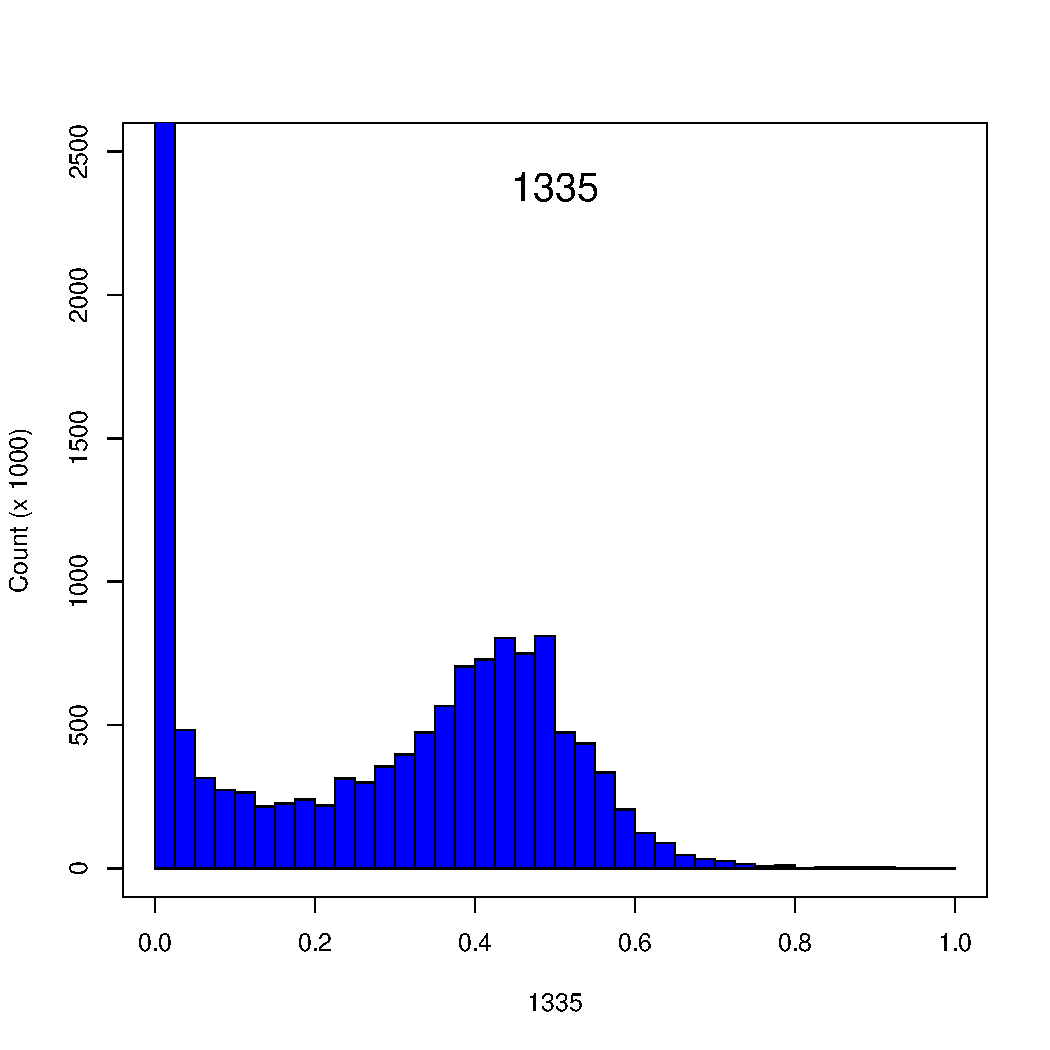
\includegraphics[width=\maxwidth]{Fig1-mscat-figs/unnamed-chunk-20-1} 

\end{knitrout}
\begin{knitrout}\footnotesize
\definecolor{shadecolor}{rgb}{0.969, 0.969, 0.969}\color{fgcolor}\begin{kframe}
\begin{alltt}
\hlcom{# sample scatter-smooth for debugging }
\hlcom{#pdf('scatter15-35-j2T',5,5)}
\hlkwd{smoothScatter}\hlstd{(nrfall[samp,}\hlnum{7}\hlstd{], nrfall[samp,st],} \hlkwc{pch}\hlstd{=}\hlstr{'.'}\hlstd{,} \hlkwc{cex}\hlstd{=}\hlnum{2}\hlstd{,} \hlkwc{col}\hlstd{=}\hlstr{'gray66'}\hlstd{,} \hlkwc{nrpoints}\hlstd{=}\hlnum{200}\hlstd{,}
              \hlkwc{transformation}\hlstd{=}\hlkwd{xformer}\hlstd{(}\hlnum{20}\hlstd{,}\hlnum{.2}\hlstd{,}\hlnum{.03}\hlstd{,}\hlnum{0.33}\hlstd{),}
              \hlkwc{xlab}\hlstd{=}\hlstr{''}\hlstd{,} \hlkwc{xlim}\hlstd{=}\hlnum{0}\hlopt{:}\hlnum{1}\hlstd{,} \hlkwc{xaxp}\hlstd{=}\hlkwd{c}\hlstd{(}\hlnum{0}\hlstd{,}\hlnum{1}\hlstd{,}\hlnum{4}\hlstd{),}
              \hlkwc{ylab}\hlstd{=}\hlstr{''}\hlstd{,} \hlkwc{ylim}\hlstd{=}\hlnum{0}\hlopt{:}\hlnum{1}\hlstd{,} \hlkwc{yaxp}\hlstd{=}\hlkwd{c}\hlstd{(}\hlnum{0}\hlstd{,}\hlnum{1}\hlstd{,}\hlnum{4}\hlstd{))}
\end{alltt}
\end{kframe}
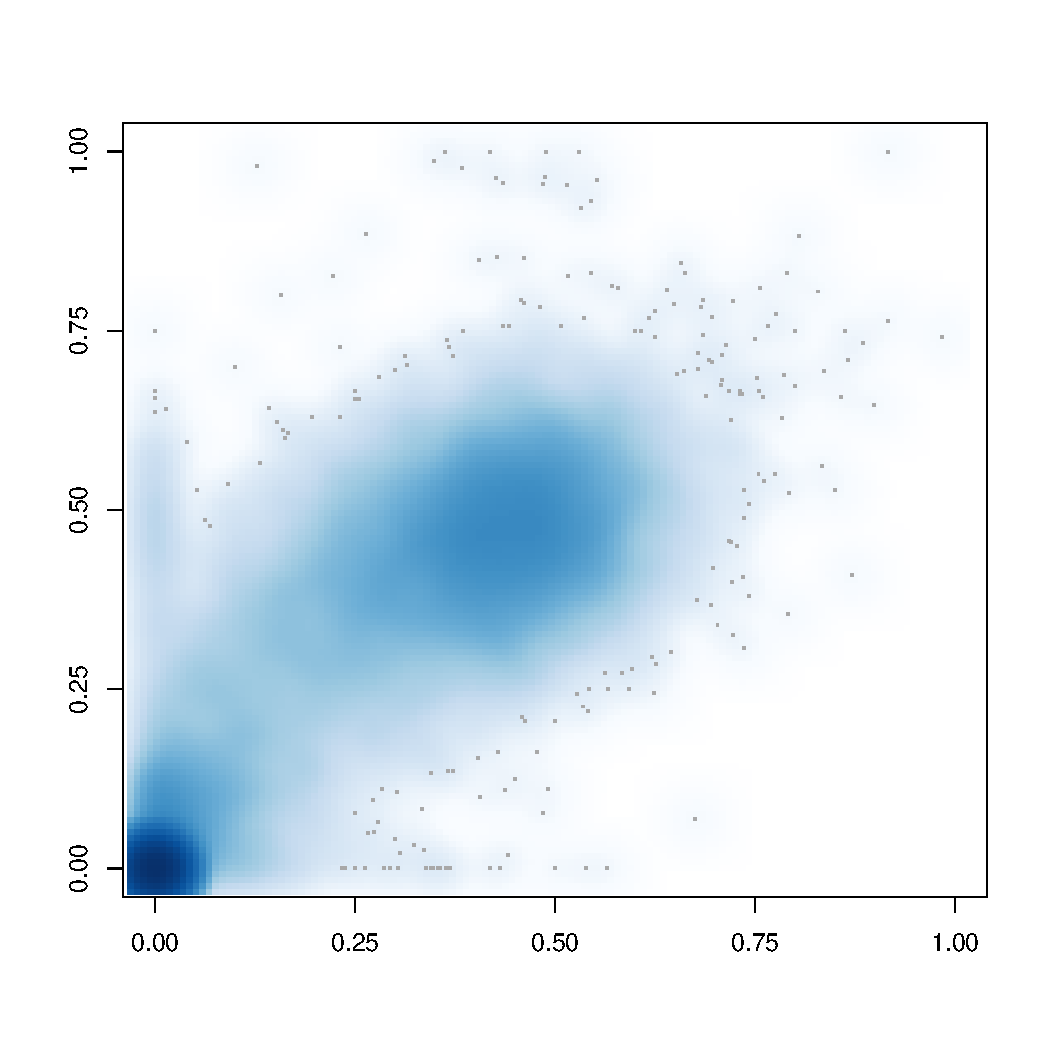
\includegraphics[width=\maxwidth]{Fig1-mscat-figs/unnamed-chunk-21-1} 
\begin{kframe}\begin{alltt}
\hlcom{#dev.off()}
\end{alltt}
\end{kframe}
\end{knitrout}

\begin{knitrout}\footnotesize
\definecolor{shadecolor}{rgb}{0.969, 0.969, 0.969}\color{fgcolor}\begin{kframe}
\begin{alltt}
\hlcom{# Main fig 1 & supp Fig S6: smoothScatter of joint R, with marginal histograms.}
\hlcom{# Mostly circa 10/2015.}
\hlcom{# TO DO, maybe: }
\hlcom{#   5 ticks on x,y (but still 3 labels)?}
\hlcom{#   y-ticks (no lables) on right scatter}
\hlcom{#   y ticks on histos?}
\hlcom{#   some marker for clipped y in histos?}
\hlcom{#   X: (tried this, doesn't help; change filtering so gyre looks better, maybe get 100 k points or so?)}
\hlcom{#   }
\hlstd{margin.scat} \hlkwb{<-} \hlkwa{function}\hlstd{(}\hlkwc{stxl}\hlstd{=}\hlnum{6}\hlstd{,} \hlkwc{stxr}\hlstd{=}\hlnum{2}\hlstd{,} \hlkwc{sty}\hlstd{=}\hlnum{7}\hlstd{,} \hlkwc{label.panels}\hlstd{=}\hlnum{TRUE}\hlstd{)\{}
  \hlcom{# plot main fig with 2 side-by-side smooth-scatters and marginal histograms}
  \hlcom{# if stxl is NULL, omit left scatter/margin}
  \hlstd{opar} \hlkwb{<-} \hlkwd{par}\hlstd{(}\hlkwc{mar}\hlstd{=}\hlkwd{c}\hlstd{(}\hlnum{0.6}\hlstd{,}\hlnum{0.3}\hlstd{,}\hlnum{0.0}\hlstd{,}\hlnum{0.4}\hlstd{),}\hlkwc{oma}\hlstd{=}\hlkwd{c}\hlstd{(}\hlnum{3}\hlstd{,}\hlnum{4}\hlstd{,}\hlnum{0}\hlstd{,}\hlnum{0}\hlstd{),}\hlkwc{tck}\hlstd{=}\hlopt{-}\hlnum{.02}\hlstd{);} \hlkwd{on.exit}\hlstd{(}\hlkwd{par}\hlstd{(opar))}

  \hlcom{# layout in 2 x 4 grid; '0's provide some spacing}
  \hlkwa{if}\hlstd{(}\hlopt{!}\hlkwd{is.null}\hlstd{(stxl))\{}
    \hlstd{layout.mat} \hlkwb{<-} \hlkwd{matrix}\hlstd{(}\hlkwd{c}\hlstd{(}\hlnum{1}\hlstd{,}\hlnum{0}\hlstd{,}\hlnum{2}\hlstd{,}\hlnum{0}\hlstd{,}\hlnum{4}\hlstd{,}\hlnum{0}\hlstd{,}\hlnum{5}\hlstd{,}\hlnum{3}\hlstd{),}\hlkwc{nrow}\hlstd{=}\hlnum{2}\hlstd{,}\hlkwc{byrow}\hlstd{=T)}
  \hlstd{\}} \hlkwa{else} \hlstd{\{}
    \hlstd{layout.mat} \hlkwb{<-} \hlkwd{matrix}\hlstd{(}\hlkwd{c}\hlstd{(}\hlnum{0}\hlstd{,}\hlnum{0}\hlstd{,}\hlnum{1}\hlstd{,}\hlnum{0}\hlstd{,}\hlnum{0}\hlstd{,}\hlnum{0}\hlstd{,}\hlnum{3}\hlstd{,}\hlnum{2}\hlstd{),}\hlkwc{nrow}\hlstd{=}\hlnum{2}\hlstd{,}\hlkwc{byrow}\hlstd{=T)}
  \hlstd{\}}
  \hlkwd{layout}\hlstd{(layout.mat,} \hlkwc{widths}\hlstd{=}\hlkwd{c}\hlstd{(}\hlnum{2}\hlstd{,}\hlnum{0.2}\hlstd{,}\hlnum{2}\hlstd{,}\hlnum{1}\hlstd{),}\hlkwc{heights}\hlstd{=}\hlkwd{c}\hlstd{(}\hlnum{1}\hlstd{,}\hlnum{2}\hlstd{),}
         \hlkwc{respect}\hlstd{=}\hlkwd{matrix}\hlstd{(}\hlkwd{rep}\hlstd{(}\hlnum{1}\hlstd{,}\hlnum{8}\hlstd{),}\hlkwc{nrow}\hlstd{=}\hlnum{2}\hlstd{,}\hlkwc{byrow}\hlstd{=T))}

  \hlcom{# 1: upper left histo}
  \hlkwa{if}\hlstd{(}\hlopt{!}\hlkwd{is.null}\hlstd{(stxl))\{}
    \hlkwd{gamma.hist}\hlstd{(stxl,}\hlkwc{compact}\hlstd{=T,} \hlkwc{show.count.axis}\hlstd{=T,} \hlkwc{panel.label}\hlstd{=}\hlkwd{ifelse}\hlstd{(label.panels,}\hlstr{'A'}\hlstd{,}\hlstr{''}\hlstd{))}
  \hlstd{\}}

  \hlcom{# 2: upper mid histo}
  \hlkwd{gamma.hist}\hlstd{(stxr,}\hlkwc{compact}\hlstd{=T,} \hlkwc{show.count.axis}\hlstd{=}\hlkwd{is.null}\hlstd{(stxl),} \hlkwc{panel.label}\hlstd{=}\hlkwd{ifelse}\hlstd{(label.panels,}\hlstr{'B'}\hlstd{,}\hlstr{''}\hlstd{))}

  \hlcom{# 3: lower right histo}
  \hlkwd{gamma.hist}\hlstd{(sty,}\hlkwc{rotate}\hlstd{=T,}\hlkwc{compact}\hlstd{=T,} \hlkwc{show.count.axis}\hlstd{=T,} \hlkwc{panel.label}\hlstd{=}\hlkwd{ifelse}\hlstd{(label.panels,}\hlstr{'C'}\hlstd{,}\hlstr{''}\hlstd{))}

  \hlcom{# axis labels}
  \hlstd{xl1} \hlkwb{<-} \hlstr{'R'} \hlcom{# paste('R (',colnames(nrfall)[stxl], ')',sep='') }
  \hlstd{xl2} \hlkwb{<-} \hlstr{'R'} \hlcom{# paste('R (',colnames(nrfall)[stxr], ')',sep='') }
  \hlstd{yl}  \hlkwb{<-} \hlstr{'R'} \hlcom{# paste('R (',colnames(nrfall)[sty],  ')',sep='') }

  \hlcom{# 4: lower left scatter}
  \hlkwa{if}\hlstd{(}\hlopt{!}\hlkwd{is.null}\hlstd{(stxl))\{}
    \hlkwd{smoothScatter}\hlstd{(nrfall[samp,stxl], nrfall[samp,sty],}
                  \hlkwc{pch}\hlstd{=}\hlstr{'.'}\hlstd{,} \hlkwc{cex}\hlstd{=}\hlnum{2}\hlstd{,} \hlkwc{col}\hlstd{=}\hlstr{'gray66'}\hlstd{,} \hlkwc{nrpoints}\hlstd{=}\hlnum{200}\hlstd{,}
                  \hlkwc{transformation}\hlstd{=}\hlkwd{xformer}\hlstd{(}\hlnum{20}\hlstd{,}\hlnum{.2}\hlstd{,}\hlnum{.03}\hlstd{,}\hlnum{0.33}\hlstd{),}
                  \hlkwc{xlab}\hlstd{=xl1,} \hlkwc{xlim}\hlstd{=}\hlnum{0}\hlopt{:}\hlnum{1}\hlstd{,} \hlkwc{xaxp}\hlstd{=}\hlkwd{c}\hlstd{(}\hlnum{0}\hlstd{,}\hlnum{1}\hlstd{,}\hlnum{2}\hlstd{),}
                  \hlkwc{ylab}\hlstd{=yl,}  \hlkwc{ylim}\hlstd{=}\hlnum{0}\hlopt{:}\hlnum{1}\hlstd{,} \hlkwc{yaxp}\hlstd{=}\hlkwd{c}\hlstd{(}\hlnum{0}\hlstd{,}\hlnum{1}\hlstd{,}\hlnum{2}\hlstd{),}\hlkwc{xaxt}\hlstd{=}\hlstr{'s'}\hlstd{,}\hlkwc{yaxt}\hlstd{=}\hlstr{'s'}\hlstd{)}
    \hlkwd{mtext}\hlstd{(xl1,}\hlkwc{side}\hlstd{=}\hlnum{1}\hlstd{,} \hlkwc{line}\hlstd{=}\hlnum{2.5}\hlstd{,} \hlkwc{cex}\hlstd{=}\hlnum{.9}\hlstd{)}
    \hlkwd{mtext}\hlstd{(yl,} \hlkwc{side}\hlstd{=}\hlnum{2}\hlstd{,} \hlkwc{line}\hlstd{=}\hlnum{2.5}\hlstd{,} \hlkwc{cex}\hlstd{=}\hlnum{.9}\hlstd{)}
    \hlkwa{if}\hlstd{(label.panels)\{}\hlkwd{text}\hlstd{(}\hlnum{.10}\hlstd{,} \hlnum{.95}\hlstd{,} \hlstr{'D'}\hlstd{,} \hlkwc{cex}\hlstd{=}\hlnum{1.5}\hlstd{)\}}
  \hlstd{\}}

  \hlcom{# 5: lower mid scatter}
  \hlcom{#eplot(0:1,0:1)}
  \hlkwd{smoothScatter}\hlstd{(nrfall[samp,stxr], nrfall[samp,sty],}
                \hlkwc{pch}\hlstd{=}\hlstr{'.'}\hlstd{,} \hlkwc{cex}\hlstd{=}\hlnum{2}\hlstd{,} \hlkwc{col}\hlstd{=}\hlstr{'gray66'}\hlstd{,} \hlkwc{nrpoints}\hlstd{=}\hlnum{200}\hlstd{,}
                \hlkwc{transformation}\hlstd{=}\hlkwd{xformer}\hlstd{(}\hlnum{20}\hlstd{,}\hlnum{.2}\hlstd{,}\hlnum{.03}\hlstd{,}\hlnum{0.33}\hlstd{),}
                \hlkwc{xlab}\hlstd{=xl2,} \hlkwc{xlim}\hlstd{=}\hlnum{0}\hlopt{:}\hlnum{1}\hlstd{,} \hlkwc{xaxp}\hlstd{=}\hlkwd{c}\hlstd{(}\hlnum{0}\hlstd{,}\hlnum{1}\hlstd{,}\hlnum{2}\hlstd{),}
                \hlkwc{ylab}\hlstd{=}\hlstr{''}\hlstd{,}  \hlkwc{ylim}\hlstd{=}\hlnum{0}\hlopt{:}\hlnum{1}\hlstd{,} \hlkwc{yaxp}\hlstd{=}\hlkwd{c}\hlstd{(}\hlnum{0}\hlstd{,}\hlnum{1}\hlstd{,}\hlnum{2}\hlstd{),}\hlkwc{xaxt}\hlstd{=}\hlstr{'s'}\hlstd{,}\hlkwc{yaxt}\hlstd{=}\hlkwd{ifelse}\hlstd{(}\hlkwd{is.null}\hlstd{(stxl),}\hlstr{'s'}\hlstd{,}\hlstr{'n'}\hlstd{))}
  \hlkwd{mtext}\hlstd{(xl2,} \hlkwc{side}\hlstd{=}\hlnum{1}\hlstd{,} \hlkwc{line}\hlstd{=}\hlnum{2.5}\hlstd{,} \hlkwc{cex}\hlstd{=}\hlnum{.9}\hlstd{)}
  \hlkwa{if}\hlstd{(}\hlkwd{is.null}\hlstd{(stxl))\{}
    \hlkwd{mtext}\hlstd{(yl,} \hlkwc{side}\hlstd{=}\hlnum{2}\hlstd{,} \hlkwc{line}\hlstd{=}\hlnum{2.5}\hlstd{,} \hlkwc{cex}\hlstd{=}\hlnum{.9}\hlstd{)}
  \hlstd{\}}
  \hlkwa{if}\hlstd{(label.panels)\{}\hlkwd{text}\hlstd{(}\hlnum{.10}\hlstd{,} \hlnum{.95}\hlstd{,} \hlstr{'E'}\hlstd{,} \hlkwc{cex}\hlstd{=}\hlnum{1.5}\hlstd{)\}}
\hlstd{\}}
\end{alltt}
\end{kframe}
\end{knitrout}

Repeating, the chatter from the call building \texttt{filt99} defines the data being summarized in these plots:

\begin{knitrout}\footnotesize
\definecolor{shadecolor}{rgb}{0.969, 0.969, 0.969}\color{fgcolor}\begin{kframe}
\begin{alltt}
\hlkwd{cat}\hlstd{(filt99}\hlopt{$}\hlstd{chatter)}
\end{alltt}
\begin{verbatim}
# null mask 3042585 positions.
# nrf.6plus1: From a region of length: 3042585 we identified all positions satisfying:
# 10 <= coverage <= 120 in *all* 7 isolates,
# and having 0.1 <= nr.frac <= 1.0 in *at least 1* of them.
# In these positions, counts <= 0 were forced to zero.
# Nonref fraction includes only the max nonref count.
# From these 35291 positions, we sampled 35291 to plot.
\end{verbatim}
\end{kframe}
\end{knitrout}
\begin{knitrout}\footnotesize
\definecolor{shadecolor}{rgb}{0.969, 0.969, 0.969}\color{fgcolor}\begin{kframe}
\begin{alltt}
\hlkwd{pdf}\hlstd{(}\hlkwd{fpath}\hlstd{(}\hlstr{'mscat-6-2-7'}\hlstd{),} \hlkwc{width}\hlstd{=}\hlnum{6.5}\hlstd{,} \hlkwc{height}\hlstd{=}\hlnum{4}\hlstd{)}
\hlkwd{margin.scat}\hlstd{(}\hlnum{6}\hlstd{,}\hlnum{2}\hlstd{,}\hlnum{7}\hlstd{,}\hlkwc{label.panels}\hlstd{=}\hlnum{TRUE}\hlstd{)}
\end{alltt}
\begin{verbatim}
# Counts clipped at 2500 ; Top 5: 16283 2126 1619 1160 813
# Counts clipped at 2500 ; Top 5: 24452 925 865 841 719
# Counts clipped at 2500 ; Top 5: 25041 811 804 749 728
\end{verbatim}
\begin{alltt}
\hlkwd{dev.off}\hlstd{()}
\end{alltt}
\begin{verbatim}
# pdf 
#   2
\end{verbatim}
\end{kframe}
\end{knitrout}
\begin{knitrout}\footnotesize
\definecolor{shadecolor}{rgb}{0.969, 0.969, 0.969}\color{fgcolor}\begin{kframe}
\begin{alltt}
\hlkwd{pdf}\hlstd{(}\hlkwd{fpath}\hlstd{(}\hlstr{'mscat-1-4-7'}\hlstd{),} \hlkwc{width}\hlstd{=}\hlnum{6.5}\hlstd{,} \hlkwc{height}\hlstd{=}\hlnum{4}\hlstd{)}
\hlkwd{margin.scat}\hlstd{(}\hlnum{1}\hlstd{,}\hlnum{4}\hlstd{,}\hlnum{7}\hlstd{)}
\end{alltt}
\begin{verbatim}
# Counts clipped at 2500 ; Top 5: 24172 942 697 689 670
# Counts clipped at 2500 ; Top 5: 20258 4625 950 731 587
# Counts clipped at 2500 ; Top 5: 25041 811 804 749 728
\end{verbatim}
\begin{alltt}
\hlkwd{dev.off}\hlstd{()}
\end{alltt}
\begin{verbatim}
# pdf 
#   2
\end{verbatim}
\end{kframe}
\end{knitrout}
\begin{knitrout}\footnotesize
\definecolor{shadecolor}{rgb}{0.969, 0.969, 0.969}\color{fgcolor}\begin{kframe}
\begin{alltt}
\hlkwd{pdf}\hlstd{(}\hlkwd{fpath}\hlstd{(}\hlstr{'mscat-5-3-7'}\hlstd{),} \hlkwc{width}\hlstd{=}\hlnum{6.5}\hlstd{,} \hlkwc{height}\hlstd{=}\hlnum{4}\hlstd{)}
\hlkwd{margin.scat}\hlstd{(}\hlnum{5}\hlstd{,}\hlnum{3}\hlstd{,}\hlnum{7}\hlstd{)}
\end{alltt}
\begin{verbatim}
# Counts clipped at 2500 ; Top 5: 24248 1043 890 871 730
# Counts clipped at 2500 ; Top 5: 15320 2019 1327 975 931
# Counts clipped at 2500 ; Top 5: 25041 811 804 749 728
\end{verbatim}
\begin{alltt}
\hlkwd{dev.off}\hlstd{()}
\end{alltt}
\begin{verbatim}
# pdf 
#   2
\end{verbatim}
\end{kframe}
\end{knitrout}
\begin{knitrout}\footnotesize
\definecolor{shadecolor}{rgb}{0.969, 0.969, 0.969}\color{fgcolor}\begin{kframe}
\begin{alltt}
\hlkwd{pdf}\hlstd{(}\hlkwd{fpath}\hlstd{(}\hlstr{'mscat-null-3-6'}\hlstd{),} \hlkwc{width}\hlstd{=}\hlnum{6.5}\hlstd{,} \hlkwc{height}\hlstd{=}\hlnum{4}\hlstd{)}
\hlkwd{margin.scat}\hlstd{(}\hlkwa{NULL}\hlstd{,}\hlnum{3}\hlstd{,}\hlnum{6}\hlstd{)} \hlcom{# need 1 x 1 version here, rather than 1 x 2}
\end{alltt}
\begin{verbatim}
# Counts clipped at 2500 ; Top 5: 15320 2019 1327 975 931
# Counts clipped at 2500 ; Top 5: 16283 2126 1619 1160 813
\end{verbatim}
\begin{alltt}
\hlkwd{dev.off}\hlstd{()}
\end{alltt}
\begin{verbatim}
# pdf 
#   2
\end{verbatim}
\end{kframe}
\end{knitrout}

\noindent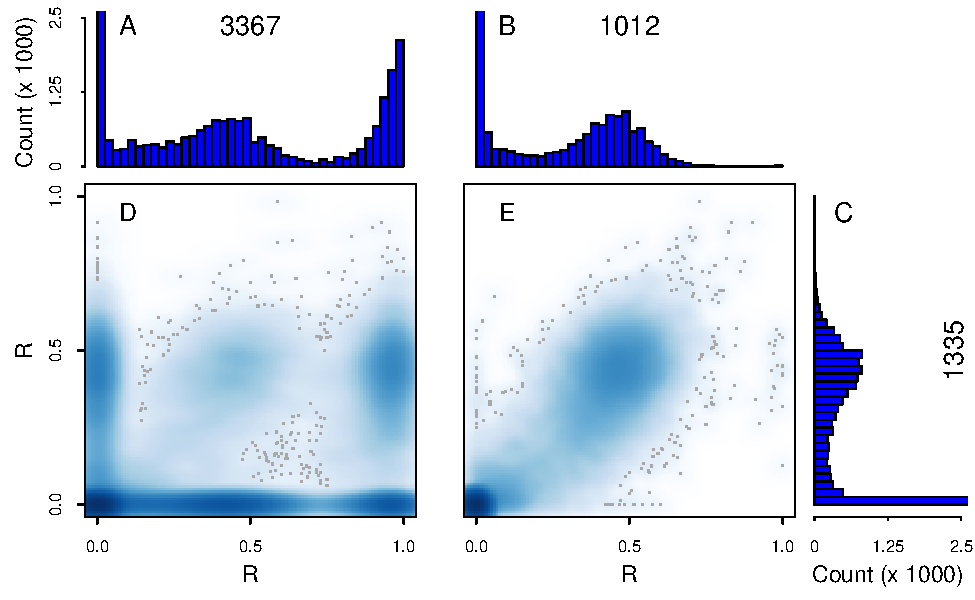
\includegraphics{Fig1-mscat-figs/mscat-6-2-7.pdf}

\noindent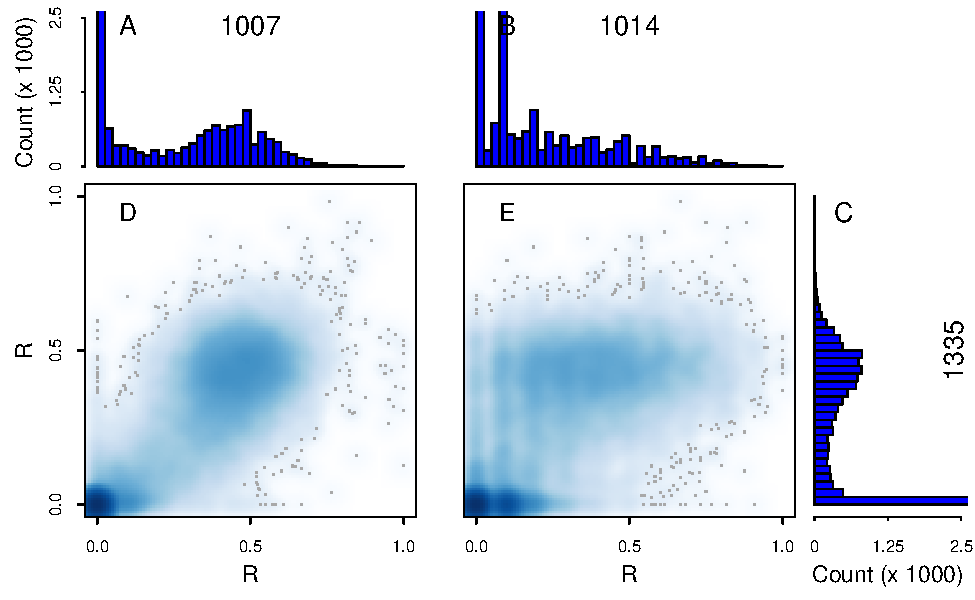
\includegraphics{Fig1-mscat-figs/mscat-1-4-7.pdf}

\noindent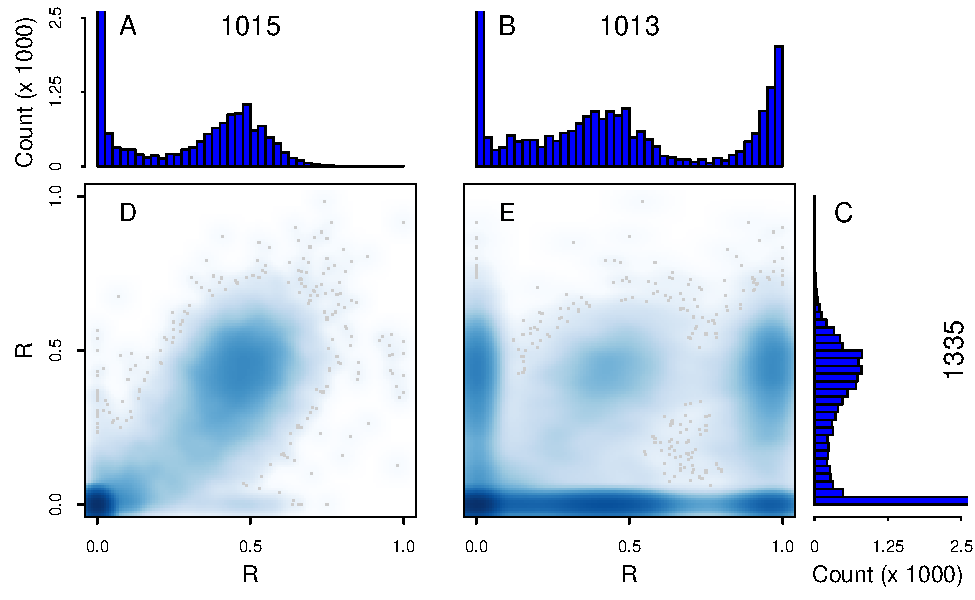
\includegraphics{Fig1-mscat-figs/mscat-5-3-7.pdf}

\noindent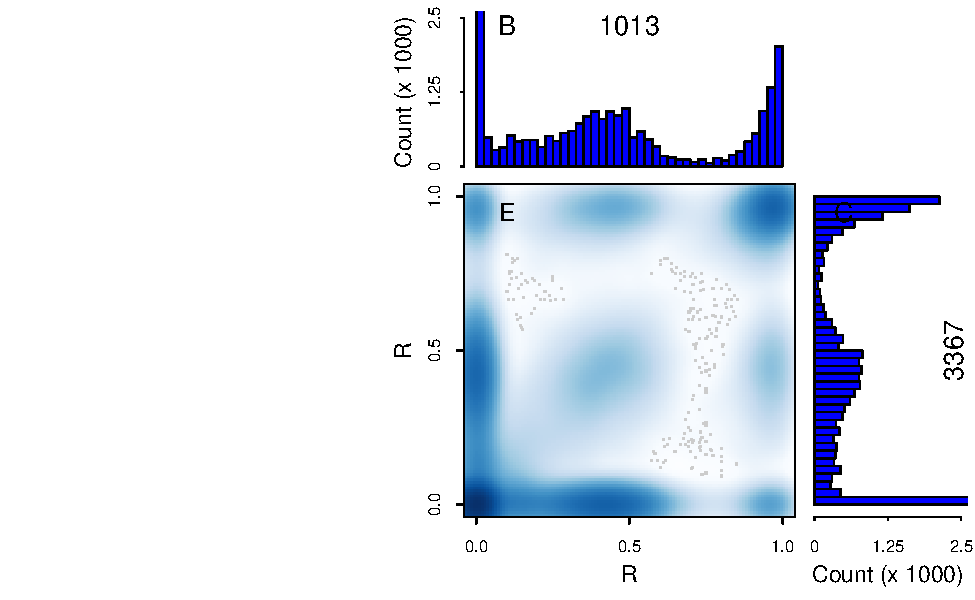
\includegraphics{Fig1-mscat-figs/mscat-null-3-6.pdf}

\section{``6+1'' with dots}

Generate versions of the ``6+1'' plots (dots, not smoothed), with various filtering parameters.  This was an earlier idea for displaying the data.  I like the smooth-scatters better; keeping this ``just in case.''

\begin{knitrout}\footnotesize
\definecolor{shadecolor}{rgb}{0.969, 0.969, 0.969}\color{fgcolor}\begin{kframe}
\begin{alltt}
\hlkwd{pack.debug}\hlstd{()}
\hlstd{yaxislabels} \hlkwb{<-} \hlstr{''} \hlcom{### some bug in compactr; this var sometimes used but undefined}
\hlstd{make.dots} \hlkwb{<-} \hlnum{TRUE}
\hlkwa{if}\hlstd{(make.dots)\{}
  \hlkwd{pdf}\hlstd{(}\hlkwd{fpath}\hlstd{(}\hlstr{'6+1julie0F'}\hlstd{),} \hlkwc{width}\hlstd{=}\hlnum{1.75}\hlstd{,} \hlkwc{height}\hlstd{=}\hlnum{8.25}\hlstd{)}
  \hlkwd{set.seed}\hlstd{(}\hlnum{1}\hlstd{)}
  \hlstd{filt1} \hlkwb{<-} \hlkwd{nrf.6plus1}\hlstd{(}\hlkwc{snp.tables}\hlstd{=snp.tables,}\hlkwc{sample}\hlstd{=}\hlnum{10000}\hlstd{,}\hlkwc{pch}\hlstd{=}\hlstr{'.'}\hlstd{,}\hlkwc{export}\hlstd{=T,}\hlkwc{julie.filter1}\hlstd{=}\hlnum{0}\hlstd{,}\hlkwc{julie.filter2}\hlstd{=F)}
  \hlkwd{dev.off}\hlstd{()}
\hlstd{\}}
\end{alltt}
\begin{verbatim}
# null mask 3042585 positions.
# nrf.6plus1: From a region of length: 3042585 we identified all positions satisfying: 
#  21 <= coverage <= 150 in *all* 7 isolates, 
# and having 0.1 <= nr.frac <= 1.0 in *at least 1* of them. 
# From these 5213 positions, we sampled 10000 to plot.
# pdf 
#   2
\end{verbatim}
\end{kframe}
\end{knitrout}
\begin{knitrout}\footnotesize
\definecolor{shadecolor}{rgb}{0.969, 0.969, 0.969}\color{fgcolor}\begin{kframe}
\begin{alltt}
\hlkwa{if}\hlstd{(make.dots)\{}
  \hlkwd{pdf}\hlstd{(}\hlkwd{fpath}\hlstd{(}\hlstr{'6+1julie1F'}\hlstd{),} \hlkwc{width}\hlstd{=}\hlnum{1.75}\hlstd{,} \hlkwc{height}\hlstd{=}\hlnum{8.25}\hlstd{)}
  \hlkwd{set.seed}\hlstd{(}\hlnum{1}\hlstd{)}
  \hlstd{filt2} \hlkwb{<-} \hlkwd{nrf.6plus1}\hlstd{(}\hlkwc{snp.tables}\hlstd{=snp.tables,}\hlkwc{sample}\hlstd{=}\hlnum{10000}\hlstd{,}\hlkwc{pch}\hlstd{=}\hlstr{'.'}\hlstd{,}\hlkwc{export}\hlstd{=T,}\hlkwc{julie.filter1}\hlstd{=}\hlnum{1}\hlstd{,}\hlkwc{julie.filter2}\hlstd{=F)}
  \hlkwd{dev.off}\hlstd{()}
\hlstd{\}}
\end{alltt}
\begin{verbatim}
# null mask 3042585 positions.
# nrf.6plus1: From a region of length: 3042585 we identified all positions satisfying: 
#  21 <= coverage <= 150 in *all* 7 isolates, 
# and having 0.1 <= nr.frac <= 1.0 in *at least 1* of them. 
# From these 5213 positions, we sampled 10000 to plot.
# pdf 
#   2
\end{verbatim}
\end{kframe}
\end{knitrout}
\begin{knitrout}\footnotesize
\definecolor{shadecolor}{rgb}{0.969, 0.969, 0.969}\color{fgcolor}\begin{kframe}
\begin{alltt}
\hlkwa{if}\hlstd{(make.dots)\{}
  \hlkwd{pdf}\hlstd{(}\hlkwd{fpath}\hlstd{(}\hlstr{'6+1julie2F'}\hlstd{),} \hlkwc{width}\hlstd{=}\hlnum{1.75}\hlstd{,} \hlkwc{height}\hlstd{=}\hlnum{8.25}\hlstd{)}
  \hlkwd{set.seed}\hlstd{(}\hlnum{1}\hlstd{)}
  \hlstd{filt3} \hlkwb{<-} \hlkwd{nrf.6plus1}\hlstd{(}\hlkwc{snp.tables}\hlstd{=snp.tables,}\hlkwc{sample}\hlstd{=}\hlnum{10000}\hlstd{,}\hlkwc{pch}\hlstd{=}\hlstr{'.'}\hlstd{,}\hlkwc{export}\hlstd{=T,}\hlkwc{julie.filter1}\hlstd{=}\hlnum{2}\hlstd{,}\hlkwc{julie.filter2}\hlstd{=F)}
  \hlkwd{dev.off}\hlstd{()}
\hlstd{\}}
\end{alltt}
\begin{verbatim}
# null mask 3042585 positions.
# nrf.6plus1: From a region of length: 3042585 we identified all positions satisfying: 
#  21 <= coverage <= 150 in *all* 7 isolates, 
# and having 0.1 <= nr.frac <= 1.0 in *at least 1* of them. 
# From these 5213 positions, we sampled 10000 to plot.
# pdf 
#   2
\end{verbatim}
\end{kframe}
\end{knitrout}
\begin{knitrout}\footnotesize
\definecolor{shadecolor}{rgb}{0.969, 0.969, 0.969}\color{fgcolor}\begin{kframe}
\begin{alltt}
\hlkwa{if}\hlstd{(make.dots)\{}
  \hlkwd{pdf}\hlstd{(}\hlkwd{fpath}\hlstd{(}\hlstr{'6+1julie0T'}\hlstd{),} \hlkwc{width}\hlstd{=}\hlnum{1.75}\hlstd{,} \hlkwc{height}\hlstd{=}\hlnum{8.25}\hlstd{)}
  \hlkwd{set.seed}\hlstd{(}\hlnum{1}\hlstd{)}
  \hlstd{filt4} \hlkwb{<-} \hlkwd{nrf.6plus1}\hlstd{(}\hlkwc{snp.tables}\hlstd{=snp.tables,}\hlkwc{sample}\hlstd{=}\hlnum{10000}\hlstd{,}\hlkwc{pch}\hlstd{=}\hlstr{'.'}\hlstd{,}\hlkwc{export}\hlstd{=T,}\hlkwc{julie.filter1}\hlstd{=}\hlnum{0}\hlstd{,}\hlkwc{julie.filter2}\hlstd{=T)}
  \hlkwd{dev.off}\hlstd{()}
\hlstd{\}}
\end{alltt}
\begin{verbatim}
# null mask 3042585 positions.
# nrf.6plus1: From a region of length: 3042585 we identified all positions satisfying: 
#  21 <= coverage <= 150 in *all* 7 isolates, 
# and having 0.1 <= nr.frac <= 1.0 in *at least 1* of them. 
# From these 5213 positions, we sampled 10000 to plot.
# pdf 
#   2
\end{verbatim}
\end{kframe}
\end{knitrout}
\begin{knitrout}\footnotesize
\definecolor{shadecolor}{rgb}{0.969, 0.969, 0.969}\color{fgcolor}\begin{kframe}
\begin{alltt}
\hlkwa{if}\hlstd{(make.dots)\{}
  \hlkwd{pdf}\hlstd{(}\hlkwd{fpath}\hlstd{(}\hlstr{'6+1julie1T'}\hlstd{),} \hlkwc{width}\hlstd{=}\hlnum{1.75}\hlstd{,} \hlkwc{height}\hlstd{=}\hlnum{8.25}\hlstd{)}
  \hlkwd{set.seed}\hlstd{(}\hlnum{1}\hlstd{)}
  \hlstd{filt5} \hlkwb{<-} \hlkwd{nrf.6plus1}\hlstd{(}\hlkwc{snp.tables}\hlstd{=snp.tables,}\hlkwc{sample}\hlstd{=}\hlnum{10000}\hlstd{,}\hlkwc{pch}\hlstd{=}\hlstr{'.'}\hlstd{,}\hlkwc{export}\hlstd{=T,}\hlkwc{julie.filter1}\hlstd{=}\hlnum{1}\hlstd{,}\hlkwc{julie.filter2}\hlstd{=T)}
  \hlkwd{dev.off}\hlstd{()}
\hlstd{\}}
\end{alltt}
\begin{verbatim}
# null mask 3042585 positions.
# nrf.6plus1: From a region of length: 3042585 we identified all positions satisfying: 
#  21 <= coverage <= 150 in *all* 7 isolates, 
# and having 0.1 <= nr.frac <= 1.0 in *at least 1* of them. 
# From these 5213 positions, we sampled 10000 to plot.
# pdf 
#   2
\end{verbatim}
\end{kframe}
\end{knitrout}
\begin{knitrout}\footnotesize
\definecolor{shadecolor}{rgb}{0.969, 0.969, 0.969}\color{fgcolor}\begin{kframe}
\begin{alltt}
\hlkwa{if}\hlstd{(make.dots)\{}
  \hlkwd{pdf}\hlstd{(}\hlkwd{fpath}\hlstd{(}\hlstr{'6+1julie2T'}\hlstd{),} \hlkwc{width}\hlstd{=}\hlnum{1.75}\hlstd{,} \hlkwc{height}\hlstd{=}\hlnum{8.25}\hlstd{)}
  \hlkwd{set.seed}\hlstd{(}\hlnum{1}\hlstd{)}
  \hlstd{filt6} \hlkwb{<-} \hlkwd{nrf.6plus1}\hlstd{(}\hlkwc{snp.tables}\hlstd{=snp.tables,}\hlkwc{sample}\hlstd{=}\hlnum{10000}\hlstd{,}\hlkwc{pch}\hlstd{=}\hlstr{'.'}\hlstd{,}\hlkwc{export}\hlstd{=T,}\hlkwc{julie.filter1}\hlstd{=}\hlnum{2}\hlstd{,}\hlkwc{julie.filter2}\hlstd{=T)}
  \hlkwd{dev.off}\hlstd{()}
\hlstd{\}}
\end{alltt}
\begin{verbatim}
# null mask 3042585 positions.
# nrf.6plus1: From a region of length: 3042585 we identified all positions satisfying: 
#  21 <= coverage <= 150 in *all* 7 isolates, 
# and having 0.1 <= nr.frac <= 1.0 in *at least 1* of them. 
# From these 5213 positions, we sampled 10000 to plot.
# pdf 
#   2
\end{verbatim}
\end{kframe}
\end{knitrout}
\begin{knitrout}\footnotesize
\definecolor{shadecolor}{rgb}{0.969, 0.969, 0.969}\color{fgcolor}\begin{kframe}
\begin{alltt}
\hlkwa{if}\hlstd{(make.dots)\{}
  \hlcom{# verify consistent sampling}
  \hlkwd{all}\hlstd{(filt1}\hlopt{$}\hlstd{sample}\hlopt{==}\hlstd{filt2}\hlopt{$}\hlstd{sample)} \hlopt{&&}
  \hlkwd{all}\hlstd{(filt1}\hlopt{$}\hlstd{sample}\hlopt{==}\hlstd{filt3}\hlopt{$}\hlstd{sample)} \hlopt{&&}
  \hlkwd{all}\hlstd{(filt1}\hlopt{$}\hlstd{sample}\hlopt{==}\hlstd{filt4}\hlopt{$}\hlstd{sample)} \hlopt{&&}
  \hlkwd{all}\hlstd{(filt1}\hlopt{$}\hlstd{sample}\hlopt{==}\hlstd{filt5}\hlopt{$}\hlstd{sample)} \hlopt{&&}
  \hlkwd{all}\hlstd{(filt1}\hlopt{$}\hlstd{sample}\hlopt{==}\hlstd{filt6}\hlopt{$}\hlstd{sample)}
\hlstd{\}}
\end{alltt}
\begin{verbatim}
# [1] TRUE
\end{verbatim}
\end{kframe}
\end{knitrout}

\noindent%
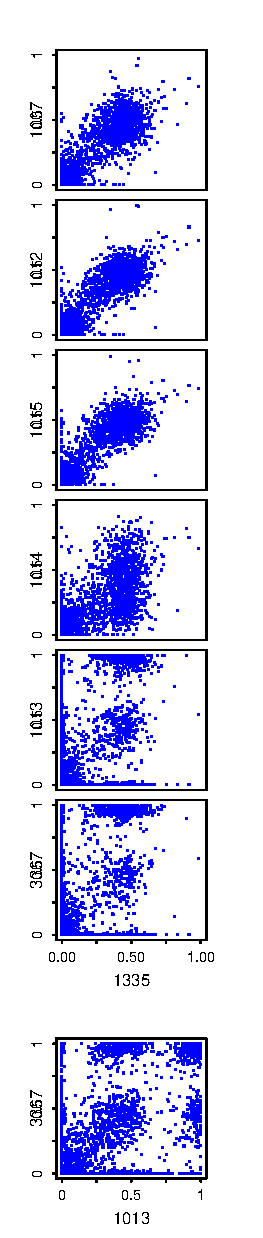
\includegraphics{Fig1-mscat-figs/6+1julie0F.pdf}%
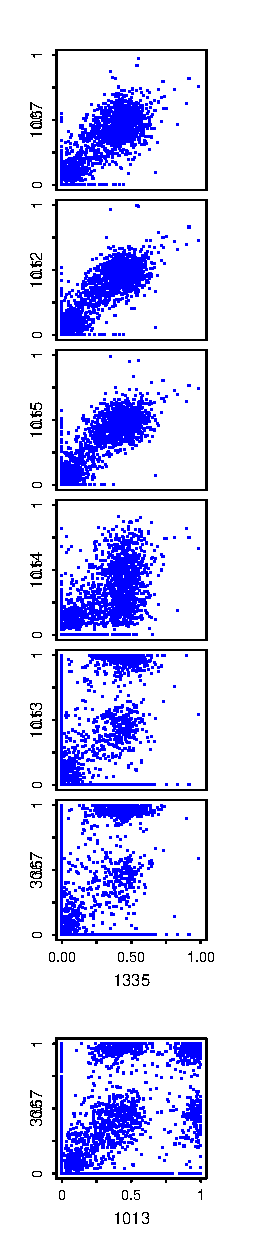
\includegraphics{Fig1-mscat-figs/6+1julie1F.pdf}%
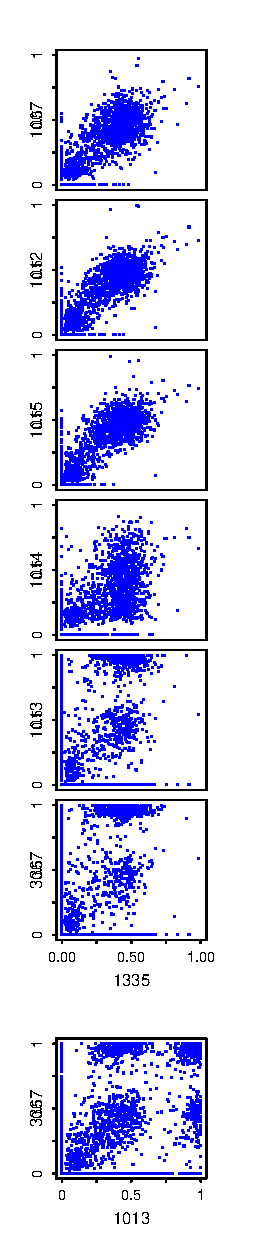
\includegraphics{Fig1-mscat-figs/6+1julie2F.pdf}

\noindent%
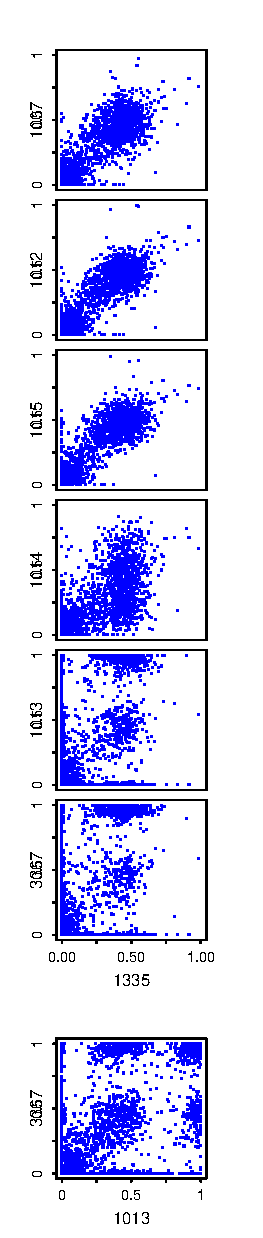
\includegraphics{Fig1-mscat-figs/6+1julie0T.pdf}%
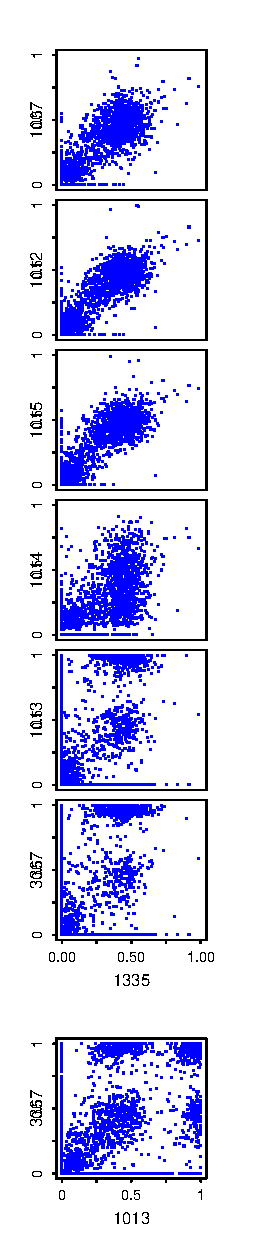
\includegraphics{Fig1-mscat-figs/6+1julie1T.pdf}%
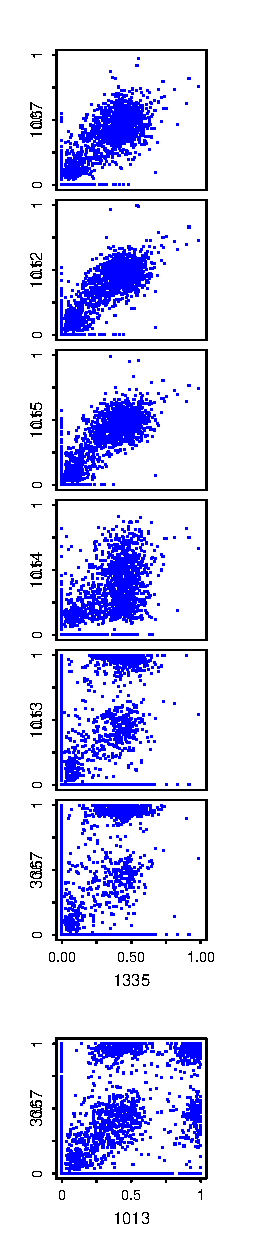
\includegraphics{Fig1-mscat-figs/6+1julie2T.pdf}

Proposed caption: ...

\section{Post-Analysis}\label{sec:post}
The figure plots total nonref count over coverage, without regard to how nonref count is split among the three possibilities or to whether the same nonref nucleotide is dominant in different strains.  Julie expressed concerned about this; should we change it? It is at least confusing, so we need to think how to explain it. (Following analysis mostly based on the un-Julie-filtered data for the 1st plot.)

\subsection{Extract shared positions used in pairwise plots}

Plot function returns data useful for making the plots themselves, but we need to cross-reference this to the original SNP tables.

\begin{knitrout}\scriptsize
\definecolor{shadecolor}{rgb}{0.969, 0.969, 0.969}\color{fgcolor}\begin{kframe}
\begin{alltt}
\hlkwd{str}\hlstd{(filt1)}
\end{alltt}
\begin{verbatim}
# List of 2
#  $ sample: int [1:5213] 1 2 3 4 5 6 7 8 9 10 ...
#  $ nrfall: num [1:5213, 1:7] 0.0741 0 0 0.0385 0 ...
#   ..- attr(*, "dimnames")=List of 2
#   .. ..$ : chr [1:5213] "Chr1:118" "Chr1:128" "Chr1:279" "Chr1:567" ...
#   .. ..$ : chr [1:7] "1007" "1012" "1013" "1014" ...
\end{verbatim}
\end{kframe}
\end{knitrout}

Re-form indices into snp.tables from \texttt{nrfall} row names, and, as a sanity check, visually spot check that these satisfy the expected filters.

\begin{knitrout}\scriptsize
\definecolor{shadecolor}{rgb}{0.969, 0.969, 0.969}\color{fgcolor}\begin{kframe}
\begin{alltt}
\hlstd{selected} \hlkwb{<-} \hlkwd{as.integer}\hlstd{(}\hlkwd{sub}\hlstd{(}\hlstr{'Chr1:'}\hlstd{,} \hlstr{''}\hlstd{,} \hlkwd{rownames}\hlstd{(filt1}\hlopt{$}\hlstd{nrfall),} \hlkwc{fixed}\hlstd{=T))}
\hlkwd{seecounts}\hlstd{(selected[}\hlnum{1}\hlopt{:}\hlnum{5}\hlstd{],}\hlkwc{snp.tables}\hlstd{=snp.tables)}
\end{alltt}
\begin{verbatim}
#     chr  pos Ref Strain   A   G   C   T SNP  exon indel nrf rat
# 1  Chr1  118   A                                               
# 2                  1007  50   4   0   0   0 FALSE FALSE        
# 3                  1012  88   5   0   0   0 FALSE FALSE        
# 4                  1013 105   4   0   0   0 FALSE FALSE        
# 5                  1014  29   4   0   0   0 FALSE FALSE        
# 6                  1015  72   3   0   0   0 FALSE FALSE        
# 7                  3367  67   5   0   0   0 FALSE FALSE        
# 8                  1335 139   7   0   0   0 FALSE FALSE        
# 9  Chr1  128   C                                               
# 10                 1007   0   0  46   0   0 FALSE FALSE        
# 11                 1012   0   0  64   0   0 FALSE FALSE        
# 12                 1013   0   0  53  15   0 FALSE FALSE        
# 13                 1014   0   0  25   0   0 FALSE FALSE        
# 14                 1015   0   0  59   0   0 FALSE FALSE        
# 15                 3367   0   0  25   6   0 FALSE FALSE        
# 16                 1335   0   0 136   1   0 FALSE FALSE        
# 17 Chr1  279   T                                               
# 18                 1007   0   0   0  46   0 FALSE FALSE        
# 19                 1012   0   0   0  73   0 FALSE FALSE        
# 20                 1013  36   0   0  74   0 FALSE FALSE        
# 21                 1014   0   1   0  40   0 FALSE FALSE        
# 22                 1015   0   0   0  89   0 FALSE FALSE        
# 23                 3367  20   0   0  37   0 FALSE FALSE        
# 24                 1335   0   0   0 139   0 FALSE FALSE        
# 25 Chr1  567   T                                               
# 26                 1007   0   0   1  25   0  TRUE FALSE        
# 27                 1012   0   0  14  39   1  TRUE FALSE        
# 28                 1013   0   0  13  87   0  TRUE FALSE        
# 29                 1014   0   1   0  23   0  TRUE FALSE        
# 30                 1015   0   0   8  40   1  TRUE FALSE        
# 31                 3367   0   0  16  38   1  TRUE FALSE        
# 32                 1335   0   0   2  99   0  TRUE FALSE        
# 33 Chr1 1878   G                                               
# 34                 1007   0  26   0   0   0  TRUE FALSE        
# 35                 1012   0  46   0   0   0  TRUE FALSE        
# 36                 1013   9  47   0   0   0  TRUE FALSE        
# 37                 1014   0  24   0   0   0  TRUE FALSE        
# 38                 1015   0  57   0   0   0  TRUE FALSE        
# 39                 3367   0  22   0   0   0  TRUE FALSE        
# 40                 1335   0 135   0   0   0  TRUE FALSE
\end{verbatim}
\begin{alltt}
\hlstd{n.selected} \hlkwb{<-} \hlkwd{length}\hlstd{(selected)}
\hlkwa{if}\hlstd{(}\hlopt{!}\hlkwd{exists}\hlstd{(}\hlstr{'n.selected'}\hlstd{))\{n.selected} \hlkwb{<-} \hlnum{NA}\hlstd{\}} \hlcom{### bug chasing...}
\end{alltt}
\end{kframe}
\end{knitrout}

Recast the selection as a long Bool vector, instead of a short vector of indices, for convenience in masking \texttt{snp.tables}.

\begin{knitrout}\scriptsize
\definecolor{shadecolor}{rgb}{0.969, 0.969, 0.969}\color{fgcolor}\begin{kframe}
\begin{alltt}
\hlstd{longsel} \hlkwb{<-} \hlkwd{vector}\hlstd{(}\hlstr{'logical'}\hlstd{,}\hlkwd{nrow}\hlstd{(snp.tables[[}\hlnum{1}\hlstd{]]))}
\hlstd{longsel[selected]} \hlkwb{<-} \hlstd{T}
\end{alltt}
\end{kframe}
\end{knitrout}

Build a set of subtables with just selected positions.

\begin{knitrout}\footnotesize
\definecolor{shadecolor}{rgb}{0.969, 0.969, 0.969}\color{fgcolor}\begin{kframe}
\begin{alltt}
\hlstd{seltab} \hlkwb{<-}\hlkwa{NULL}
\hlkwa{for}\hlstd{(st} \hlkwa{in} \hlnum{1}\hlopt{:}\hlnum{7}\hlstd{)\{}
  \hlstd{seltab[[st]]} \hlkwb{<-} \hlstd{snp.tables[[st]][longsel,]}
\hlstd{\}}
\hlkwd{names}\hlstd{(seltab)} \hlkwb{<-} \hlkwd{names}\hlstd{(snp.tables)}
\end{alltt}
\end{kframe}
\end{knitrout}

\subsection{Discordant ``Nonreference Alleles''}
\label{sec:discord}

We need to asses the degree of discordance between selected positions in different strains.  E.g., in particular, how often do we see significant read counts at \emph{different} nonreference nucleotides at selected positions?

The following text and code snippet is taken verbatim from \texttt{shared-snps.rnw}, svn 557, except that I have added \texttt{snp.tables} as an explicit parameter to the function, and did a common subexpression optimization (which doesn't seem much faster, oh well).

\begin{quote}
For a given strain, the following function returns a vector of 0:4 to indicate which nonreference nucleotide has the
maximum read count at the corresponding position.  The values 1..4 indicate that the max count occurred at A, G, C, T,
resp.  (Ties are resolved arbitrarily ($a<g<c<t$), which possibly deserves further attention.)  The value 0 means all
nonreference counts are below threshold, based \emph{either} on absolute count \emph{or} as a fraction of coverage.
Default only excludes 0 counts.

\begin{knitrout}\footnotesize
\definecolor{shadecolor}{rgb}{0.969, 0.969, 0.969}\color{fgcolor}\begin{kframe}
\begin{alltt}
\hlstd{nref.nuc.new} \hlkwb{<-} \hlkwa{function}\hlstd{(}\hlkwc{strain}\hlstd{=}\hlnum{1}\hlstd{,} \hlkwc{mask}\hlstd{=T,} \hlkwc{thresh.count}\hlstd{=}\hlnum{0}\hlstd{,} \hlkwc{thresh.rate}\hlstd{=}\hlnum{0.0}\hlstd{,}
                         \hlkwc{snp.tables}\hlstd{=snp.tables.01.26.14)\{}
  \hlcom{# extract strain/mask subtable}
  \hlstd{subtab} \hlkwb{<-} \hlstd{snp.tables[[strain]][mask,]}
  \hlcom{# get read count for max nonref nuc}
        \hlstd{nref} \hlkwb{<-} \hlkwd{apply}\hlstd{(subtab[,} \hlkwd{c}\hlstd{(}\hlstr{'a'}\hlstd{,} \hlstr{'g'}\hlstd{,} \hlstr{'c'}\hlstd{,} \hlstr{'t'}\hlstd{)],} \hlnum{1}\hlstd{, max)}
        \hlcom{# where does nref count match a (g,c,t, resp) count}
        \hlstd{as} \hlkwb{<-} \hlkwd{ifelse}\hlstd{(nref} \hlopt{==} \hlstd{subtab[,}\hlstr{'a'}\hlstd{],}\hlnum{1}\hlstd{,}\hlnum{0}\hlstd{)}
        \hlstd{gs} \hlkwb{<-} \hlkwd{ifelse}\hlstd{(nref} \hlopt{==} \hlstd{subtab[,}\hlstr{'g'}\hlstd{],}\hlnum{2}\hlstd{,}\hlnum{0}\hlstd{)}
        \hlstd{cs} \hlkwb{<-} \hlkwd{ifelse}\hlstd{(nref} \hlopt{==} \hlstd{subtab[,}\hlstr{'c'}\hlstd{],}\hlnum{3}\hlstd{,}\hlnum{0}\hlstd{)}
        \hlstd{ts} \hlkwb{<-} \hlkwd{ifelse}\hlstd{(nref} \hlopt{==} \hlstd{subtab[,}\hlstr{'t'}\hlstd{],}\hlnum{4}\hlstd{,}\hlnum{0}\hlstd{)}
        \hlcom{# most positions will show 3 zeros and one of 1:4, so max identifies max nonref count;}
        \hlcom{# ties broken arbitrarily  (a<g<c<t)}
        \hlstd{merge} \hlkwb{<-} \hlkwd{pmax}\hlstd{(as,gs,cs,ts)}
        \hlcom{# but if max nonref count is zero or below threshold, return 0}
        \hlstd{merge[nref} \hlopt{==} \hlnum{0} \hlopt{|} \hlstd{nref} \hlopt{<} \hlstd{thresh.count]} \hlkwb{<-} \hlnum{0}
        \hlstd{merge[nref}\hlopt{/}\hlstd{subtab[,}\hlstr{'Cov'}\hlstd{]} \hlopt{<} \hlstd{thresh.rate]} \hlkwb{<-} \hlnum{0}
        \hlkwd{return}\hlstd{(merge)}
\hlstd{\}}
\end{alltt}
\end{kframe}
\end{knitrout}

\end{quote}

We use this to assess the degree of discordance between strains at the selected positions used for the pairwise scatter plots, with various levels of stringency in the \texttt{thresh.count, thresh.rate} parameters.  [Note: thresh.rate and thresh.count tests are ``strictly less,'' so, e.g., thresh.count=1 does \emph{not} eliminate singleton reads; threshcount=1.1 does.]

\begin{knitrout}\footnotesize
\definecolor{shadecolor}{rgb}{0.969, 0.969, 0.969}\color{fgcolor}\begin{kframe}
\begin{alltt}
\hlstd{nrf.nuc.list} \hlkwb{<-} \hlkwa{function}\hlstd{(}\hlkwc{mask}\hlstd{=longsel,} \hlkwc{thresh.count}\hlstd{=}\hlnum{0}\hlstd{,} \hlkwc{thresh.rate}\hlstd{=}\hlnum{0.0}\hlstd{,} \hlkwc{snp.tables}\hlstd{=snp.tables.01.26.14)\{}
  \hlstd{nrf.nucs} \hlkwb{<-} \hlkwa{NULL}
  \hlkwa{for}\hlstd{(st} \hlkwa{in} \hlnum{1}\hlopt{:}\hlnum{7}\hlstd{)\{}
    \hlstd{nrf.nucs[[st]]} \hlkwb{<-} \hlkwd{nref.nuc.new}\hlstd{(}\hlkwc{strain}\hlstd{=st,} \hlkwc{mask}\hlstd{=mask,} \hlkwc{thresh.count}\hlstd{=thresh.count,}
                                   \hlkwc{thresh.rate}\hlstd{=thresh.rate,} \hlkwc{snp.tables}\hlstd{=snp.tables)}
  \hlstd{\}}
  \hlkwd{return}\hlstd{(nrf.nucs)}
\hlstd{\}}
\hlstd{nrf.nucs1} \hlkwb{<-} \hlkwd{nrf.nuc.list}\hlstd{(}\hlkwc{mask}\hlstd{=T,} \hlkwc{thresh.count}\hlstd{=}\hlnum{0.0}\hlstd{,} \hlkwc{thresh.rate}\hlstd{=}\hlnum{0.00}\hlstd{,} \hlkwc{snp.tables}\hlstd{=seltab)}
\hlstd{nrf.nucs2} \hlkwb{<-} \hlkwd{nrf.nuc.list}\hlstd{(}\hlkwc{mask}\hlstd{=T,} \hlkwc{thresh.count}\hlstd{=}\hlnum{1.1}\hlstd{,} \hlkwc{thresh.rate}\hlstd{=}\hlnum{0.00}\hlstd{,} \hlkwc{snp.tables}\hlstd{=seltab)}
\hlstd{nrf.nucs3} \hlkwb{<-} \hlkwd{nrf.nuc.list}\hlstd{(}\hlkwc{mask}\hlstd{=T,} \hlkwc{thresh.count}\hlstd{=}\hlnum{2.1}\hlstd{,} \hlkwc{thresh.rate}\hlstd{=}\hlnum{0.00}\hlstd{,} \hlkwc{snp.tables}\hlstd{=seltab)}
\hlstd{nrf.nucs4} \hlkwb{<-} \hlkwd{nrf.nuc.list}\hlstd{(}\hlkwc{mask}\hlstd{=T,} \hlkwc{thresh.count}\hlstd{=}\hlnum{0.0}\hlstd{,} \hlkwc{thresh.rate}\hlstd{=}\hlnum{0.05}\hlstd{,} \hlkwc{snp.tables}\hlstd{=seltab)}
\hlcom{# 5 is identical to 4, since singletons are < 0.05, given min.cov=21}
\hlcom{# nrf.nucs5 <- nrf.nuc.list(mask=T, thresh.count=1.1, thresh.rate=0.05, snp.tables=seltab)}
\hlstd{nrf.nucs6} \hlkwb{<-} \hlkwd{nrf.nuc.list}\hlstd{(}\hlkwc{mask}\hlstd{=T,} \hlkwc{thresh.count}\hlstd{=}\hlnum{2.1}\hlstd{,} \hlkwc{thresh.rate}\hlstd{=}\hlnum{0.05}\hlstd{,} \hlkwc{snp.tables}\hlstd{=seltab)}

\hlstd{discordance} \hlkwb{<-} \hlkwa{function}\hlstd{(}\hlkwc{nrf.nucs}\hlstd{,} \hlkwc{snp.tables}\hlstd{=snp.tables.01.26.14)\{}
  \hlcom{# nrf.nucs in 1:4 indicates max nonref nuc is AGCT, resp; 0 means max is 0}
  \hlcom{# 'discord' simply counts positions where these differ between strain i & j}
  \hlstd{discord} \hlkwb{<-} \hlkwd{matrix}\hlstd{(}\hlnum{NA}\hlstd{,}\hlkwc{nrow}\hlstd{=}\hlnum{7}\hlstd{,}\hlkwc{ncol}\hlstd{=}\hlnum{7}\hlstd{)}
  \hlkwd{rownames}\hlstd{(discord)} \hlkwb{<-} \hlkwd{names}\hlstd{(snp.tables)}
  \hlkwd{colnames}\hlstd{(discord)} \hlkwb{<-} \hlkwd{names}\hlstd{(snp.tables)}
  \hlkwa{for}\hlstd{(i} \hlkwa{in} \hlnum{1}\hlopt{:}\hlnum{6}\hlstd{)\{}
    \hlkwa{for}\hlstd{(j} \hlkwa{in} \hlstd{(i}\hlopt{+}\hlnum{1}\hlstd{)}\hlopt{:}\hlnum{7}\hlstd{)\{}
      \hlstd{discord[i,j]} \hlkwb{<-} \hlkwd{sum}\hlstd{(nrf.nucs[[i]]} \hlopt{!=} \hlstd{nrf.nucs[[j]])}
    \hlstd{\}}
  \hlstd{\}}
  \hlcom{# 'nzdiscord' counts positions where both strains are *nonzero* and differ; these}
  \hlcom{# counts go in the upper triangle; lower triangle is count of jointly nonzero positions}
  \hlstd{nzdiscord} \hlkwb{<-} \hlkwd{matrix}\hlstd{(}\hlnum{NA}\hlstd{,}\hlkwc{nrow}\hlstd{=}\hlnum{7}\hlstd{,}\hlkwc{ncol}\hlstd{=}\hlnum{7}\hlstd{)}
  \hlkwd{rownames}\hlstd{(nzdiscord)} \hlkwb{<-} \hlkwd{names}\hlstd{(snp.tables)}
  \hlkwd{colnames}\hlstd{(nzdiscord)} \hlkwb{<-} \hlkwd{names}\hlstd{(snp.tables)}
  \hlkwa{for}\hlstd{(i} \hlkwa{in} \hlnum{1}\hlopt{:}\hlnum{6}\hlstd{)\{}
    \hlkwa{for}\hlstd{(j} \hlkwa{in} \hlstd{(i}\hlopt{+}\hlnum{1}\hlstd{)}\hlopt{:}\hlnum{7}\hlstd{)\{}
      \hlstd{nz} \hlkwb{<-} \hlstd{nrf.nucs[[i]]} \hlopt{!=} \hlnum{0}  \hlopt{&} \hlstd{nrf.nucs[[j]]} \hlopt{!=} \hlnum{0}
      \hlstd{nzdiscord[i,j]} \hlkwb{<-} \hlkwd{sum}\hlstd{((nrf.nucs[[i]]} \hlopt{!=} \hlstd{nrf.nucs[[j]])[nz])}
      \hlstd{nzdiscord[j,i]} \hlkwb{<-} \hlkwd{sum}\hlstd{(nz)}
    \hlstd{\}}
  \hlstd{\}}
  \hlkwd{return}\hlstd{(}\hlkwd{list}\hlstd{(discord,nzdiscord))}
\hlstd{\}}

\hlstd{d1} \hlkwb{<-} \hlkwd{discordance}\hlstd{(nrf.nucs1, seltab); d1} \hlcom{# thresh.count=0.0, thresh.rate=0.00}
\end{alltt}
\begin{verbatim}
# [[1]]
#      1007 1012 1013 1014 1015 3367 1335
# 1007   NA  246 2932  455  275 2937  323
# 1012   NA   NA 2915  449  283 2935  329
# 1013   NA   NA   NA 3035 2948 2723 2940
# 1014   NA   NA   NA   NA  466 3048  487
# 1015   NA   NA   NA   NA   NA 2973  319
# 3367   NA   NA   NA   NA   NA   NA 2950
# 1335   NA   NA   NA   NA   NA   NA   NA
# 
# [[2]]
#      1007 1012 1013 1014 1015 3367 1335
# 1007   NA    6   67   12    3   61   11
# 1012 1690   NA   74   10   11   69   11
# 1013 1110 1152   NA   93   83   98   69
# 1014 1594 1626 1107   NA   13   79   14
# 1015 1682 1712 1148 1627   NA   75    9
# 3367 1084 1119 1972 1073 1111   NA   58
# 1335 1645 1672 1128 1600 1684 1097   NA
\end{verbatim}
\end{kframe}
\end{knitrout}

{\bf Summary:} With no filtering, thousands of selected positions are ``discordant'' between any pair of strains (counts in the upper triangle of the first matrix), but the vast majority are positions where one strain has some nonref reads while the other has none (remaining counts in the upper triangle of the second matrix; counts of jointly nonzero positions in lower triangle).  The largest remaining is the count of 2597 between Wales and Gyre, which is 6\% of all selected positions and 19\% of positions where both have some nonref reads.  However, these numbers drop sharply after filtering out nonref nucleotides receiving only one or two reads and/or cases where the max nonref read count is less than 5\% of coverage (below).  After these filtering steps, less that 1.5\% of positions where both have some nonref reads are discordant between any pair of isolates, and the rate is about an order of magnitude lower between any pair of the 5 (upper triangle of last matrix below).


\begin{knitrout}\footnotesize
\definecolor{shadecolor}{rgb}{0.969, 0.969, 0.969}\color{fgcolor}\begin{kframe}
\begin{alltt}
\hlstd{d2} \hlkwb{<-} \hlkwd{discordance}\hlstd{(nrf.nucs2, seltab); d2} \hlcom{# thresh.count=1.1, thresh.rate=0.00}
\end{alltt}
\begin{verbatim}
# [[1]]
#      1007 1012 1013 1014 1015 3367 1335
# 1007   NA  165 2887  416  197 2911  237
# 1012   NA   NA 2867  408  179 2890  215
# 1013   NA   NA   NA 3003 2878 2741 2884
# 1014   NA   NA   NA   NA  431 3004  415
# 1015   NA   NA   NA   NA   NA 2922  201
# 3367   NA   NA   NA   NA   NA   NA 2914
# 1335   NA   NA   NA   NA   NA   NA   NA
# 
# [[2]]
#      1007 1012 1013 1014 1015 3367 1335
# 1007   NA    2   24    3    2   23    3
# 1012 1587   NA   29    6    5   23    4
# 1013  965 1011   NA   21   30   40   25
# 1014 1430 1469  907   NA    7   25    8
# 1015 1582 1626 1017 1469   NA   27    4
# 3367  955  999 1810  911  996   NA   16
# 1335 1528 1573  977 1443 1591  960   NA
\end{verbatim}
\begin{alltt}
\hlstd{d3} \hlkwb{<-} \hlkwd{discordance}\hlstd{(nrf.nucs3, seltab); d3} \hlcom{# thresh.count=2.1, thresh.rate=0.00}
\end{alltt}
\begin{verbatim}
# [[1]]
#      1007 1012 1013 1014 1015 3367 1335
# 1007   NA  211 2852  501  240 2878  253
# 1012   NA   NA 2864  495  194 2888  222
# 1013   NA   NA   NA 2971 2878 2743 2873
# 1014   NA   NA   NA   NA  524 2982  486
# 1015   NA   NA   NA   NA   NA 2901  220
# 3367   NA   NA   NA   NA   NA   NA 2897
# 1335   NA   NA   NA   NA   NA   NA   NA
# 
# [[2]]
#      1007 1012 1013 1014 1015 3367 1335
# 1007   NA    2   18    2    1   16    1
# 1012 1484   NA   23    1    4   19    3
# 1013  903  950   NA   16   23   33   23
# 1014 1254 1307  808   NA    4   17    3
# 1015 1481 1556  955 1306   NA   20    1
# 3367  900  947 1758  814  953   NA   15
# 1335 1438 1505  921 1288 1517  916   NA
\end{verbatim}
\begin{alltt}
\hlstd{d4} \hlkwb{<-} \hlkwd{discordance}\hlstd{(nrf.nucs4, seltab); d4} \hlcom{# thresh.count=0.0, thresh.rate=0.05}
\end{alltt}
\begin{verbatim}
# [[1]]
#      1007 1012 1013 1014 1015 3367 1335
# 1007   NA  199 2867  426  245 2908  272
# 1012   NA   NA 2869  412  202 2894  226
# 1013   NA   NA   NA 2996 2884 2754 2860
# 1014   NA   NA   NA   NA  436 3002  439
# 1015   NA   NA   NA   NA   NA 2923  253
# 3367   NA   NA   NA   NA   NA   NA 2889
# 1335   NA   NA   NA   NA   NA   NA   NA
# 
# [[2]]
#      1007 1012 1013 1014 1015 3367 1335
# 1007   NA    2   16    3    1   17    1
# 1012 1484   NA   17    4    3   14    2
# 1013  913  917   NA   18   19   30   18
# 1014 1392 1404  875   NA    5   20    3
# 1015 1480 1507  930 1412   NA   14    0
# 3367  891  901 1735  871  906   NA   13
# 1335 1405 1433  880 1348 1438  861   NA
\end{verbatim}
\begin{alltt}
\hlcom{# d5 <- discordance(nrf.nucs5, seltab); d5 # thresh.count=1.1, thresh.rate=0.05}
\hlstd{d6} \hlkwb{<-} \hlkwd{discordance}\hlstd{(nrf.nucs6, seltab); d6} \hlcom{# thresh.count=2.1, thresh.rate=0.05}
\end{alltt}
\begin{verbatim}
# [[1]]
#      1007 1012 1013 1014 1015 3367 1335
# 1007   NA  206 2845  504  247 2876  262
# 1012   NA   NA 2850  481  203 2888  229
# 1013   NA   NA   NA 2962 2877 2754 2850
# 1014   NA   NA   NA   NA  510 2962  474
# 1015   NA   NA   NA   NA   NA 2914  253
# 3367   NA   NA   NA   NA   NA   NA 2880
# 1335   NA   NA   NA   NA   NA   NA   NA
# 
# [[2]]
#      1007 1012 1013 1014 1015 3367 1335
# 1007   NA    2   16    2    1   16    1
# 1012 1453   NA   17    1    3   14    2
# 1013  892  914   NA   15   18   27   18
# 1014 1247 1282  800   NA    4   16    1
# 1015 1452 1499  921 1289   NA   14    0
# 3367  878  895 1720  802  902   NA   13
# 1335 1386 1427  876 1247 1434  860   NA
\end{verbatim}
\begin{alltt}
\hlstd{d6[[}\hlnum{2}\hlstd{]]}\hlopt{/}\hlkwd{t}\hlstd{(d6[[}\hlnum{2}\hlstd{]])} \hlcom{# div by transpose => rate in upper triangle}
\end{alltt}
\begin{verbatim}
#          1007           1012        1013            1014          1015        3367         1335
# 1007       NA    0.001376462  0.01793722    0.0016038492  0.0006887052  0.01822323 0.0007215007
# 1012  726.500             NA  0.01859956    0.0007800312  0.0020013342  0.01564246 0.0014015417
# 1013   55.750   53.764705882          NA    0.0187500000  0.0195439739  0.01569767 0.0205479452
# 1014  623.500 1282.000000000 53.33333333              NA  0.0031031808  0.01995012 0.0008019246
# 1015 1452.000  499.666666667 51.16666667  322.2500000000            NA  0.01552106 0.0000000000
# 3367   54.875   63.928571429 63.70370370   50.1250000000 64.4285714286          NA 0.0151162791
# 1335 1386.000  713.500000000 48.66666667 1247.0000000000           Inf 66.15384615           NA
\end{verbatim}
\end{kframe}
\end{knitrout}

The above analysis implicitly assumes that the reference is among the nucleotides with a significant read count.  How accurate is this?  E.g., Is it ever missing?  How often does the reference nucleotide not rank 1st or second in its read count?  

\begin{knitrout}\footnotesize
\definecolor{shadecolor}{rgb}{0.969, 0.969, 0.969}\color{fgcolor}\begin{kframe}
\begin{alltt}
\hlkwd{rbind}\hlstd{(}
  \hlkwc{max}        \hlstd{=}\hlkwd{unlist}\hlstd{(}\hlkwd{lapply}\hlstd{(seltab,}\hlkwa{function}\hlstd{(}\hlkwc{x}\hlstd{)\{}\hlkwd{max}\hlstd{(x[,}\hlstr{'.match'}\hlstd{])\})),}
  \hlkwc{median}     \hlstd{=}\hlkwd{unlist}\hlstd{(}\hlkwd{lapply}\hlstd{(seltab,}\hlkwa{function}\hlstd{(}\hlkwc{x}\hlstd{)\{}\hlkwd{median}\hlstd{(x[,}\hlstr{'.match'}\hlstd{])\})),}
  \hlkwc{min}        \hlstd{=}\hlkwd{unlist}\hlstd{(}\hlkwd{lapply}\hlstd{(seltab,}\hlkwa{function}\hlstd{(}\hlkwc{x}\hlstd{)\{}\hlkwd{min}\hlstd{(x[,}\hlstr{'.match'}\hlstd{])\})),}
  \hlstr{'under 10'} \hlstd{=}\hlkwd{unlist}\hlstd{(}\hlkwd{lapply}\hlstd{(seltab,}\hlkwa{function}\hlstd{(}\hlkwc{x}\hlstd{)\{}\hlkwd{sum}\hlstd{(x[,}\hlstr{'.match'}\hlstd{]}\hlopt{<}\hlnum{10}\hlstd{)\})),}
  \hlstr{'under 5'}  \hlstd{=}\hlkwd{unlist}\hlstd{(}\hlkwd{lapply}\hlstd{(seltab,}\hlkwa{function}\hlstd{(}\hlkwc{x}\hlstd{)\{}\hlkwd{sum}\hlstd{(x[,}\hlstr{'.match'}\hlstd{]}\hlopt{<}\hlnum{5}\hlstd{)\})),}
  \hlstr{'under 3'}  \hlstd{=}\hlkwd{unlist}\hlstd{(}\hlkwd{lapply}\hlstd{(seltab,}\hlkwa{function}\hlstd{(}\hlkwc{x}\hlstd{)\{}\hlkwd{sum}\hlstd{(x[,}\hlstr{'.match'}\hlstd{]}\hlopt{<}\hlnum{3}\hlstd{)\})),}
  \hlstr{'absent'}   \hlstd{=}\hlkwd{unlist}\hlstd{(}\hlkwd{lapply}\hlstd{(seltab,}\hlkwa{function}\hlstd{(}\hlkwc{x}\hlstd{)\{}\hlkwd{sum}\hlstd{(x[,}\hlstr{'.match'}\hlstd{]}\hlopt{==}\hlnum{0}\hlstd{)\})),}
  \hlstr{'under 10%'}\hlstd{=}\hlkwd{unlist}\hlstd{(}\hlkwd{lapply}\hlstd{(seltab,}\hlkwa{function}\hlstd{(}\hlkwc{x}\hlstd{)\{}\hlkwd{sum}\hlstd{(x[,}\hlstr{'.match'}\hlstd{]}\hlopt{/}\hlstd{x[,}\hlstr{'Cov'}\hlstd{]}\hlopt{<}\hlnum{.10}\hlstd{)\})),}
  \hlstr{'under 5%'} \hlstd{=}\hlkwd{unlist}\hlstd{(}\hlkwd{lapply}\hlstd{(seltab,}\hlkwa{function}\hlstd{(}\hlkwc{x}\hlstd{)\{}\hlkwd{sum}\hlstd{(x[,}\hlstr{'.match'}\hlstd{]}\hlopt{/}\hlstd{x[,}\hlstr{'Cov'}\hlstd{]}\hlopt{<}\hlnum{.05}\hlstd{)\}))}
\hlstd{)}
\end{alltt}
\begin{verbatim}
#           1007 1012 1013 1014 1015 3367 1335
# max         95  150  149  103  146  150  150
# median      32   58   35   23   54   35   85
# min          1    0    0    2    1    0    1
# under 10    45    3  812  171    5 1006    3
# under 5      4    3  728   17    3  921    1
# under 3      1    3  580    2    2  702    1
# absent       0    1  171    0    0  194    0
# under 10%    2    3  698    2    3  894    2
# under 5%     1    3  520    0    3  638    1
\end{verbatim}
\end{kframe}
\end{knitrout}

In short, among the 5213 selected positions, the reference nucleotide is nearly always seen, but is seen only in a low proportion of reads (say, $<10\%$) at about 500 positions in Italy/Wales.

Turning to rank, the following code chunk extracts the 6 read counts for each selected position and calculates their ranks.   

\begin{knitrout}\footnotesize
\definecolor{shadecolor}{rgb}{0.969, 0.969, 0.969}\color{fgcolor}\begin{kframe}
\begin{alltt}
\hlstd{rankem} \hlkwb{<-} \hlkwa{function}\hlstd{(}\hlkwc{tab}\hlstd{)\{}
  \hlstd{count.mat} \hlkwb{<-} \hlkwd{as.matrix}\hlstd{(tab[,}\hlkwd{c}\hlstd{(}\hlstr{'a'}\hlstd{,}\hlstr{'g'}\hlstd{,}\hlstr{'c'}\hlstd{,}\hlstr{'t'}\hlstd{,}\hlstr{'.match'}\hlstd{,} \hlstr{'Cov'}\hlstd{)])}
  \hlkwd{return}\hlstd{(}\hlkwd{t}\hlstd{(}\hlkwd{apply}\hlstd{(count.mat,}\hlnum{1}\hlstd{,rank)))}
\hlstd{\}}
\hlstd{selrank} \hlkwb{<-} \hlkwd{lapply}\hlstd{(seltab,rankem)}
\end{alltt}
\end{kframe}
\end{knitrout}

Total coverage is necessarily the largest value, possibly tied, so it will have rank 6 (not tied) or 5.5 (tied with some other position, which also gets rank 5.5---ranks are averaged in case of ties).  Rank of .match is the interesting quantity.  As shown in the table below, the most common case is that its rank is 5.5---i.e., all reads matched reference and it is tied with Cov.  The second most common case is when there are some nonref reads, but not as many as match the reference; .match will be second largest in this case, with rank 5.    If ref and a single nonref are tied for max, both get rank 4.5; this happened in 49--300 positions.  .match gets rank 4 if it is the second largest read count, (exceeded by some nonref nuc and of course by total coverage).  (A 3-way tie for max would also give rank 4, but seems unlikely; I didn't check for this case.)  The remaining cases, where 2 or more nonref nucs have higher counts than the reference nuc, happen at only 1 of the 5213 positions in the big 5 and less than 50 positions in Italy or Wales. 

\begin{knitrout}\footnotesize
\definecolor{shadecolor}{rgb}{0.969, 0.969, 0.969}\color{fgcolor}\begin{kframe}
\begin{alltt}
\hlkwa{for}\hlstd{(i} \hlkwa{in} \hlnum{1}\hlopt{:}\hlnum{7}\hlstd{)\{}\hlkwd{cat}\hlstd{(}\hlkwd{names}\hlstd{(selrank)[i],} \hlstr{':'}\hlstd{,}  \hlkwd{sort}\hlstd{(}\hlkwd{unique}\hlstd{(selrank[[i]][,}\hlstr{'.match'}\hlstd{]),}\hlkwc{decreasing}\hlstd{=T),}\hlstr{'\textbackslash{}n'}\hlstd{)\}}
\end{alltt}
\begin{verbatim}
# 1007 : 5.5 5 4.5 4 
# 1012 : 5.5 5 4.5 4 2.5 
# 1013 : 5.5 5 4.5 4 3.5 3 2.5 2 
# 1014 : 5.5 5 4.5 4 
# 1015 : 5.5 5 4.5 4 
# 3367 : 5.5 5 4.5 4 3.5 3 2.5 2 
# 1335 : 5.5 5 4.5 4
\end{verbatim}
\begin{alltt}
\hlstd{howmanyeq} \hlkwb{<-} \hlkwa{function}\hlstd{(}\hlkwc{th}\hlstd{)\{}\hlkwd{unlist}\hlstd{(}\hlkwd{lapply}\hlstd{(selrank,}\hlkwa{function}\hlstd{(}\hlkwc{x}\hlstd{)\{}\hlkwd{sum}\hlstd{(x[,}\hlstr{'.match'}\hlstd{]} \hlopt{==} \hlstd{th)\}))\}}
\hlstd{howmanylt} \hlkwb{<-} \hlkwa{function}\hlstd{(}\hlkwc{th}\hlstd{)\{}\hlkwd{unlist}\hlstd{(}\hlkwd{lapply}\hlstd{(selrank,}\hlkwa{function}\hlstd{(}\hlkwc{x}\hlstd{)\{}\hlkwd{sum}\hlstd{(x[,}\hlstr{'.match'}\hlstd{]} \hlopt{<}  \hlstd{th)\}))\}}
\hlstd{smary} \hlkwb{<-} \hlkwa{NULL}
\hlstd{smary} \hlkwb{<-} \hlkwd{rbind}\hlstd{(smary,}\hlstr{'ref + Cov tied; no nonref reads'}\hlstd{=}\hlkwd{howmanyeq}\hlstd{(}\hlnum{5.5}\hlstd{))}
\hlstd{smary} \hlkwb{<-} \hlkwd{rbind}\hlstd{(smary,}\hlstr{'ref is max, but some nonrefs'}   \hlstd{=}\hlkwd{howmanyeq}\hlstd{(}\hlnum{5}  \hlstd{))}
\hlstd{smary} \hlkwb{<-} \hlkwd{rbind}\hlstd{(smary,}\hlstr{'ref + some nonref tied for max'} \hlstd{=}\hlkwd{howmanyeq}\hlstd{(}\hlnum{4.5}\hlstd{))}
\hlstd{smary} \hlkwb{<-} \hlkwd{rbind}\hlstd{(smary,}\hlstr{'ref is second highest'}          \hlstd{=}\hlkwd{howmanyeq}\hlstd{(}\hlnum{4}  \hlstd{))}
\hlstd{smary} \hlkwb{<-} \hlkwd{rbind}\hlstd{(smary,}\hlstr{'ref is tied for 2nd'}            \hlstd{=}\hlkwd{howmanyeq}\hlstd{(}\hlnum{3.5}\hlstd{))}
\hlstd{smary} \hlkwb{<-} \hlkwd{rbind}\hlstd{(smary,}\hlstr{'ref is third highest'}           \hlstd{=}\hlkwd{howmanyeq}\hlstd{(}\hlnum{3}  \hlstd{))}
\hlstd{smary} \hlkwb{<-} \hlkwd{rbind}\hlstd{(smary,}\hlstr{'ref is tied for 3rd'}            \hlstd{=}\hlkwd{howmanyeq}\hlstd{(}\hlnum{2.5}\hlstd{))}
\hlstd{smary} \hlkwb{<-} \hlkwd{rbind}\hlstd{(smary,}\hlstr{'aggregate of previous 3 cases'}  \hlstd{=}\hlkwd{howmanylt}\hlstd{(}\hlnum{4}  \hlstd{))}
\hlstd{smary}
\end{alltt}
\begin{verbatim}
#                                 1007 1012 1013 1014 1015 3367 1335
# ref + Cov tied; no nonref reads 3433 3373 1908 3362 3357 1949 3391
# ref is max, but some nonrefs    1324 1426 2068 1498 1388 1852 1533
# ref + some nonref tied for max    59   37   54   24   45   43   30
# ref is second highest            397  376  998  329  423 1163  259
# ref is tied for 2nd                0    0    7    0    0    5    0
# ref is third highest               0    0    7    0    0    7    0
# ref is tied for 3rd                0    1  168    0    0  192    0
# aggregate of previous 3 cases      0    1  185    0    0  206    0
\end{verbatim}
\end{kframe}
\end{knitrout}


Finally, just for more clarity on what the filtering is doing, here is a complex version of one of the pairs plots (NOT intended for the paper, but for us), showing a comparison between the unfiltered data (filt1 above) versus the most aggressive filter tried above (filt6: delete single and double reads, and use max nonref over that plus ref as nonref fraction).  This is Italy vs Wales.  
\begin{itemize}
  \item Blue dots: as in the earlier plots, but these are the subset of points that do not move perceptibly (not more than 0.01 Euclidean distance), and are ``consistent,'' i.e., have their max nonref reads on the same nonref nuc in both strains; 8040 of these.  
  \item Red x's: didn't move, but are inconsistent; 49 of these.  Most of them are near the axes where they are hard to see in the clutter.  
  \item Green lines: connect consistent points before/after filtering; about 1400 of these.  
  \item Red lines: points that moved, and were inconsistent; 458 of these.  
  \item Black dotted lines overlaid on red or green lines: a handful of the biggest movers; details are given in the printout below.
\end{itemize}
The ``post-filtering'' end on each line is the one closer to the origin.  

My summary: Not much changes; most of what does change, changes near the axes---tiny nonref counts pushed to zero by the filtering.  These were probable read errors, but don't matter much either way.  There are some big moves away from the axes, and they are individually interesting, but I don't think they are frequent enough to change our story.  Example interesting vignette: Chr1 2632162 is plausibly tri-allelic in these 2 strains, with 6 and 7 reads on the two nonreference nucs.  This generates a big move under julie.filter2 since the 6 discarded reads represent almost 20\% of coverage, \emph{and} by chance the 6/7 counts flip position, making it inconsistent.

\begin{knitrout}\footnotesize
\definecolor{shadecolor}{rgb}{0.969, 0.969, 0.969}\color{fgcolor}\begin{kframe}
\begin{alltt}
\hlstd{alt.pairs} \hlkwb{<-} \hlkwa{function}\hlstd{(}\hlkwc{x}\hlstd{=}\hlnum{3}\hlstd{,}\hlkwc{y}\hlstd{=}\hlnum{6}\hlstd{,}\hlkwc{loose}\hlstd{=filt1,}\hlkwc{tight}\hlstd{=filt6,}\hlkwc{nnl}\hlstd{=nrf.nucs1,}\hlkwc{nnt}\hlstd{=nrf.nucs6,}
                      \hlkwc{stab}\hlstd{=seltab)\{}
  \hlcom{#x = 3 : wales}
  \hlcom{#y = 6 : italy}
  \hlstd{samp} \hlkwb{<-} \hlstd{loose}\hlopt{$}\hlstd{sample} \hlcom{# use same sample in all}
  \hlstd{lnrfall} \hlkwb{<-} \hlstd{loose}\hlopt{$}\hlstd{nrfall[samp,]}
  \hlstd{tnrfall} \hlkwb{<-} \hlstd{tight}\hlopt{$}\hlstd{nrfall[samp,]}
  \hlstd{stab} \hlkwb{<-} \hlkwd{lapply}\hlstd{(stab,}\hlkwa{function}\hlstd{(}\hlkwc{x}\hlstd{)\{x[samp,]\})}
  \hlstd{nnlx} \hlkwb{<-} \hlstd{nnl[[x]][samp]}
  \hlstd{nnly} \hlkwb{<-} \hlstd{nnl[[y]][samp]}
  \hlstd{nntx} \hlkwb{<-} \hlstd{nnt[[x]][samp]}
  \hlstd{nnty} \hlkwb{<-} \hlstd{nnt[[y]][samp]}
  \hlstd{epsilon} \hlkwb{<-} \hlnum{1e-2}
  \hlstd{del} \hlkwb{<-} \hlkwd{sqrt}\hlstd{( (lnrfall[,x]} \hlopt{-} \hlstd{tnrfall[,x])}\hlopt{^}\hlnum{2} \hlopt{+} \hlstd{(lnrfall[,y]} \hlopt{-} \hlstd{tnrfall[,y])}\hlopt{^}\hlnum{2} \hlstd{)}
  \hlstd{unmoved} \hlkwb{<-} \hlstd{del} \hlopt{<} \hlstd{epsilon}
  \hlstd{moved} \hlkwb{<-} \hlopt{!}\hlstd{unmoved}
  \hlkwd{cat}\hlstd{(}\hlstr{'unmoved:'}\hlstd{,} \hlkwd{sum}\hlstd{(unmoved),} \hlstr{' moved:'}\hlstd{,} \hlkwd{sum}\hlstd{(moved),} \hlstr{'\textbackslash{}n'}\hlstd{)}

  \hlcom{# Flag a few of the biggest movers}
  \hlstd{bigmoves} \hlkwb{<-} \hlkwd{which}\hlstd{(del}\hlopt{>}\hlnum{.15}\hlstd{)}
  \hlkwd{cat}\hlstd{(}\hlstr{'\textbackslash{}nSome big movers:\textbackslash{}n'}\hlstd{)}
  \hlkwd{print}\hlstd{(bigmoves)}
  \hlkwd{cat}\hlstd{(}\hlstr{'\textbackslash{}nDetails:'}\hlstd{)}
  \hlstd{bigwhere} \hlkwb{<-} \hlkwd{as.integer}\hlstd{(}\hlkwd{sub}\hlstd{(}\hlstr{'Chr1:'}\hlstd{,}\hlstr{''}\hlstd{,}\hlkwd{rownames}\hlstd{(lnrfall)[bigmoves]))}
  \hlkwa{for}\hlstd{(i} \hlkwa{in} \hlstd{bigwhere)\{}
    \hlkwd{cat}\hlstd{(}\hlstr{'\textbackslash{}n'}\hlstd{)}
    \hlkwd{print}\hlstd{(}\hlkwd{seecounts}\hlstd{(i,}\hlkwc{snp.tables}\hlstd{=snp.tables))}
  \hlstd{\}}

  \hlcom{# flag inconsistent nonrefs}
  \hlstd{nn} \hlkwb{<-} \hlkwd{cbind}\hlstd{(nnlx, nntx, nnly, nnty)}
  \hlcom{# inconsistent if row max > row min, ignoring zeros}
  \hlstd{nnmax} \hlkwb{<-} \hlkwd{apply}\hlstd{(nn,}\hlnum{1}\hlstd{,max)}
  \hlstd{nnmin} \hlkwb{<-} \hlkwd{ifelse}\hlstd{(nn}\hlopt{==}\hlnum{0}\hlstd{,}\hlnum{5}\hlstd{,nn)} \hlcom{# don't let zero hide a nonzero in min}
  \hlstd{nnmin} \hlkwb{<-} \hlkwd{apply}\hlstd{(nnmin,}\hlnum{1}\hlstd{,min)}
  \hlstd{nnmin} \hlkwb{<-} \hlkwd{ifelse}\hlstd{(nnmin}\hlopt{==}\hlnum{5}\hlstd{,}\hlnum{0}\hlstd{,nnmin)} \hlcom{# put back zeros (all-zero row will have max=min=0)}
  \hlstd{inconsistent} \hlkwb{<-} \hlstd{(nnmax} \hlopt{!=} \hlstd{nnmin)}
  \hlkwd{cat}\hlstd{(}\hlstr{'Inconsistent:'}\hlstd{,} \hlkwd{sum}\hlstd{(inconsistent),}
      \hlstr{'moved/un:'}\hlstd{,} \hlkwd{sum}\hlstd{(inconsistent} \hlopt{&} \hlstd{moved),} \hlkwd{sum}\hlstd{(inconsistent} \hlopt{&} \hlstd{unmoved),} \hlstr{'\textbackslash{}n'}\hlstd{)}

  \hlkwd{library}\hlstd{(compactr)}
  \hlcom{# empty plot}
  \hlkwd{eplot}\hlstd{(}\hlkwc{ylab}\hlstd{=}\hlkwd{colnames}\hlstd{(lnrfall)[y],} \hlkwc{xlab}\hlstd{=}\hlkwd{colnames}\hlstd{(lnrfall)[x],}
        \hlkwc{xlim}\hlstd{=}\hlnum{0}\hlopt{:}\hlnum{1}\hlstd{,} \hlkwc{xat}\hlstd{=(}\hlnum{0}\hlopt{:}\hlnum{10}\hlstd{)}\hlopt{/}\hlnum{10}\hlstd{,} \hlkwc{xticklab}\hlstd{=(}\hlnum{0}\hlopt{:}\hlnum{10}\hlstd{)}\hlopt{/}\hlnum{10}\hlstd{,}
        \hlkwc{ylim}\hlstd{=}\hlnum{0}\hlopt{:}\hlnum{1}\hlstd{,} \hlkwc{yat}\hlstd{=(}\hlnum{0}\hlopt{:}\hlnum{10}\hlstd{)}\hlopt{/}\hlnum{10}\hlstd{,} \hlkwc{yticklab}\hlstd{=(}\hlnum{0}\hlopt{:}\hlnum{10}\hlstd{)}\hlopt{/}\hlnum{10} \hlstd{)}

  \hlcom{# goal: for points that move after filtering, connect old/new position with }
  \hlcom{# a line.  given vectors of x & y coords, 'lines' function will connect all}
  \hlcom{# in order but stops when it hits NA, so w matrix below interleaves }
  \hlcom{# old x/y, new x/y, NA/NA repeatedly.  }
  \hlstd{x1} \hlkwb{<-} \hlstd{lnrfall[moved,x]}
  \hlstd{y1} \hlkwb{<-} \hlstd{lnrfall[moved,y]}
  \hlstd{x2} \hlkwb{<-} \hlstd{tnrfall[moved,x]}
  \hlstd{y2} \hlkwb{<-} \hlstd{tnrfall[moved,y]}
  \hlstd{z}  \hlkwb{<-} \hlkwd{rep}\hlstd{(}\hlnum{NA}\hlstd{,}\hlkwd{sum}\hlstd{(moved))}
  \hlstd{w}  \hlkwb{<-} \hlkwd{matrix}\hlstd{(}\hlkwd{as.vector}\hlstd{(}\hlkwd{t}\hlstd{(}\hlkwd{cbind}\hlstd{(x1,y1,x2,y2,z,z))),}\hlkwc{ncol}\hlstd{=}\hlnum{2}\hlstd{,}\hlkwc{byrow}\hlstd{=T)}
  \hlkwd{lines}\hlstd{(w,}\hlkwc{col}\hlstd{=}\hlstr{'green'}\hlstd{)}

  \hlcom{# redraw the inconsistent ones in red}
  \hlstd{redl} \hlkwb{<-} \hlstd{inconsistent[moved]}
  \hlstd{reds} \hlkwb{<-} \hlkwd{as.vector}\hlstd{(}\hlkwd{t}\hlstd{(}\hlkwd{cbind}\hlstd{(redl,redl,redl)))}
  \hlkwd{lines}\hlstd{(w[reds,],}\hlkwc{col}\hlstd{=}\hlstr{'red'}\hlstd{,}\hlkwc{lwd}\hlstd{=}\hlnum{1}\hlstd{)}

  \hlcom{# highlight the few big movers in black}
  \hlkwa{for}\hlstd{(i} \hlkwa{in} \hlstd{bigmoves)\{}
    \hlkwd{lines}\hlstd{(}\hlkwd{c}\hlstd{(lnrfall[i,x],tnrfall[i,x]),}\hlkwd{c}\hlstd{(lnrfall[i,y], tnrfall[i,y]),}
          \hlkwc{col}\hlstd{=}\hlstr{'black'}\hlstd{,}\hlkwc{lwd}\hlstd{=}\hlnum{2}\hlstd{,}\hlkwc{lty}\hlstd{=}\hlstr{'dotted'}\hlstd{)}
  \hlstd{\}}
  \hlcom{# below marked end points of old/new segments, but on reflection, the new}
  \hlcom{# (tighter filtering) coords are always <= the old ones}
  \hlcom{#points(lnrfall[  moved,x], lnrfall[  moved,y], pch=3, cex=.4, col='orange')}
  \hlcom{#points(tnrfall[  moved,x], tnrfall[  moved,y], pch=20,cex=.4, col='yellow')}

  \hlcom{# now draw unmoved points, red x if inconsistent}
  \hlstd{pts.col} \hlkwb{<-} \hlstd{(}\hlkwd{ifelse}\hlstd{(inconsistent,}\hlstr{'red'}\hlstd{,}\hlstr{'blue'}\hlstd{))[unmoved]}
  \hlstd{pts.pch} \hlkwb{<-} \hlstd{(}\hlkwd{ifelse}\hlstd{(inconsistent,}\hlnum{4}\hlstd{,}\hlnum{20}\hlstd{))[unmoved]}
  \hlstd{pts.cex} \hlkwb{<-} \hlstd{(}\hlkwd{ifelse}\hlstd{(inconsistent,}\hlnum{1}\hlstd{,}\hlnum{.2}\hlstd{))[unmoved]}
  \hlkwd{points}\hlstd{(lnrfall[unmoved,x], lnrfall[unmoved,y],} \hlkwc{pch}\hlstd{=pts.pch,} \hlkwc{cex}\hlstd{=pts.cex,} \hlkwc{col}\hlstd{=pts.col)}
\hlstd{\}}
\hlkwd{alt.pairs}\hlstd{()}
\end{alltt}
\begin{verbatim}
# unmoved: 4788  moved: 425 
# 
# Some big movers:
# named integer(0)
# 
# Details:Inconsistent: 98 moved/un: 78 20
\end{verbatim}
\end{kframe}
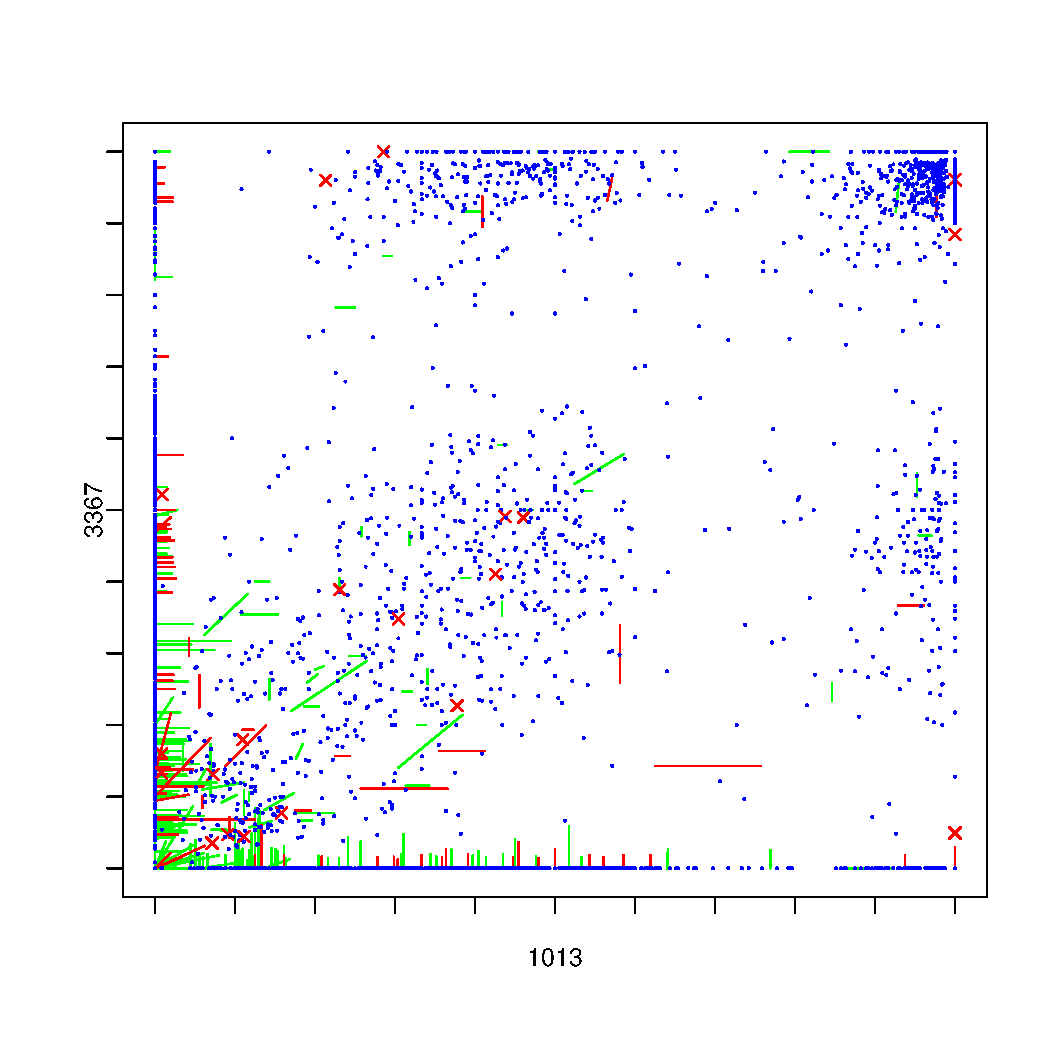
\includegraphics[width=7in]{Fig1-mscat-figs/unnamed-chunk-45-1} 

\end{knitrout}

Finally, what should we show in the main text figure?  Not this, it's too complicated.  Showing it either before filtering (the original plots) or after preserves the interesting 4-lobed structure, so that's not an issue.  The main issue is what is clearest/simplest to explain.  I currently favor julie.filter1=0 and julie.filter2=TRUE, but flag inconsistent points, say, in red.  Explanation is roughly we kept all data, but only used the most frequent nonref nucleotide, flagging cases where that is different between the two strains; it will be obvious by eye that most points are consistent, and the rare inconsistent ones cluster near the axes.

\subsection{Other measures of discordance}

I think the analysis in the previous subsection is the most straightforward way to address the question, but I tried some other stuff earlier that gives other ways of viewing it.  I will leave it here for posterity, but just skim it or skip it.

{\footnotesize
How many selected positions are called SNPs in at least one strain?

\begin{knitrout}\scriptsize
\definecolor{shadecolor}{rgb}{0.969, 0.969, 0.969}\color{fgcolor}\begin{kframe}
\begin{alltt}
\hlstd{the.snps} \hlkwb{<-} \hlstd{(snp.tables[[}\hlnum{1}\hlstd{]]}\hlopt{$}\hlstd{snp}\hlopt{==}\hlnum{1}\hlstd{)}
\hlkwa{for}\hlstd{(i} \hlkwa{in} \hlnum{2}\hlopt{:}\hlnum{7}\hlstd{)\{}
  \hlstd{the.snps} \hlkwb{<-} \hlstd{the.snps} \hlopt{|} \hlstd{(snp.tables[[i]]}\hlopt{$}\hlstd{snp}\hlopt{==}\hlnum{1}\hlstd{)}
\hlstd{\}}
\hlstd{n} \hlkwb{<-} \hlkwd{sum}\hlstd{(the.snps[selected])}
\hlkwd{cat}\hlstd{(n,} \hlstr{'of'}\hlstd{, n.selected,} \hlstr{'='}\hlstd{, n}\hlopt{/}\hlstd{n.selected}\hlopt{*}\hlnum{100}\hlstd{,} \hlstr{'%\textbackslash{}n'}\hlstd{)}
\end{alltt}
\begin{verbatim}
# 3820 of 5213 = 73.27834 %
\end{verbatim}
\end{kframe}
\end{knitrout}

Are they ``consistent SNPs,'' as in shared-SNPs analysis?

\textit{Uh oh.  As of 10/2015, ``../00common/mycache/consistent.rda'' no longer exists, so following code breaks.  I think this has been subsumed by one of the several files named:}
\begin{verbatim}
  paste('../00common/mycache/filtered.snps', which.snp.tables(), 'rda', sep='.')
\end{verbatim}
\noindent\textit{but not totally sure and I think the structure has changed, too.  E.g., I think the embedded var name ``consistent'' should now be} \verb|filtered.snps$Data$consistent.snps| \textit{or something.  Maybe I've fixed this below, maybe not; but not on the critical path tonight...}

\begin{knitrout}\scriptsize
\definecolor{shadecolor}{rgb}{0.969, 0.969, 0.969}\color{fgcolor}\begin{kframe}
\begin{alltt}
\hlcom{#old:}
\hlcom{#load('../00common/mycache/consistent.rda')}
\hlcom{#str(consistent)}
\hlcom{#sum(consistent[[2]])}
\hlcom{#conswhere <- names(consistent[[2]][consistent[[2]]])}
\hlcom{#new:}
\hlkwd{load}\hlstd{(}\hlstr{'../00common/mycache/filtered.snps.Chr1-qfiltered.rda'}\hlstd{)}
\hlkwd{str}\hlstd{(filtered.snps}\hlopt{$}\hlstd{Data}\hlopt{$}\hlstd{consistent.snps)}
\end{alltt}
\begin{verbatim}
# List of 4
#  $ : Named logi [1:47499] TRUE FALSE TRUE TRUE TRUE TRUE ...
#   ..- attr(*, "names")= chr [1:47499] "Chr1:333" "Chr1:417" "Chr1:435" "Chr1:438" ...
#  $ : Named logi [1:47499] TRUE TRUE TRUE TRUE TRUE TRUE ...
#   ..- attr(*, "names")= chr [1:47499] "Chr1:333" "Chr1:417" "Chr1:435" "Chr1:438" ...
#  $ : Named logi [1:47499] TRUE TRUE TRUE TRUE TRUE TRUE ...
#   ..- attr(*, "names")= chr [1:47499] "Chr1:333" "Chr1:417" "Chr1:435" "Chr1:438" ...
#  $ : Named logi [1:47499] TRUE TRUE TRUE TRUE TRUE TRUE ...
#   ..- attr(*, "names")= chr [1:47499] "Chr1:333" "Chr1:417" "Chr1:435" "Chr1:438" ...
\end{verbatim}
\begin{alltt}
\hlstd{consistent} \hlkwb{<-} \hlstd{filtered.snps}\hlopt{$}\hlstd{Data}\hlopt{$}\hlstd{consistent.snps}
\hlkwd{sum}\hlstd{(consistent[[}\hlnum{2}\hlstd{]])}
\end{alltt}
\begin{verbatim}
# [1] 47108
\end{verbatim}
\begin{alltt}
\hlstd{conswhere} \hlkwb{<-} \hlkwd{names}\hlstd{(consistent[[}\hlnum{2}\hlstd{]][consistent[[}\hlnum{2}\hlstd{]]])}

\hlstd{conswhere[}\hlnum{1}\hlopt{:}\hlnum{10}\hlstd{]}
\end{alltt}
\begin{verbatim}
#  [1] "Chr1:333" "Chr1:417" "Chr1:435" "Chr1:438" "Chr1:465" "Chr1:560" "Chr1:567" "Chr1:723"
#  [9] "Chr1:735" "Chr1:858"
\end{verbatim}
\begin{alltt}
\hlstd{conswherei} \hlkwb{<-} \hlkwd{as.integer}\hlstd{(}\hlkwd{substr}\hlstd{(conswhere,}\hlnum{6}\hlstd{,}\hlnum{99}\hlstd{))}
\hlkwd{str}\hlstd{(conswherei)}
\end{alltt}
\begin{verbatim}
#  int [1:47108] 333 417 435 438 465 560 567 723 735 858 ...
\end{verbatim}
\begin{alltt}
\hlkwd{seecounts}\hlstd{(conswherei[}\hlkwd{sample.int}\hlstd{(}\hlkwd{length}\hlstd{(conswherei),}\hlnum{10}\hlstd{)],}\hlkwc{snp.tables}\hlstd{=snp.tables)} \hlcom{# eyeball a few}
\end{alltt}
\begin{verbatim}
#     chr     pos Ref Strain   A   G  C  T SNP  exon indel nrf rat
# 1  Chr1  833617   C                                             
# 2                     1007   0   0 25  0   0 FALSE FALSE        
# 3                     1012   0   0 51  0   0 FALSE FALSE        
# 4                     1013   0   0 28 16   1 FALSE FALSE        
# 5                     1014   0   0 13  0   0 FALSE FALSE        
# 6                     1015   0   0 50  0   0 FALSE FALSE        
# 7                     3367   0   0 22 25   1 FALSE FALSE        
# 8                     1335   0   0 95  0   0 FALSE FALSE        
# 9  Chr1 1150017   A                                             
# 10                    1007  19   0  0  8   1  TRUE FALSE        
# 11                    1012  30   0  0 17   1  TRUE FALSE        
# 12                    1013  65   0  0  0   0  TRUE FALSE        
# 13                    1014  10   0  0  3   1  TRUE FALSE        
# 14                    1015  30   0  0 21   1  TRUE FALSE        
# 15                    3367  51   0  0  0   0  TRUE FALSE        
# 16                    1335  49   0  0 33   1  TRUE FALSE        
# 17 Chr1 1812033   A                                             
# 18                    1007  21  23  0  0   1  TRUE FALSE        
# 19                    1012  35  32  0  0   1  TRUE FALSE        
# 20                    1013  22  26  0  0   1  TRUE FALSE        
# 21                    1014  19   8  0  0   1  TRUE FALSE        
# 22                    1015  18  48  0  0   1  TRUE FALSE        
# 23                    3367  26   0  0  0   0  TRUE FALSE        
# 24                    1335  10   3  0  0   1  TRUE FALSE        
# 25 Chr1 2799854   A                                             
# 26                    1007   9   0  0  0   0 FALSE FALSE        
# 27                    1012  35   0  0  0   0 FALSE FALSE        
# 28                    1013  23   0 15  0   1 FALSE FALSE        
# 29                    1014   8   0  0  0   0 FALSE FALSE        
# 30                    1015  32   0  0  0   0 FALSE FALSE        
# 31                    3367   0   0 23  0   1 FALSE FALSE        
# 32                    1335 119   0  0  0   0 FALSE FALSE        
# 33 Chr1  631862   C                                             
# 34                    1007   0   0 13  0   0 FALSE FALSE        
# 35                    1012   0   0 20  0   0 FALSE FALSE        
# 36                    1013   0   0 12  0   0 FALSE FALSE        
# 37                    1014   0   0  6  0   0 FALSE FALSE        
# 38                    1015   0   0  5 10   1 FALSE FALSE        
# 39                    3367   0   0 24  0   0 FALSE FALSE        
# 40                    1335   0   0 27  0   0 FALSE FALSE        
# 41 Chr1 2774888   G                                             
# 42                    1007   0  21  0  0   0  TRUE FALSE        
# 43                    1012   0  44  0  0   0  TRUE FALSE        
# 44                    1013   0   4 13  0   1  TRUE FALSE        
# 45                    1014   0   7  0  0   0  TRUE FALSE        
# 46                    1015   0  53  0  0   0  TRUE FALSE        
# 47                    3367   0  44  0  0   0  TRUE FALSE        
# 48                    1335   0 111  0  0   0  TRUE FALSE        
# 49 Chr1 2902959   C                                             
# 50                    1007   0   0 34  0   0 FALSE FALSE        
# 51                    1012   0   0 73  0   0 FALSE FALSE        
# 52                    1013   0   0 51 22   1 FALSE FALSE        
# 53                    1014   0   0 24  0   0 FALSE FALSE        
# 54                    1015   0   0 63  0   0 FALSE FALSE        
# 55                    3367   0   0 34 19   1 FALSE FALSE        
# 56                    1335   0   0 90  0   0 FALSE FALSE        
# 57 Chr1 2067941   G                                             
# 58                    1007   0  21 10  0   1  TRUE FALSE        
# 59                    1012   0  15 23  0   1  TRUE FALSE        
# 60                    1013   0  32  0  0   0  TRUE FALSE        
# 61                    1014   0   4  1  0   0  TRUE FALSE        
# 62                    1015   0  21 21  0   1  TRUE FALSE        
# 63                    3367   0  40  0  0   0  TRUE FALSE        
# 64                    1335   0  31 34  0   1  TRUE FALSE        
# 65 Chr1 1970279   G                                             
# 66                    1007   0  15  0  2   0 FALSE FALSE        
# 67                    1012   0  12  0  5   1 FALSE FALSE        
# 68                    1013   0  16  1  1   0 FALSE FALSE        
# 69                    1014   0   3  0  0   0 FALSE FALSE        
# 70                    1015   0  18  0  3   0 FALSE FALSE        
# 71                    3367   0  13  0  0   0 FALSE FALSE        
# 72                    1335   0  16  0  2   0 FALSE FALSE        
# 73 Chr1  181945   C                                             
# 74                    1007   0   0 31  0   0 FALSE FALSE        
# 75                    1012   0   0 55  0   0 FALSE FALSE        
# 76                    1013  15   0 19  0   1 FALSE FALSE        
# 77                    1014   0   0 26  0   0 FALSE FALSE        
# 78                    1015   0   0 51  0   0 FALSE FALSE        
# 79                    3367   0   0 32  0   0 FALSE FALSE        
# 80                    1335   0   0 56  0   0 FALSE FALSE
\end{verbatim}
\begin{alltt}
\hlstd{longcons} \hlkwb{<-} \hlkwd{vector}\hlstd{(}\hlstr{'logical'}\hlstd{,}\hlkwd{length}\hlstd{(the.snps))}
\hlstd{longcons[conswherei]} \hlkwb{<-} \hlstd{T}
\hlkwd{cat}\hlstd{(}\hlstr{'selected:'}\hlstd{, n.selected,} \hlstr{'consistent:'}\hlstd{,}\hlkwd{length}\hlstd{(conswherei),} \hlstr{'both:'}\hlstd{,} \hlkwd{sum}\hlstd{(longcons} \hlopt{&} \hlstd{longsel),}
    \hlstr{'='}\hlstd{,} \hlkwd{sum}\hlstd{(longcons} \hlopt{&} \hlstd{longsel)}\hlopt{/}\hlstd{n.selected}\hlopt{*}\hlnum{100}\hlstd{,} \hlstr{'%\textbackslash{}n'}\hlstd{)}
\end{alltt}
\begin{verbatim}
# selected: 5213 consistent: 47108 both: 3794 = 72.77959 %
\end{verbatim}
\end{kframe}
\end{knitrout}

I.e., nearly all positions selected for the pairs plots that are called SNPs somewhere, are classified as ``consistent'' in the shared-SNPs analysis.

How many selected positions have 0,1,2,3 nonzero nonref counts, per strain:

\begin{knitrout}\scriptsize
\definecolor{shadecolor}{rgb}{0.969, 0.969, 0.969}\color{fgcolor}\begin{kframe}
\begin{alltt}
\hlstd{see.nrf.counts} \hlkwb{<-} \hlkwa{function}\hlstd{(}\hlkwc{sel}\hlstd{=selected,} \hlkwc{lo}\hlstd{=}\hlnum{0}\hlstd{,} \hlkwc{snp.tables}\hlstd{=snp.tables.01.26.14)\{}
  \hlstd{n.sel} \hlkwb{<-} \hlkwd{length}\hlstd{(sel)}
  \hlstd{counts} \hlkwb{<-} \hlkwa{NULL}
  \hlstd{aggreg8} \hlkwb{<-} \hlkwd{matrix}\hlstd{(}\hlnum{0}\hlstd{,n.sel,}\hlnum{6}\hlstd{)}
  \hlkwd{colnames}\hlstd{(aggreg8)} \hlkwb{<-} \hlkwd{c}\hlstd{(}\hlstr{'Cov'}\hlstd{,}\hlstr{'a'}\hlstd{,}\hlstr{'g'}\hlstd{,}\hlstr{'c'}\hlstd{,}\hlstr{'t'}\hlstd{,}\hlstr{'.match'}\hlstd{)}
  \hlkwa{for}\hlstd{(st} \hlkwa{in} \hlnum{1}\hlopt{:}\hlnum{7}\hlstd{)\{}
    \hlcom{# extract the selected subset of positions in one strain}
    \hlstd{sel.df} \hlkwb{<-} \hlstd{snp.tables[[st]][sel,]}
    \hlcom{# count nonzero nonref nucleotides (more generally, if lo > 0, count those > lo)}
    \hlstd{sel.nz} \hlkwb{<-} \hlstd{(sel.df}\hlopt{$}\hlstd{a} \hlopt{>} \hlstd{lo)} \hlopt{+} \hlstd{(sel.df}\hlopt{$}\hlstd{g} \hlopt{>} \hlstd{lo)} \hlopt{+} \hlstd{(sel.df}\hlopt{$}\hlstd{c} \hlopt{>} \hlstd{lo)} \hlopt{+} \hlstd{(sel.df}\hlopt{$}\hlstd{t} \hlopt{>} \hlstd{lo)}
    \hlcom{#print(summary(sel.nz))}
    \hlcom{# use "histogram" to count them}
    \hlstd{counts} \hlkwb{<-} \hlkwd{rbind}\hlstd{(counts,} \hlkwd{hist}\hlstd{(sel.nz,}\hlkwc{breaks}\hlstd{=}\hlopt{-}\hlnum{1}\hlopt{:}\hlnum{3}\hlstd{,}\hlkwc{plot}\hlstd{=F)}\hlopt{$}\hlstd{counts)}
    \hlcom{# also aggregate counts across all 7}
    \hlstd{aggreg8[,}\hlstr{'Cov'}\hlstd{]}    \hlkwb{<-} \hlstd{aggreg8[,}\hlstr{'Cov'}\hlstd{]}    \hlopt{+} \hlstd{sel.df[,}\hlstr{'Cov'}\hlstd{]}
    \hlstd{aggreg8[,}\hlstr{'.match'}\hlstd{]} \hlkwb{<-} \hlstd{aggreg8[,}\hlstr{'.match'}\hlstd{]} \hlopt{+} \hlstd{sel.df[,}\hlstr{'.match'}\hlstd{]}
    \hlkwa{for}\hlstd{(nuc} \hlkwa{in} \hlkwd{c}\hlstd{(}\hlstr{'a'}\hlstd{,}\hlstr{'g'}\hlstd{,}\hlstr{'c'}\hlstd{,}\hlstr{'t'}\hlstd{))\{}
      \hlstd{aggreg8[,nuc]} \hlkwb{<-} \hlstd{aggreg8[,nuc]} \hlopt{+} \hlkwd{ifelse}\hlstd{(sel.df[,nuc]} \hlopt{<=} \hlstd{lo,} \hlnum{0}\hlstd{, sel.df[,nuc])}
    \hlstd{\}}
  \hlstd{\}}
  \hlcom{# same counting for the aggregate (if >lo individually, then >lo in aggregate, so >0 test ok here)}
  \hlstd{agg.nz} \hlkwb{<-} \hlstd{(aggreg8[,}\hlstr{'a'}\hlstd{]} \hlopt{>} \hlnum{0}\hlstd{)} \hlopt{+} \hlstd{(aggreg8[,}\hlstr{'g'}\hlstd{]} \hlopt{>} \hlnum{0}\hlstd{)} \hlopt{+} \hlstd{(aggreg8[,}\hlstr{'c'}\hlstd{]} \hlopt{>} \hlnum{0}\hlstd{)} \hlopt{+} \hlstd{(aggreg8[,}\hlstr{'t'}\hlstd{]} \hlopt{>} \hlnum{0}\hlstd{)}
  \hlstd{counts} \hlkwb{<-} \hlkwd{rbind}\hlstd{(counts,} \hlkwd{hist}\hlstd{(agg.nz,}\hlkwc{breaks}\hlstd{=}\hlopt{-}\hlnum{1}\hlopt{:}\hlnum{3}\hlstd{,}\hlkwc{plot}\hlstd{=F)}\hlopt{$}\hlstd{counts)}
  \hlkwd{rownames}\hlstd{(counts)} \hlkwb{<-} \hlkwd{c}\hlstd{(}\hlkwd{names}\hlstd{(snp.tables),} \hlstr{'aggregate'}\hlstd{)}
  \hlkwd{colnames}\hlstd{(counts)} \hlkwb{<-} \hlkwd{c}\hlstd{(}\hlstr{'zero'}\hlstd{,} \hlstr{'one'}\hlstd{,} \hlstr{'two'}\hlstd{,} \hlstr{'three'}\hlstd{)}
  \hlkwd{return}\hlstd{(counts)}
\hlstd{\}}
\hlkwd{see.nrf.counts}\hlstd{(}\hlkwc{lo}\hlstd{=}\hlnum{0}\hlstd{,} \hlkwc{snp.tables}\hlstd{=snp.tables)}
\end{alltt}
\begin{verbatim}
#           zero  one two three
# 1007      3433 1740  40     0
# 1012      3373 1799  40     1
# 1013      1908 3179 123     3
# 1014      3362 1771  73     7
# 1015      3357 1807  49     0
# 3367      1949 3163 101     0
# 1335      3391 1764  57     1
# aggregate    0 4525 655    33
\end{verbatim}
\end{kframe}
\end{knitrout}


In short, of the 5213 selected positions, in all strains, very roughly half of these positions have \emph{no} nonreference reads, most of the rest have nonreference reads for a single nucleotide, 2--10\% percent have nonzero read counts for two different nonref nucleotides and a fraction of a per cent show reads for all three.  These numbers shift sharply when aggregating read counts across all 7 strains.  \emph{However}, many of these totals seem to be largely driven by very low read counts; deleting singletons (1 read in a given nonref nuc in any strain) reduces the 3616 positions having three nonref nucleotides to a mere 87, and deleting doubletons further reduces it to 18:

\begin{knitrout}\scriptsize
\definecolor{shadecolor}{rgb}{0.969, 0.969, 0.969}\color{fgcolor}\begin{kframe}
\begin{alltt}
\hlkwd{see.nrf.counts}\hlstd{(}\hlkwc{lo}\hlstd{=}\hlnum{1}\hlstd{,} \hlkwc{snp.tables}\hlstd{=snp.tables)}
\end{alltt}
\begin{verbatim}
#           zero  one two three
# 1007      3578 1629   6     0
# 1012      3511 1692  10     0
# 1013      2055 3123  33     2
# 1014      3575 1614  23     1
# 1015      3489 1711  13     0
# 3367      2050 3133  30     0
# 1335      3558 1639  16     0
# aggregate    2 5062 142     7
\end{verbatim}
\begin{alltt}
\hlkwd{see.nrf.counts}\hlstd{(}\hlkwc{lo}\hlstd{=}\hlnum{2}\hlstd{,} \hlkwc{snp.tables}\hlstd{=snp.tables)}
\end{alltt}
\begin{verbatim}
#           zero  one two three
# 1007      3675 1535   3     0
# 1012      3574 1633   6     0
# 1013      2111 3075  26     1
# 1014      3744 1462   6     1
# 1015      3550 1659   4     0
# 3367      2089 3102  22     0
# 1335      3623 1580  10     0
# aggregate   22 5088 100     3
\end{verbatim}
\end{kframe}
\end{knitrout}

}%end \footnotesize

\subsection{Discordance in UN-selected positions}

Out of curiousity, how many positions in Italy have all nonzero counts on all three nonref nucs, across all of Chr1, not just the set selected for the pairwise comparisons?

\begin{knitrout}\footnotesize
\definecolor{shadecolor}{rgb}{0.969, 0.969, 0.969}\color{fgcolor}\begin{kframe}
\begin{alltt}
\hlcom{# look for 3 nonref cases, all of Chr1}
\hlstd{italy.nz} \hlkwb{<-} \hlstd{(snp.tables[[}\hlnum{6}\hlstd{]]}\hlopt{$}\hlstd{a} \hlopt{>} \hlnum{0}\hlstd{)} \hlopt{+} \hlstd{(snp.tables[[}\hlnum{6}\hlstd{]]}\hlopt{$}\hlstd{g} \hlopt{>} \hlnum{0}\hlstd{)} \hlopt{+}
            \hlstd{(snp.tables[[}\hlnum{6}\hlstd{]]}\hlopt{$}\hlstd{c} \hlopt{>} \hlnum{0}\hlstd{)} \hlopt{+} \hlstd{(snp.tables[[}\hlnum{6}\hlstd{]]}\hlopt{$}\hlstd{t} \hlopt{>} \hlnum{0}\hlstd{)}
\hlstd{italy.3}  \hlkwb{<-} \hlkwd{sum}\hlstd{(italy.nz} \hlopt{==} \hlnum{3}\hlstd{)}
\hlstd{italy.which3} \hlkwb{<-} \hlkwd{which}\hlstd{(italy.nz} \hlopt{==} \hlnum{3}\hlstd{)}
\hlkwd{cat}\hlstd{(}\hlstr{'Italy has'}\hlstd{, italy.3,} \hlstr{'positions with nonzero read counts for all 3 nonref nucs.\textbackslash{}n'}\hlstd{)}
\end{alltt}
\begin{verbatim}
# Italy has 17 positions with nonzero read counts for all 3 nonref nucs.
\end{verbatim}
\begin{alltt}
\hlcom{# coverage summary}
\hlkwd{summary}\hlstd{(snp.tables[[}\hlnum{6}\hlstd{]]}\hlopt{$}\hlstd{Cov[italy.nz} \hlopt{==} \hlnum{3}\hlstd{])}
\end{alltt}
\begin{verbatim}
#    Min. 1st Qu.  Median    Mean 3rd Qu.    Max. 
#     5.0    23.0    76.0   103.8   139.0   363.0
\end{verbatim}
\begin{alltt}
\hlcom{# nonref count summary}
\hlkwd{summary}\hlstd{(snp.tables[[}\hlnum{6}\hlstd{]]}\hlopt{$}\hlstd{Cov[italy.nz} \hlopt{==} \hlnum{3}\hlstd{]} \hlopt{-} \hlstd{snp.tables[[}\hlnum{6}\hlstd{]]}\hlopt{$}\hlstd{.match[italy.nz} \hlopt{==} \hlnum{3}\hlstd{])}
\end{alltt}
\begin{verbatim}
#    Min. 1st Qu.  Median    Mean 3rd Qu.    Max. 
#    3.00    5.00   11.00   19.41   22.00   99.00
\end{verbatim}
\begin{alltt}
\hlcom{# first few examples}
\hlstd{snp.tables[[}\hlnum{6}\hlstd{]][italy.which3[}\hlnum{1}\hlopt{:}\hlnum{9}\hlstd{],]}
\end{alltt}
\begin{verbatim}
#         snp  Chr     Pos Ref Cov  a g  c  t n .match  exon indel  chr     pos rawCov
# 258626    1 Chr1  258626   T  28  1 1 13  0 0     13  TRUE FALSE Chr1  258626     51
# 346940    0 Chr1  346940   C 175  1 1  0  1 0    172 FALSE FALSE Chr1  346940    229
# 700466    0 Chr1  700466   G  33 10 0  1  1 0     21 FALSE FALSE Chr1  700466     47
# 718157    0 Chr1  718157   G  23  2 0  1  1 0     19  TRUE FALSE Chr1  718157     35
# 1116985   0 Chr1 1116985   C 133 24 5  0  5 0     99  TRUE FALSE Chr1 1116985    187
# 1117075   1 Chr1 1117075   G 363 72 0 14 13 0    264  TRUE FALSE Chr1 1117075    421
# 1117218   0 Chr1 1117218   A  99  0 1  2  8 0     88  TRUE FALSE Chr1 1117218    140
# 1117276   0 Chr1 1117276   G  76  8 0  1  2 0     65  TRUE FALSE Chr1 1117276     87
# 1224654   0 Chr1 1224654   T   8  2 3  1  0 0      2  TRUE FALSE Chr1 1224654     18
\end{verbatim}
\end{kframe}
\end{knitrout}

Answer: 17.  Their overall coverage is unremarkable (except perhaps the extreme outliers), but the fact that the total nonref count is $\leq 7$ in three quarters of the cases (implying a max count of no more than 5 in these cases) and the mean is $<9$ suggests that these are dominated by low-count sporadic read errors rather than biology.  However, the second example above (Chr1  9310) looks like a plausible tri-allelic (but not quad-) position.

\textbf{Section \ref{sec:post} Summary:} Based on the criteria outlined in subsection \ref{sec:filtering}, the nonreference frequencies at positions selected for display in the pairwise scatter plots definitely include counts for discordant nucleotides, e.g., a read for a nonreference ``A'' at some position in one strain where a read for a ``G'' is seen in a different strain.  But in the vast majority of cases,  discordant counts are small, and the big picture does not change if we do some further filtering to remove them.

\section{Tangents}
1: I wondered what the analogous plots would look like for the big desert region.  Answer is more or less as expected: based on these 5686  points, the 5 NE have a thin, somewhat correlated, scatter of points above freq .2, and a cloud below .2.  There is no clear signal to suggest whether this cloud is low-freq alleles vs  read errors.  In this region, Italy and Wales have many apparent SNPs absent from the 5 NE, showing a pattern of sharing similar to the (largely) nondesert in the main fig 1b above.

\begin{knitrout}\footnotesize
\definecolor{shadecolor}{rgb}{0.969, 0.969, 0.969}\color{fgcolor}\begin{kframe}
\begin{alltt}
\hlstd{pi} \hlkwb{<-} \hlkwd{order}\hlstd{(des[[}\hlnum{1}\hlstd{]][[}\hlnum{1}\hlstd{]][,}\hlnum{3}\hlstd{],}\hlkwc{decreasing}\hlstd{=T)}
\hlstd{big} \hlkwb{<-} \hlstd{pi[}\hlnum{1}\hlstd{]}

\hlkwd{nrf.6plus1}\hlstd{(}\hlkwc{snp.tables}\hlstd{=snp.tables,}
           \hlkwc{mask}\hlstd{=}\hlkwd{seg.mask}\hlstd{(des[[}\hlnum{1}\hlstd{]][[}\hlnum{1}\hlstd{]][big,}\hlnum{1}\hlstd{],des[[}\hlnum{1}\hlstd{]][[}\hlnum{1}\hlstd{]][big,}\hlnum{2}\hlstd{],}
                         \hlkwc{snp.tables}\hlstd{=snp.tables))}
\end{alltt}
\begin{verbatim}
# non-null mask 320006 positions.
# nrf.6plus1: From a region of length: 320006 we identified all positions satisfying: 
#  21 <= coverage <= 150 in *all* 7 isolates, 
# and having 0.1 <= nr.frac <= 1.0 in *at least 1* of them. 
# From these 409 positions, we sampled 10000 to plot.
\end{verbatim}
\end{kframe}\begin{figure}
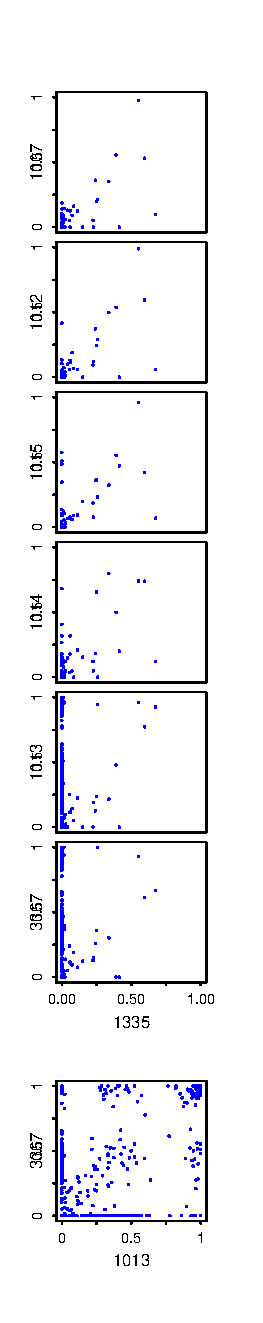
\includegraphics[width=\maxwidth]{Fig1-mscat-figs/6plus1-for-big-desert-1} \caption[Comparative nonref allele proportions in Chr1 big desert]{Comparative nonref allele proportions in Chr1 big desert.}\label{fig:6plus1-for-big-desert}
\end{figure}


\end{knitrout}

\section{To Do/Improvements?}

\iffalse
I think the axis labels take up more space than is reasonable, would look better if a bit more compact.  The best resource I've seen on this is:
\href{http://www.carlislerainey.com/2012/12/17/controlling-axes-of-r-plots/}{http://www.carlislerainey.com/2012/12/17/controlling-axes-of-r-plots/}

NOTE: as of 8/8/18 (well, it said ``18'', but as of 10/2015, I think that probably was '14), this has been done, based on Rainey's \texttt{compactr} package.
\fi

On 2015/11/7 \& 8 I did a bit more exporlatory stuff to see whether we could clarify the Gyre data.  My conclusion is --- not without a lot of work.  It looks better in the un-q-filtered data, but of course then IT/Wales have peak at 0.8 rather than 1.  With current q-filtering, the later problem is fixed, but mean coverage in Gyre drops sharply, to about 12:

\begin{knitrout}\footnotesize
\definecolor{shadecolor}{rgb}{0.969, 0.969, 0.969}\color{fgcolor}\begin{kframe}
\begin{alltt}
\hlkwd{summary}\hlstd{(snp.tables[[}\hlnum{4}\hlstd{]]}\hlopt{$}\hlstd{Cov)} \hlcom{# weak coverage in Gyre}
\end{alltt}
\begin{verbatim}
#    Min. 1st Qu.  Median    Mean 3rd Qu.    Max. 
#    0.00    7.00   11.00   12.43   16.00  212.00
\end{verbatim}
\begin{alltt}
\hlkwd{unlist}\hlstd{(}\hlkwd{lapply}\hlstd{(snp.tables,} \hlkwa{function}\hlstd{(}\hlkwc{x}\hlstd{)\{}\hlkwd{median}\hlstd{(x}\hlopt{$}\hlstd{Cov)\}))}
\end{alltt}
\begin{verbatim}
# 1007 1012 1013 1014 1015 3367 1335 
#   27   47   40   11   45   43   79
\end{verbatim}
\end{kframe}
\end{knitrout}

With the current filtering, based on min/max count limits applied uniformly across all strains, presently [10, 120] for the scatter-smooths plots, the ``10'' end means that we loose a lot of Gyre while scooping up noise in the others, while the 120 end gets collapsed repeats etc in gyre.  I tried lowering the 10 to 9, 7, even 5 (thinking this might get more good data in Gyre), and tried raising it 15 or 20 (thinking it would get less data, but perhap the het positions would stand out better).  But it didn't help; all figures looked pretty much the same.  Setting julie.filter1=2 \emph{did} remove big spikes near zero (plausibly 1 or 2 isolated read errors at many positions, still not removed by q-filters), and created a very broad hump (roughly 0.2-0.8), but this seems a bit arbitrary; not fruitful to show it in the paper.   With the 7x difference in median coverage across strains, I think a better way to choose the positions included in the scatters would be to find the set of positions that are, say, $\mu\pm\sigma$ simultaneously in all 7, using per-strain values for $\mu,\sigma$.   I don't expect the plots would change qualitatively, but I think this would cover more positions without pulling in unusually noisy ones, maybe giving a somewhat cleaner picture.  I have \emph{not} tried this yet.

I also ran it once on full genome data.  As expected, count of eligible position increased by about 10x, and histos are a bit smoother, but otherwise not an increment worth the effort.  E.g., there are more outlier dots which just add clutter.


% remember to do this to enable Id keyword substution: svn propset svn:keywords Id fig1b.rnw 
\vfill\footnotesize\flushright SVN ID I miss you $ $Id: Fig1-mscat.rnw 2017-07-21 or later ruzzo $ $
\end{document}
